% Basic Knowledge: Cardano track study guide for team "Los Curiosos" (Shelfie)
% Build: latexmk -pdf main.tex
\documentclass[11pt,a4paper,oneside]{report}
\usepackage[T1]{fontenc}
\usepackage[utf8]{inputenc}
\usepackage{charter}
\usepackage[scale=0.92]{tgheros}
\usepackage{microtype}
\usepackage[margin=2.3cm,headheight=14pt]{geometry}
\usepackage[dvipsnames,svgnames,table]{xcolor}
\usepackage{tikz}
\usetikzlibrary{arrows.meta,positioning,shapes.geometric,shapes.misc,shapes.symbols,calc,fit,backgrounds,decorations.pathreplacing,shadows,matrix,chains}
\usepackage[most]{tcolorbox}
\usepackage{booktabs,tabularx,array,longtable,multirow}
\usepackage{enumitem}
\usepackage{pifont}
\usepackage{amsmath,amssymb}
\usepackage{listings}
\usepackage{titlesec}
\usepackage{fancyhdr}
\usepackage{parskip}
\usepackage[hidelinks]{hyperref}
\hypersetup{colorlinks=true,linkcolor=cBlue,urlcolor=cBlue}

% ---------- Palette ----------
\definecolor{cBlue}{HTML}{0033AD}     % Cardano blue
\definecolor{cSky}{HTML}{3D7BFF}
\definecolor{cTeal}{HTML}{0F9D8A}
\definecolor{cGreen}{HTML}{2E8B3A}
\definecolor{cOrange}{HTML}{E8770E}
\definecolor{cRed}{HTML}{C62828}
\definecolor{cPurple}{HTML}{6A3FB5}
\definecolor{cGold}{HTML}{C99A06}
\definecolor{cGrey}{HTML}{5F6670}
\definecolor{cLight}{HTML}{F3F6FB}

% ---------- Headings ----------
\titleformat{\chapter}[display]
  {\sffamily\bfseries\color{cBlue}}
  {\Large\MakeUppercase{\chaptertitlename}~\thechapter}
  {4pt}{\Huge}[{\color{cSky}\titlerule[1.2pt]}]
\titlespacing*{\chapter}{0pt}{0pt}{18pt}
\titleformat{\section}{\sffamily\Large\bfseries\color{cBlue}}{\thesection}{0.6em}{}
\titleformat{\subsection}{\sffamily\large\bfseries\color{cSky!80!black}}{\thesubsection}{0.6em}{}
\titleformat{\subsubsection}{\sffamily\normalsize\bfseries\color{cGrey}}{}{0em}{}
\setcounter{secnumdepth}{2}
\setcounter{tocdepth}{1}

\pagestyle{fancy}
\fancyhf{}
\fancyhead[L]{\sffamily\small\color{cGrey}Cardano Track · Basic Knowledge}
\fancyhead[R]{\sffamily\small\color{cGrey}\leftmark}
\fancyfoot[C]{\sffamily\small\thepage}
\renewcommand{\headrulewidth}{0.4pt}
\fancypagestyle{plain}{\fancyhf{}\fancyfoot[C]{\sffamily\small\thepage}\renewcommand{\headrulewidth}{0pt}}

\setlist{itemsep=2pt,topsep=4pt}
\setlength{\parskip}{5pt}

% ---------- Boxes ----------
% Usage: \begin{conceptbox}{Title} ... \end{conceptbox}
\newtcolorbox{conceptbox}[1]{enhanced,breakable,colback=cBlue!5,colframe=cBlue,
  fonttitle=\sffamily\bfseries,title={\ding{228}\ #1},arc=2mm,boxrule=0.8pt,left=6pt,right=6pt}
\newtcolorbox{examplebox}[1]{enhanced,breakable,colback=cGreen!5,colframe=cGreen,
  fonttitle=\sffamily\bfseries,title={Example: #1},arc=2mm,boxrule=0.8pt}
\newtcolorbox{analogybox}[1]{enhanced,breakable,colback=cOrange!6,colframe=cOrange,
  fonttitle=\sffamily\bfseries,title={Everyday analogy: #1},arc=2mm,boxrule=0.8pt}
\newtcolorbox{warningbox}[1]{enhanced,breakable,colback=cRed!5,colframe=cRed,
  fonttitle=\sffamily\bfseries,title={\ding{55}\ Common pitfall: #1},arc=2mm,boxrule=0.8pt}
\newtcolorbox{shelfiebox}[1]{enhanced,breakable,colback=cPurple!5,colframe=cPurple,
  fonttitle=\sffamily\bfseries,title={In Shelfie: #1},arc=2mm,boxrule=0.8pt}
\newtcolorbox{keypoints}{enhanced,breakable,colback=cGold!8,colframe=cGold,
  fonttitle=\sffamily\bfseries,title={\ding{72}\ Key takeaways},arc=2mm,boxrule=0.8pt}
\newtcolorbox{quizbox}{enhanced,breakable,colback=cTeal!5,colframe=cTeal,
  fonttitle=\sffamily\bfseries,title={? Check yourself},arc=2mm,boxrule=0.8pt}
% Inline term highlight for first definitions
\newcommand{\term}[1]{\textbf{\color{cBlue}#1}}
\newcommand{\code}[1]{\texttt{\small #1}}
\newcommand{\yes}{\textcolor{cGreen}{\ding{51}}}
\newcommand{\no}{\textcolor{cRed}{\ding{55}}}

% ---------- TikZ styles (shared by all chapters) ----------
\tikzset{
  >=Stealth,
  box/.style={draw,rounded corners=3pt,thick,align=center,font=\sffamily\small,minimum height=9mm,inner sep=5pt},
  actor/.style={box,fill=cBlue!10,draw=cBlue},
  agent/.style={box,fill=cPurple!12,draw=cPurple},
  human/.style={box,fill=cOrange!12,draw=cOrange},
  chain/.style={box,fill=cTeal!12,draw=cTeal},
  service/.style={box,fill=cGrey!10,draw=cGrey},
  good/.style={box,fill=cGreen!12,draw=cGreen},
  bad/.style={box,fill=cRed!10,draw=cRed},
  flow/.style={->,thick,draw=cGrey},
  pay/.style={->,very thick,draw=cGold!90!black},
  data/.style={->,thick,dashed,draw=cSky},
  lbl/.style={font=\sffamily\scriptsize,midway,fill=white,inner sep=1.5pt},
  blk/.style={draw=cBlue,fill=cBlue!8,thick,minimum width=2.4cm,minimum height=1.6cm,align=center,font=\sffamily\scriptsize},
  utxo/.style={draw=cTeal,fill=cTeal!15,thick,rounded corners=6pt,align=center,font=\sffamily\scriptsize,minimum width=2cm,minimum height=1cm},
}

\lstset{basicstyle=\ttfamily\small,backgroundcolor=\color{cLight},frame=single,rulecolor=\color{cGrey!40},
  breaklines=true,columns=fullflexible,keywordstyle=\color{cBlue}\bfseries,commentstyle=\color{cGrey}\itshape,
  stringstyle=\color{cGreen!70!black}}

\begin{document}

% ---------- Title page ----------
\begin{titlepage}
\begin{tikzpicture}[remember picture,overlay]
  \fill[cBlue] (current page.north west) rectangle ([yshift=-9cm]current page.north east);
  \foreach \i in {0,...,11}{
    \pgfmathsetmacro{\a}{\i*30}
    \fill[white,opacity=0.25] ([xshift=-3.2cm,yshift=-4.5cm]current page.north east) ++(\a:2.2cm) circle (2.5mm);
    \fill[white,opacity=0.45] ([xshift=-3.2cm,yshift=-4.5cm]current page.north east) ++(\a+15:1.3cm) circle (1.6mm);
  }
  \fill[white] ([xshift=-3.2cm,yshift=-4.5cm]current page.north east) circle (5mm);
  \node[anchor=north west,text=white,font=\sffamily\bfseries\fontsize{30}{36}\selectfont,align=left]
    at ([xshift=2.2cm,yshift=-2.6cm]current page.north west) {Basic Knowledge};
  \node[anchor=north west,text=white!85!cSky,font=\sffamily\Large,align=left]
    at ([xshift=2.2cm,yshift=-4.4cm]current page.north west)
    {Everything you need to understand\\the Cardano track and Shelfie};
\end{tikzpicture}
\vspace*{9.5cm}

{\sffamily\large
\textbf{TUM Blockchain \& AI Hackathon 2026}\\[2pt]
Track: \textcolor{cBlue}{\textbf{Agentic Commerce on Cardano}}\\[2pt]
Team \textit{Los Curiosos}: Helmut · Isabel · Fernando · Lorenz\par}
\vspace{1cm}

\begin{tcolorbox}[colback=cLight,colframe=cGrey!40,boxrule=0.5pt,arc=2mm]
\sffamily\small
\textbf{How to read this guide.} Part~I explains blockchains and Cardano from zero.
Part~II explains the payment and agent technologies of the track: HTTP~402, x402, AI agents,
Masumi and Sokosumi, and what ``on-chain'' really means. Part~III explains our own idea, Shelfie, and
how all the pieces fit together on hackathon day. Colour code of the boxes:\\[4pt]
\textcolor{cBlue}{\ding{110}} concept \quad
\textcolor{cGreen}{\ding{110}} example \quad
\textcolor{cOrange}{\ding{110}} everyday analogy \quad
\textcolor{cRed}{\ding{110}} pitfall \quad
\textcolor{cPurple}{\ding{110}} how Shelfie uses it \quad
\textcolor{cGold}{\ding{110}} takeaways \quad
\textcolor{cTeal}{\ding{110}} self-check
\end{tcolorbox}
\vfill
{\sffamily\small\color{cGrey} Study material, prepared before the build window. Facts about tools were taken from the
team's research notes (\texttt{investigacion/}, \texttt{diseno/}); anything marked \emph{verify Friday} is still unconfirmed.\par}
\end{titlepage}

\tableofcontents

\part{Foundations}
\chapter{Blockchain from zero}

\section*{Why this matters for us}
Shelfie pays real people (``workers'') for photographing price tags, and the AI agents in our system pay each other for services. All of these payments happen on a blockchain. You do not need to be a cryptography expert to build Shelfie, but you must understand what a blockchain \emph{is}, what a \emph{transaction} is, why a payment is ``final'', and why nobody can secretly change a receipt. This chapter explains the ideas one by one, with no prior knowledge assumed. Chapter~2 then narrows everything down to Cardano.

\section{What is a ledger, and why share it?}

A \term{ledger} is simply a list of records that says who owns what. A bank's database is a ledger: ``Anna has 120~EUR, Ben has 40~EUR.'' Every payment adds a line, for example ``Anna pays Ben 20~EUR''.

Normally one organisation owns the ledger (the bank). You must \emph{trust} that organisation: that it does not lose your line, does not change it, and does not refuse to show it to you.

A \term{distributed ledger} is a ledger that many independent computers keep \emph{at the same time}, each with its own full copy. A \term{blockchain} is the most common kind of distributed ledger. The computers follow shared rules to agree on which new lines are valid, so no single owner is needed.

\begin{figure}[h]
\centering
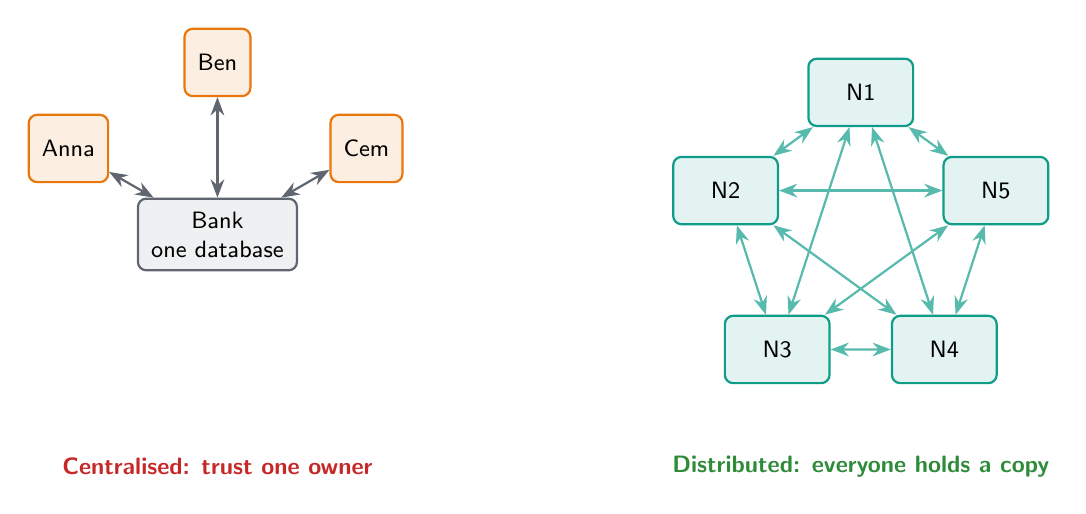
\begin{tikzpicture}[scale=0.95, transform shape]
  % left: central ledger
  \node[service] (bank) at (0,0) {Bank\\one database};
  \foreach \a/\n in {150/Anna,90/Ben,30/Cem}{
    \node[human] (u\n) at (\a:2.3cm) {\n};
    \draw[flow,<->] (u\n) -- (bank);
  }
  \node[font=\sffamily\bfseries\small,cRed] at (0,-3.1) {Centralised: trust one owner};
  % right: distributed
  \begin{scope}[xshift=8.6cm]
    \foreach \a/\n in {90/N1,162/N2,234/N3,306/N4,18/N5}{
      \node[chain,minimum width=1.4cm] (n\n) at (\a:1.9cm) {\n};
    }
    \foreach \x/\y in {N1/N2,N2/N3,N3/N4,N4/N5,N5/N1,N1/N3,N2/N4,N3/N5,N4/N1,N5/N2}{
      \draw[flow,<->,draw=cTeal!70] (n\x) -- (n\y);
    }
    \node[font=\sffamily\bfseries\small,cGreen] at (0,-3.1) {Distributed: everyone holds a copy};
  \end{scope}
\end{tikzpicture}
\caption{Left: a bank owns the only ledger. Right: many computers (nodes) each keep a full copy of the same ledger.}
\end{figure}

\begin{analogybox}{The village notebook}
Imagine a village where every sale is announced in the market square and \emph{every} villager writes it into their own notebook. If one villager tries to cheat by writing a different amount, the other 99 notebooks disagree with him and he is ignored. The ledger is ``true'' because the majority holds the same story, not because a boss says so.
\end{analogybox}

\subsection{What a shared ledger gives us}
\begin{itemize}
  \item \textbf{Transparency:} anyone can read the ledger (on public blockchains).
  \item \textbf{Tamper resistance:} changing history would require changing most copies at once.
  \item \textbf{No gatekeeper:} nobody can block you from sending a valid transaction.
  \item \textbf{Shared truth between strangers:} two parties who do not trust each other can still agree on ``this payment happened''.
\end{itemize}

\section{Hashes: digital fingerprints}

The most important tool in a blockchain is the \term{hash function}. It takes any data (a word, a photo, a whole book) and produces a fixed-length ``fingerprint'' called a \term{hash} or \term{digest}. The popular function SHA-256 always produces 256 bits, usually written as 64 hexadecimal characters.

A hash function has four properties that matter to us:
\begin{enumerate}
  \item \textbf{Deterministic:} the same input always gives the same hash.
  \item \textbf{Fixed size:} a 3-byte input and a 3-gigabyte input both give 64 hex characters.
  \item \textbf{One-way:} given a hash, you cannot work backwards to find the input.
  \item \textbf{Avalanche effect:} changing even one character of the input changes the hash completely and unpredictably.
\end{enumerate}

\begin{examplebox}{A tiny change, a totally different hash}
Real SHA-256 values (computed with the standard \code{sha256sum} tool):

\medskip
\begin{tabular}{@{}ll@{}}
\textbf{Input} & \textbf{SHA-256 (64 hex characters)}\\
\midrule
\texttt{Alice pays Bob 10} & \texttt{\scriptsize 69ad18dfd1ac4b3d711b02ee62caa00a82f0f67cc11ebacdd0c0ede0d8b6eaed}\\[3pt]
\texttt{Alice pays Bob 11} & \texttt{\scriptsize 83e970b5a467ce2dea0a573ee54380252a1d193b2625e2c29ad43ad6600990aa}\\[3pt]
\texttt{alice pays bob 10} & \texttt{\scriptsize be26845c48086d4f8edae714f8e48e32d806b4bcd4c054a0c19eb634b1f292a6}\\
\end{tabular}

\medskip
We changed one digit (10 to 11) or only the capital letters, and the result shares nothing recognisable with the original. If someone alters an old payment from 10 to 11, its hash no longer matches the one everybody stored, so the fraud is visible immediately.
\end{examplebox}

\begin{figure}[h]
\centering
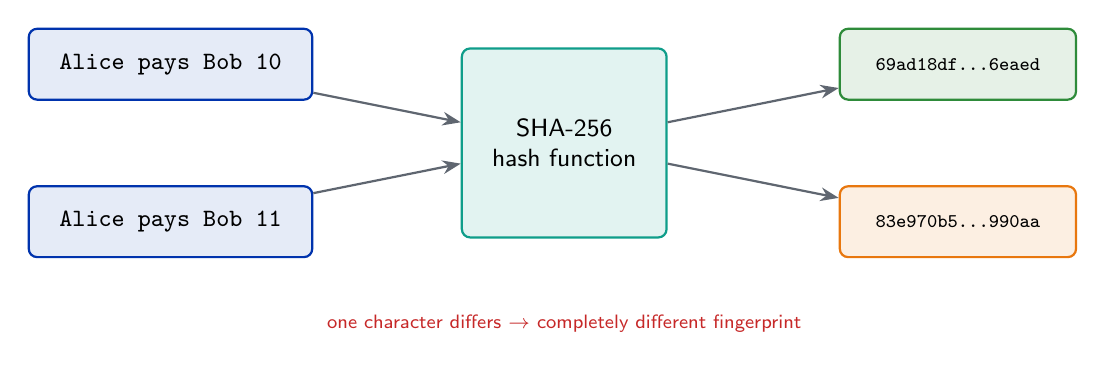
\begin{tikzpicture}
  \node[actor,minimum width=3.6cm] (in1) at (0,1.0) {\ttfamily\small Alice pays Bob 10};
  \node[actor,minimum width=3.6cm] (in2) at (0,-1.0) {\ttfamily\small Alice pays Bob 11};
  \node[chain,minimum width=2.6cm,minimum height=2.4cm] (h) at (5,0) {SHA-256\\hash function};
  \node[good,minimum width=3cm] (o1) at (10,1.0) {\ttfamily\scriptsize 69ad18df\ldots 6eaed};
  \node[good,minimum width=3cm,fill=cOrange!12,draw=cOrange] (o2) at (10,-1.0) {\ttfamily\scriptsize 83e970b5\ldots 990aa};
  \draw[flow] (in1) -- (h);
  \draw[flow] (in2) -- (h);
  \draw[flow] (h) -- (o1);
  \draw[flow] (h) -- (o2);
  \node[font=\sffamily\scriptsize,cRed] at (5,-2.3) {one character differs $\rightarrow$ completely different fingerprint};
\end{tikzpicture}
\caption{A hash function turns any input into a fixed-size fingerprint. Tiny input change, huge output change.}
\end{figure}

\begin{analogybox}{The tamper seal}
A hash works like a tamper-evident seal on a jar: you cannot tell what is inside from the seal, but if anybody opens the jar and closes it again, the seal no longer matches.
\end{analogybox}

\begin{shelfiebox}{Hashes appear everywhere}
Every Cardano transaction is identified by a hash (its \emph{tx hash}), which we will paste into an explorer as proof of payment. Shelfie also uses hash-like identifiers (idempotency keys, hashes of photos) to make sure a photo is paid for only once. See the verifier chapters later.
\end{shelfiebox}

\section{Keys and digital signatures}

\subsection{Public and private keys}
Hashes alone cannot prove \emph{who} authorised a payment. For that we use \term{public-key cryptography}. You create a pair of mathematically linked numbers:

\begin{itemize}
  \item the \term{private key} (also called secret key or signing key): kept secret; it is your power to authorise;
  \item the \term{public key}: can be shared with everybody; it lets others \emph{check} what the private key did.
\end{itemize}

You can derive the public key from the private key, but not the other way round (similar to the one-way property of hashes).

\begin{analogybox}{Mailbox and master key}
Your public key is like your mailbox address: everyone may know it and drop mail in. Your private key is the only key that opens the box and, in our case, also the only pen that can create your signature.
\end{analogybox}

\subsection{Digital signatures}
A \term{digital signature} is a short piece of data created from (a) a message and (b) your private key. Anybody who has your public key can verify that the signature is genuine and that the message was not changed afterwards. The private key is never revealed.

\begin{figure}[h]
\centering
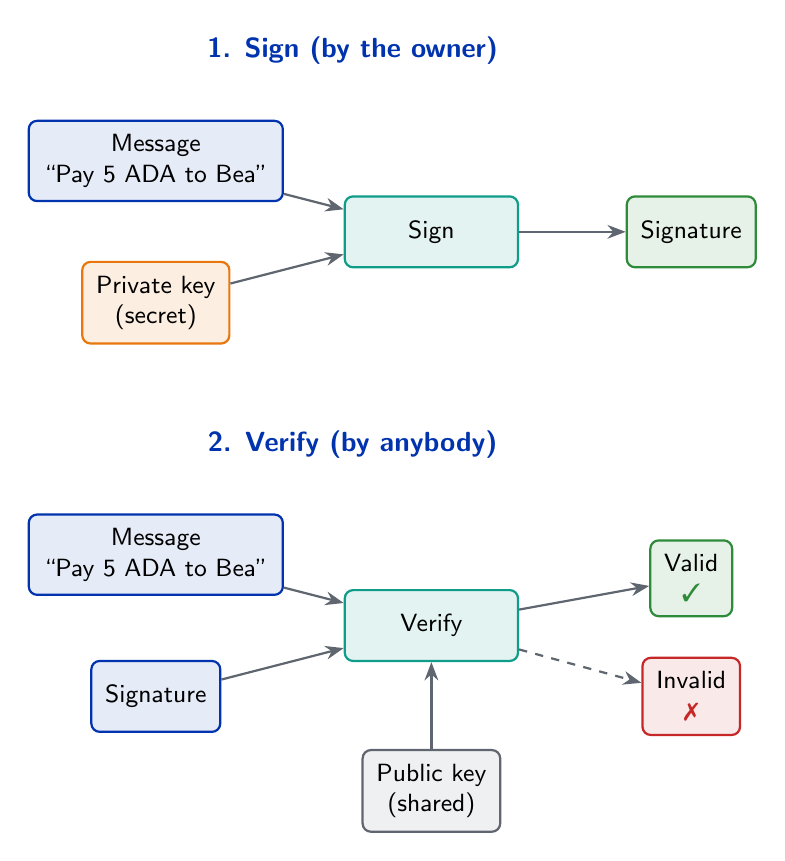
\begin{tikzpicture}[node distance=1.2cm]
  % SIGN
  \node[font=\sffamily\bfseries,cBlue] at (2.5,2.6) {1. Sign (by the owner)};
  \node[actor] (msg) at (0,1.2) {Message\\``Pay 5 ADA to Bea''};
  \node[human] (priv) at (0,-0.6) {Private key\\(secret)};
  \node[chain,minimum width=2.2cm] (sig) at (3.5,0.3) {Sign};
  \node[good] (s) at (6.8,0.3) {Signature};
  \draw[flow] (msg) -- (sig);
  \draw[flow] (priv) -- (sig);
  \draw[flow] (sig) -- (s);
  % VERIFY
  \begin{scope}[yshift=-5cm]
  \node[font=\sffamily\bfseries,cBlue] at (2.5,2.6) {2. Verify (by anybody)};
  \node[actor] (msg2) at (0,1.2) {Message\\``Pay 5 ADA to Bea''};
  \node[actor] (sg2) at (0,-0.6) {Signature};
  \node[chain,minimum width=2.2cm] (ver) at (3.5,0.3) {Verify};
  \node[service] (pub) at (3.5,-1.8) {Public key\\(shared)};
  \node[good] (ok) at (6.8,0.9) {Valid\\\yes};
  \node[bad] (nok) at (6.8,-0.6) {Invalid\\\no};
  \draw[flow] (msg2) -- (ver);
  \draw[flow] (sg2) -- (ver);
  \draw[flow] (pub) -- (ver);
  \draw[flow] (ver) -- (ok);
  \draw[flow,dashed] (ver) -- (nok);
  \end{scope}
\end{tikzpicture}
\caption{Signing needs the private key; verifying needs only the public key. If the message or signature is altered, verification fails.}
\end{figure}

Why is this powerful? The network does not need to know \emph{you}. It only needs to check that the signature matches the public key that owns the funds. Whoever controls the private key controls the money. This is the reason for the blockchain saying: \emph{``not your keys, not your coins''}.

\begin{warningbox}{Signatures protect the content, not your judgement}
A valid signature only proves that the key holder approved \emph{exactly this} message. If a bug in our software builds the wrong payment and signs it, the signature is perfectly valid and the money is gone. Blockchain payments cannot be ``called back''. This is why Shelfie validates a photo \emph{before} it triggers a payout.
\end{warningbox}

\section{Wallets, addresses and the seed phrase}

A \term{wallet} is the software (or device) that stores your private keys, creates signatures, and shows your balance. Strictly speaking, the wallet does not ``contain coins''; the coins live on the blockchain. The wallet contains the \emph{keys} that unlock them.

An \term{address} is the text string others use to send you funds. It is derived from your public key (via hashing), so it is safe to share. On Cardano preprod, test addresses start with \code{addr\_test1...}; on mainnet they start with \code{addr1...} (details in Chapter~2).

\subsection{The seed phrase (mnemonic)}
Writing down a long random private key is error-prone. Wallets therefore generate a list of normal words, the \term{mnemonic} or \term{seed phrase}, typically 12, 15 or 24 words. From this list the wallet can regenerate \emph{all} your private keys and addresses, on any device.

\begin{figure}[h]
\centering
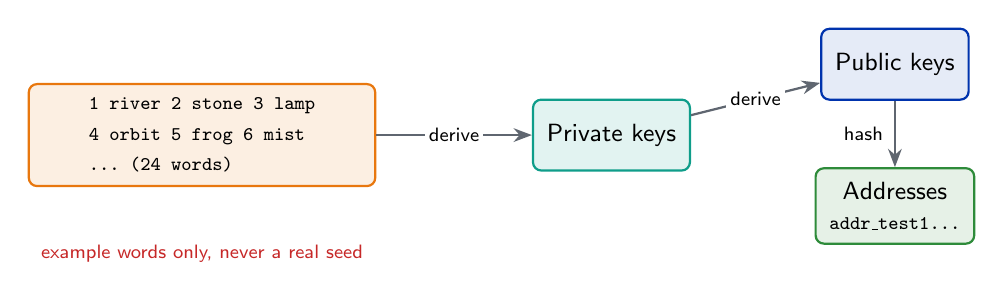
\begin{tikzpicture}
  \node[human,minimum width=4.4cm,align=left] (seed) at (0,0) {\ttfamily\scriptsize 1 river   2 stone   3 lamp\\\ttfamily\scriptsize 4 orbit   5 frog   6 mist\\\ttfamily\scriptsize \ldots\ (24 words)};
  \node[chain] (keys) at (5.2,0) {Private keys};
  \node[actor] (pubs) at (8.8,0.9) {Public keys};
  \node[good] (addr) at (8.8,-0.9) {Addresses\\\texttt{\scriptsize addr\_test1...}};
  \draw[flow] (seed) -- node[lbl]{derive} (keys);
  \draw[flow] (keys) -- node[lbl]{derive} (pubs);
  \draw[flow] (pubs) -- node[lbl,xshift=-4mm]{hash} (addr);
  \node[font=\sffamily\scriptsize,cRed] at (0,-1.5) {example words only, never a real seed};
\end{tikzpicture}
\caption{One mnemonic generates all keys and addresses. Everything flows one way: you cannot go from an address back to the mnemonic.}
\end{figure}

\begin{warningbox}{Never share your seed phrase}
Anyone who sees your seed phrase can recreate your keys and take everything, on every address, forever. No bank can reverse it. Rules for our team:
\begin{itemize}
  \item Never paste a mnemonic into chat, a ticket, a screenshot, or a Git commit.
  \item Keep it only in a local \code{.env} file that is listed in \code{.gitignore}, or in a password manager.
  \item For the hackathon, use \emph{throwaway test wallets} that hold only worthless test funds.
  \item Nobody legitimate (not a mentor, not a ``support agent'') will ever ask for it.
\end{itemize}
\end{warningbox}

\begin{shelfiebox}{Our wallets are server-side}
In Shelfie, our backend signs payments itself. The research notes describe a headless signer that reads a 24-word mnemonic from an environment variable (\code{.env}) instead of a browser wallet. That is convenient for agents, and it is exactly why the mnemonic must be a test-only throwaway wallet that never reaches Git.
\end{shelfiebox}

\section{Transactions}

A \term{transaction} (``tx'') is a signed instruction to change the ledger: ``move these funds from here to there''. It contains who spends what, who receives how much, a fee, and the signature(s) of the owner(s). The network checks the rules and, if valid, accepts it. Then the transaction gets its \term{transaction hash} (tx hash), which acts as its unique ID and receipt.

\begin{figure}[h]
\centering
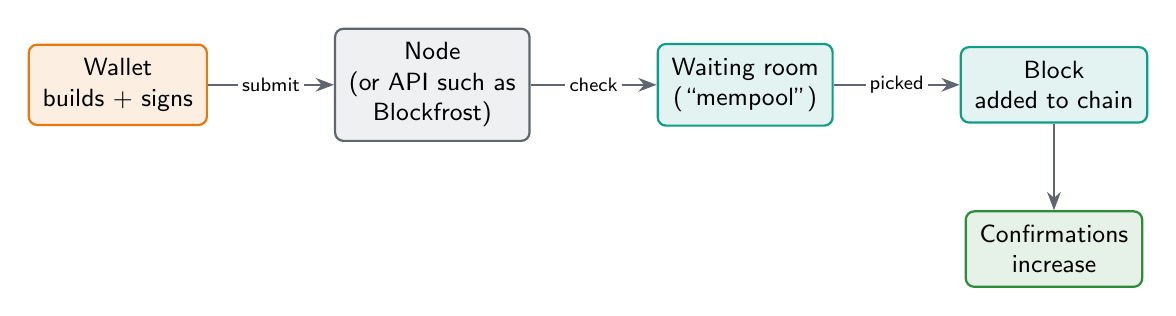
\begin{tikzpicture}[node distance=1.6cm]
  \node[human] (w) {Wallet\\builds + signs};
  \node[service,right=of w] (node) {Node\\(or API such as\\Blockfrost)};
  \node[chain,right=of node] (pool) {Waiting room\\(``mempool'')};
  \node[chain,right=of pool] (blk) {Block\\added to chain};
  \node[good,below=1.1cm of blk] (conf) {Confirmations\\increase};
  \draw[flow] (w) -- node[lbl]{submit} (node);
  \draw[flow] (node) -- node[lbl]{check} (pool);
  \draw[flow] (pool) -- node[lbl]{picked} (blk);
  \draw[flow] (blk) -- (conf);
\end{tikzpicture}
\caption{Life of a transaction: build and sign, submit, wait, be included in a block, then gain confirmations.}
\end{figure}

\begin{examplebox}{A simple payment}
Mia wants to pay worker Noor 4~ADA for a photo. Her wallet builds a transaction: ``Mia's funds $\rightarrow$ 4~ADA to Noor's address, fee $\approx 0.17$~ADA''. Mia's wallet signs it with her private key and sends it. A few seconds later it sits in a block. The tx hash can now be given to Noor, or to a judge, as proof.
\end{examplebox}

\section{Blocks and the chain}

Transactions are not added to the ledger one by one. Nodes collect many valid transactions and group them into a \term{block}. Each block contains:
\begin{itemize}
  \item a list of transactions,
  \item a timestamp (or slot number),
  \item the \textbf{hash of the previous block},
  \item its own hash.
\end{itemize}
Because each block includes the previous block's hash, the blocks form a \term{chain}. This is where the name ``blockchain'' comes from.

\begin{figure}[h]
\centering
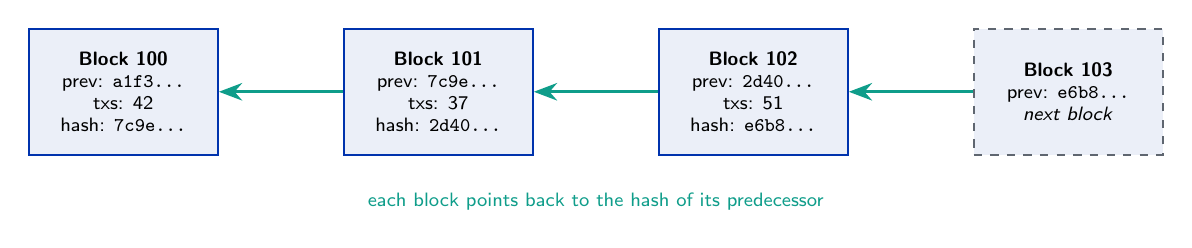
\begin{tikzpicture}
  \node[blk] (b1) at (0,0) {\textbf{Block 100}\\prev: \ttfamily a1f3\ldots\\txs: 42\\hash: \ttfamily 7c9e\ldots};
  \node[blk] (b2) at (4.0,0) {\textbf{Block 101}\\prev: \ttfamily 7c9e\ldots\\txs: 37\\hash: \ttfamily 2d40\ldots};
  \node[blk] (b3) at (8.0,0) {\textbf{Block 102}\\prev: \ttfamily 2d40\ldots\\txs: 51\\hash: \ttfamily e6b8\ldots};
  \node[blk,dashed,draw=cGrey] (b4) at (12.0,0) {\textbf{Block 103}\\prev: \ttfamily e6b8\ldots\\\textit{next block}};
  \draw[->,very thick,draw=cTeal] (b2.west) -- (b1.east);
  \draw[->,very thick,draw=cTeal] (b3.west) -- (b2.east);
  \draw[->,very thick,draw=cTeal] (b4.west) -- (b3.east);
  \node[font=\sffamily\scriptsize,cTeal] at (6,-1.4) {each block points back to the hash of its predecessor};
\end{tikzpicture}
\caption{A chain of blocks. The hashes shown are shortened examples.}
\end{figure}

\subsection{Why chaining makes history hard to change}
Suppose an attacker alters one old payment in Block~101. Block~101's content changes, so its hash changes. But Block~102 stored the \emph{old} hash of 101, so the link breaks. To hide the fraud, the attacker must also recompute Block~102, 103, and every later block, and then convince the majority of the network to accept this alternative history. The more blocks sit on top of a transaction, the more effort that takes.

\begin{figure}[h]
\centering
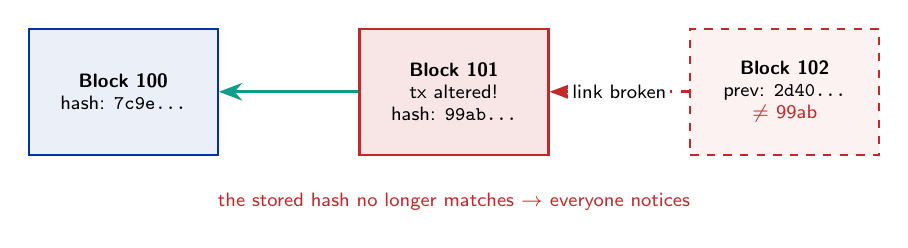
\begin{tikzpicture}
  \node[blk] (b1) at (0,0) {\textbf{Block 100}\\hash: \ttfamily 7c9e\ldots};
  \node[blk,fill=cRed!12,draw=cRed] (b2) at (4.2,0) {\textbf{Block 101}\\tx altered!\\hash: \ttfamily 99ab\ldots};
  \node[blk,fill=cRed!6,draw=cRed,dashed] (b3) at (8.4,0) {\textbf{Block 102}\\prev: \ttfamily 2d40\ldots\\ \textcolor{cRed}{$\neq$ 99ab}};
  \draw[->,very thick,draw=cTeal] (b2.west) -- (b1.east);
  \draw[->,very thick,draw=cRed,dashed] (b3.west) -- node[lbl]{link broken} (b2.east);
  \node[font=\sffamily\scriptsize,cRed] at (4.2,-1.4) {the stored hash no longer matches $\rightarrow$ everyone notices};
\end{tikzpicture}
\caption{Tampering with one block breaks the link in the next block.}
\end{figure}

\section{Consensus: how the network agrees}

If thousands of computers keep a copy, who decides which block comes next? The rules for agreeing are called \term{consensus}. Two major families exist.

\subsection{Proof of Work (PoW)}
Used by Bitcoin. Miners compete to solve a hard puzzle (guess a number so that the block's hash starts with many zeros). The winner adds the next block and gets a reward. The puzzle needs massive computing power and electricity, which makes cheating expensive.

\subsection{Proof of Stake (PoS)}
Used by Cardano (and Ethereum today). Instead of burning electricity, participants \emph{lock up} coins as a deposit, their \term{stake}. The protocol selects who creates the next block, with probability proportional to stake. Cheating risks the deposit and reputation, and honest work earns rewards.

\begin{table}[h]
\centering
\small
\begin{tabular}{@{}p{3.2cm}p{5.6cm}p{5.6cm}@{}}
\toprule
 & \textbf{Proof of Work} & \textbf{Proof of Stake}\\
\midrule
Scarce resource & computing power and electricity & locked coins (stake)\\
Who adds blocks & miners who win a puzzle & validators chosen by stake\\
Energy use & very high & low\\
Entry barrier & special hardware & coins (or delegate to a pool)\\
Example & Bitcoin & Cardano, Ethereum\\
Typical block time & Bitcoin: about 10 minutes & Cardano: about 20 seconds\\
\bottomrule
\end{tabular}
\caption{PoW versus PoS in one view. Block times are approximate.}
\end{table}

\begin{analogybox}{Lottery with deposits}
PoS is like a raffle where every ticket is a coin you have locked as a deposit. The more tickets you hold, the more often you are drawn to write the next page of the notebook. If you cheat, your deposit is at risk.
\end{analogybox}

\subsection{Forks}
Sometimes two valid blocks appear almost at the same time and the chain briefly splits into two branches (a \term{fork}). The protocol's rule (for example, ``follow the longest valid chain'') quickly makes everybody prefer one branch. Transactions only in the abandoned branch go back to the waiting room and are normally included again. This is why a freshly included transaction is not yet ``final''.

\section{Finality and confirmations}

A transaction is \term{confirmed} once it is in a block, and each new block built on top is another \term{confirmation}. The deeper it is buried, the less likely it is that a fork will remove it. \term{Finality} means the point at which reversal is practically impossible.

\begin{figure}[h]
\centering
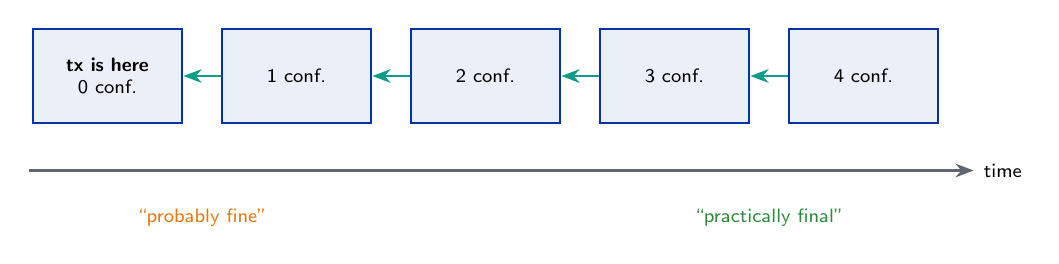
\begin{tikzpicture}
  \foreach \i/\c in {0/cBlue,1/cBlue,2/cBlue,3/cBlue,4/cBlue}{
    \node[blk,minimum width=1.9cm,minimum height=1.2cm,fill=\c!8,draw=\c] (b\i) at (2.4*\i,0) {};
  }
  \node[font=\sffamily\scriptsize,align=center] at (b0) {\textbf{tx is here}\\0 conf.};
  \node[font=\sffamily\scriptsize] at (b1) {1 conf.};
  \node[font=\sffamily\scriptsize] at (b2) {2 conf.};
  \node[font=\sffamily\scriptsize] at (b3) {3 conf.};
  \node[font=\sffamily\scriptsize] at (b4) {4 conf.};
  \foreach \i/\j in {1/0,2/1,3/2,4/3}{\draw[->,thick,draw=cTeal] (b\i.west) -- (b\j.east);}
  \draw[->,thick,draw=cGrey] (-1,-1.2) -- (11,-1.2) node[right,font=\sffamily\scriptsize]{time};
  \node[font=\sffamily\scriptsize,cOrange] at (1.2,-1.8) {``probably fine''};
  \node[font=\sffamily\scriptsize,cGreen] at (8.4,-1.8) {``practically final''};
\end{tikzpicture}
\caption{Each block added on top of the transaction's block adds one confirmation.}
\end{figure}

\begin{warningbox}{``Submitted'' is not ``confirmed''}
A node accepting your transaction only means it entered the waiting room. For a payment you must wait until it is in a block, and ideally a few blocks deep. Our research notes also warn: if a payment call times out or the connection drops after ``sending'', the payment may \emph{still} settle later. Always check the explorer before sending again, otherwise you may pay twice.
\end{warningbox}

\begin{shelfiebox}{Why our payout queue reconciles}
The design stores a metadata tag on every payout transaction and, after a crash or timeout, looks the chain up for that tag before ever retrying. Exactly one payout per task is the rule. The mechanism and its states are described in the Shelfie architecture chapters.
\end{shelfiebox}

\section{Fees}

Using the network costs a small \term{transaction fee}. Fees pay the people who run the infrastructure and discourage spam. On Cardano the fee depends mostly on the transaction's \emph{size in bytes} (plus script execution if scripts are used), and is typically a fraction of an ADA; the team's runbook mentions about 0.17 ADA per payment. The sender pays the fee on top of the amount sent.

Different chains price fees differently: some are almost free, some become very expensive when busy. Predictable, low fees are what makes small machine payments (a few cents) practical.

\section{Tokens and stablecoins}

The chain's own currency (for Cardano: ADA) is the \term{native coin}. Besides it, chains can carry other \term{tokens}: digital items that represent value, points, access rights, or a real-world currency.

A \term{stablecoin} is a token designed to keep a stable value, usually 1 token $\approx$ 1 US dollar. This is important for commerce: a shop does not want its price to move 10\,\% between the order and the payment.

\begin{table}[h]
\centering
\small
\begin{tabular}{@{}p{3.3cm}p{5.4cm}p{5.6cm}@{}}
\toprule
 & \textbf{Native coin (ADA)} & \textbf{Stablecoin (e.g.\ USDM)}\\
\midrule
Value & floats with the market & aims at a fixed peg (dollar)\\
Needed for fees & \yes\ always & \no\ fees still need ADA\\
Good for & fees, staking, security & stable prices\\
On testnet & tADA, free & test version (tUSDM), free\\
\bottomrule
\end{tabular}
\caption{Coin versus stablecoin.}
\end{table}

\begin{shelfiebox}{We price in tADA}
The design decision (ADR-03) is to price the verifier fee and worker payouts in tADA, not in a test stablecoin. The reason is that two incompatible test-stablecoin tokens exist (the SDK one and the one from the Masumi dispenser), so a wallet funded with one cannot pay a route priced in the other. Plain tADA avoids this trap.
\end{shelfiebox}

\section{Smart contracts (a first look)}

A \term{smart contract} is a program stored on the blockchain that runs automatically when its conditions are met and enforces rules without a middleman. Typical rules: ``release the money only when both parties signed'' or ``refund the buyer if no result arrives within a time limit''. Because the program's code and the ledger are shared, nobody can quietly change the rules afterwards.

\begin{analogybox}{The vending machine}
A vending machine is a contract: put in the coins, press the button, and the product drops. No cashier is needed, and the machine follows the same rule for everybody. A smart contract is a vending machine for agreements.
\end{analogybox}

This is only the intro. How Cardano runs contracts (validators, datum, redeemer) is explained in Chapter~2. For Shelfie, an important point: Masumi's \emph{escrow} (money locked until the job result is delivered) is a smart-contract mechanism that we use through the Masumi service; we do not write our own contract for the MVP.

\section{Public explorers}

A \term{block explorer} is a website that lets anyone search the public ledger: by transaction hash, address, or block. It is the ``receipt viewer'' of a blockchain. Because chains are public, anyone (a judge, a worker, a teammate) can open the same page and see the same facts, without having to trust our app.

\begin{figure}[h]
\centering
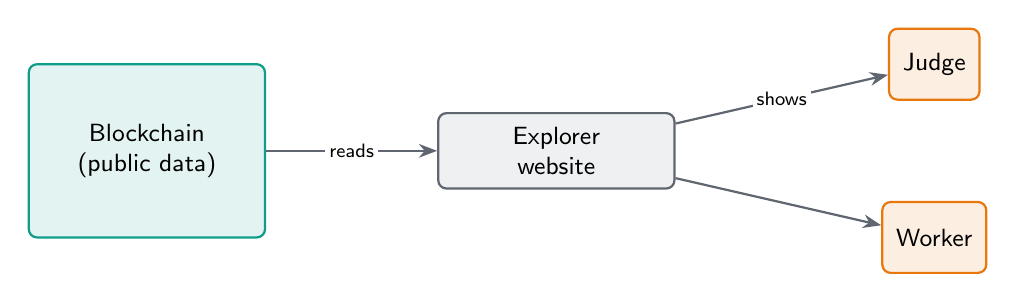
\begin{tikzpicture}
  \node[chain,minimum width=3cm,minimum height=2.2cm] (chain) at (0,0) {Blockchain\\(public data)};
  \node[service,minimum width=3cm] (exp) at (5.2,0) {Explorer\\website};
  \node[human] (jud) at (10,1.1) {Judge};
  \node[human] (wk) at (10,-1.1) {Worker};
  \draw[flow] (chain) -- node[lbl]{reads} (exp);
  \draw[flow] (exp) -- node[lbl]{shows} (jud);
  \draw[flow] (exp) -- (wk);
\end{tikzpicture}
\caption{An explorer turns raw ledger data into pages anyone can open and share as a link.}
\end{figure}

On Cardano the explorer we use is Cardanoscan (preprod version); Chapter~2 shows how to read a transaction page.

\section{Testnets and mainnet}

The real network, where coins have real money value, is the \term{mainnet}. A \term{testnet} is a copy of the technology with worthless test coins, built for developers to experiment without risking money. You can get test coins for free from a \term{faucet}, a website that hands them out.

\begin{table}[h]
\centering
\small
\begin{tabular}{@{}p{3.4cm}p{5.5cm}p{5.5cm}@{}}
\toprule
 & \textbf{Mainnet} & \textbf{Testnet}\\
\midrule
Coins have value & \yes & \no\\
Mistakes cost money & \yes & \no\\
Faucet available & \no & \yes\\
Used for & real products & development, demos, hackathons\\
Example addresses (Cardano) & \texttt{addr1...} & \texttt{addr\_test1...}\\
\bottomrule
\end{tabular}
\caption{Mainnet versus testnet.}
\end{table}

\begin{warningbox}{Check which network you are on}
Mixing networks is a classic mistake: a testnet address cannot receive mainnet money, and tools sometimes default to mainnet. The runbooks warn that the Sokosumi MCP server defaults to mainnet, so always confirm the network is \emph{preprod} before paying. All hackathon money is play money, and we state our amounts as tADA.
\end{warningbox}

\section{Why use a blockchain for payments between machines?}

Imagine a software agent that needs to buy a service from another agent, at 3 a.m., for 0.2~EUR, with an unknown counterpart across the world. Compare this with normal card or bank payments.

\begin{table}[h]
\centering
\small
\begin{tabularx}{\textwidth}{@{}p{3.6cm}XX@{}}
\toprule
 & \textbf{Card or bank transfer} & \textbf{Blockchain payment}\\
\midrule
Needs a bank account & \yes\ (a human or company must open it) & \no\ a key pair is enough\\
Programmable by software & limited, via bank APIs and approvals & \yes\ build, sign, submit by code\\
Works for tiny amounts & often not (fixed fees) & \yes\ if fees are small\\
Availability & business hours, borders & 24/7, global\\
Public receipt & \no\ private to the parties & \yes\ tx hash anybody can verify\\
Reversible (chargeback) & \yes & \no\ final\\
Escrow with machine rules & hard & \yes\ via smart contracts\\
\bottomrule
\end{tabularx}
\caption{Why machines (and Shelfie) prefer on-chain payments.}
\end{table}

The trade-off is real: finality means mistakes cannot be reversed, and tools are younger. But for software agents paying each other, \textbf{no account, programmable, public receipt} is exactly what is needed.

\begin{shelfiebox}{What we gain in the demo}
Judges will not need to trust our slides. Every verifier fee and every worker payout is a real tADA transaction on Cardano preprod that they can open with a link on Cardanoscan. That public receipt is our strongest piece of evidence.
\end{shelfiebox}

\begin{keypoints}
\begin{itemize}
  \item A \textbf{ledger} lists who owns what; a \textbf{blockchain} is a ledger copied across many computers with no single owner.
  \item A \textbf{hash} is a fixed-size fingerprint; changing the input by one character changes it completely.
  \item A \textbf{private key} signs; the matching \textbf{public key} verifies. Whoever has the private key (or the seed phrase) controls the funds.
  \item \textbf{Never share a seed phrase}; use throwaway wallets with test funds only.
  \item A \textbf{transaction} is a signed change to the ledger, identified by its tx hash; blocks are linked by hashes, so history is hard to rewrite.
  \item Consensus is how the network agrees: \textbf{PoW} uses computing power, \textbf{PoS} (Cardano) uses staked coins.
  \item Confirmations grow with each new block; ``submitted'' does not mean ``final''.
  \item Fees are small and paid in the native coin; stablecoins keep a steady price; smart contracts enforce rules automatically.
  \item Explorers make the ledger readable; testnets use free, worthless coins; mainnet is real money.
  \item Machines like blockchains: no bank account, programmable, public receipts.
\end{itemize}
\end{keypoints}

\begin{quizbox}
\begin{enumerate}
  \item You change a single letter in a message and hash it again. What happens to the hash, and why does this help to detect fraud?
  \item Who can create a valid signature, and who can verify it?
  \item Why can a stranger who finds your 24-word mnemonic empty all your addresses?
  \item Why does altering an old block break all blocks after it?
  \item Name one advantage of Proof of Stake over Proof of Work, and what Cardano uses.
  \item Your payout call timed out. Why should you check the explorer before sending again?
\end{enumerate}
{\footnotesize\color{cGrey}\textbf{Answers.} (1) It changes completely and unpredictably; stored hashes then no longer match. (2) Only the holder of the private key signs; anybody with the public key verifies. (3) The mnemonic regenerates every private key. (4) The next block stores the old block's hash, so the link no longer matches. (5) Far lower energy use; Cardano uses Proof of Stake. (6) The first payment may still settle, and a retry would pay twice.}
\end{quizbox}

\chapter{Cardano}

\section*{Why this matters for us}
The track is called ``Agentic Commerce on Cardano''. Every payment in Shelfie (the verifier fee, the worker payout, the escrow around the brand's job) is a Cardano transaction. If the team understands Cardano's \emph{UTXO} model, two of the most common bugs (``why does my wallet say no funds?'' and ``why can't two payments leave one wallet at once?'') become obvious instead of mysterious. This chapter explains what Cardano is, how its money works, which tools we use to talk to it, and finally exactly which parts we touch in our project.

\section{What is Cardano?}

\term{Cardano} is a public, proof-of-stake blockchain (see Chapter~1) with its own coin, \term{ADA}. It was built with a research-driven approach and is known for formal methods, low and predictable fees, and a ledger model called \emph{extended UTXO} that we explain in detail below.

\begin{table}[h]
\centering
\small
\begin{tabular}{@{}p{4.2cm}p{10.2cm}@{}}
\toprule
\textbf{Property} & \textbf{On Cardano}\\
\midrule
Consensus & Ouroboros, a Proof-of-Stake protocol\\
Native coin & ADA (smallest unit: lovelace)\\
Ledger model & extended UTXO (eUTXO)\\
Smart contract languages & Plutus (Haskell-based), Aiken, and others that compile to the same on-chain code\\
Native tokens & built into the ledger; no contract needed to create or send them\\
TypeScript tooling & Mesh, Lucid Evolution, Evolution SDK (used by the x402 template)\\
\bottomrule
\end{tabular}
\caption{Cardano at a glance.}
\end{table}

\section{ADA and lovelace}

The coin is called \term{ADA}. Like cents are to euros, the smallest unit is called a \term{lovelace}:
\[
1\ \text{ADA} = 1{,}000{,}000\ \text{lovelace}.
\]
Software works with whole numbers of lovelace (no decimals, no rounding errors); humans read ADA. Our design contracts use lovelace, and our prose uses ADA.

\begin{examplebox}{Converting between ADA and lovelace}
\begin{center}
\small
\begin{tabular}{rcr}
\toprule
\textbf{ADA} & & \textbf{lovelace}\\
\midrule
1 ADA & = & 1{,}000{,}000\\
2 ADA (a typical x402 price in the runbook) & = & 2{,}000{,}000\\
0.17 ADA (typical fee) & = & 170{,}000\\
0.5 ADA & = & 500{,}000\\
5 ADA & = & 5{,}000{,}000\\
\bottomrule
\end{tabular}
\end{center}
To go from ADA to lovelace, multiply by one million; to go back, divide by one million. In a code field such as \code{amount: "5000000"} that means \emph{5 ADA}, not five million ADA.
\end{examplebox}

\begin{warningbox}{Off by a factor of a million}
A classic bug: writing \code{5} when you meant 5~ADA sends 5 lovelace (0.000005 ADA), which is below the minimum and will be rejected. Always check the unit in a field name or doc before using a number.
\end{warningbox}

\begin{shelfiebox}{tADA, not ADA}
On the preprod test network, the coin is named \term{tADA} (test ADA). It behaves exactly like ADA but has no value. All Shelfie prices and payouts are in tADA. Any euro value in the pitch is illustrative only.
\end{shelfiebox}

\section{Ouroboros and stake pools}

\term{Ouroboros} is Cardano's Proof-of-Stake protocol. Time is cut into short \term{slots} (one second each) grouped into \term{epochs} (five days). For each slot a \term{stake pool} is chosen at random, weighted by the amount of ADA staked with it, and that pool creates the block. A pool is run by a \term{stake pool operator}.

\subsection{Delegation}
You do not need to run a pool to take part. You can \term{delegate} your stake to a pool: your coins stay in your wallet, under your control, and are never sent anywhere; you only point their voting weight to a pool and receive a share of the rewards. Delegation is a mainnet topic and does not matter for the hackathon; it is mentioned here so that the words are familiar.

\begin{figure}[h]
\centering
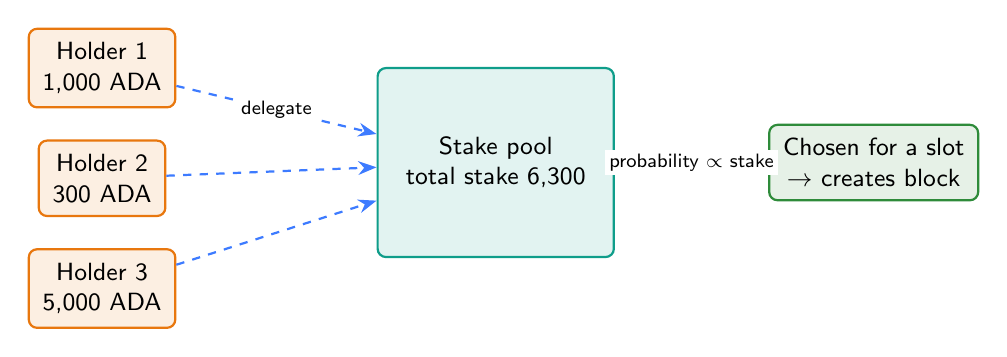
\begin{tikzpicture}
  \node[human] (h1) at (0,1.2) {Holder 1\\1,000 ADA};
  \node[human] (h2) at (0,-0.2) {Holder 2\\300 ADA};
  \node[human] (h3) at (0,-1.6) {Holder 3\\5,000 ADA};
  \node[chain,minimum width=3cm,minimum height=2.4cm] (pool) at (5,0) {Stake pool\\total stake 6,300};
  \node[good] (blk) at (9.8,0) {Chosen for a slot\\$\rightarrow$ creates block};
  \draw[data] (h1) -- node[lbl]{delegate} (pool);
  \draw[data] (h2) -- (pool);
  \draw[data] (h3) -- (pool);
  \draw[flow] (pool) -- node[lbl]{probability $\propto$ stake} (blk);
\end{tikzpicture}
\caption{Delegation: holders keep their coins and lend their weight to a pool. The numbers are made up.}
\end{figure}

\section{The eUTXO model, step by step}

This is the most important concept of the chapter. Take your time.

\subsection{Two ways to keep a ledger}
There are two common ways to record who owns what:

\begin{description}
  \item[Account model.] Each address has a balance, like a bank account: ``Mia: 15 ADA''. A payment subtracts from one balance and adds to another. Ethereum works this way.
  \item[UTXO model.] There are no balances. The ledger holds a set of individual coin ``chunks'' called \term{UTXOs}. Your ``balance'' is the sum of the chunks you can spend. Bitcoin and Cardano work this way.
\end{description}

\term{UTXO} stands for \emph{Unspent Transaction Output}. An \emph{output} is created by a transaction and sits on the ledger, owned by an address, until another transaction \emph{spends} it. A UTXO can only be spent \emph{whole and once}.

\begin{analogybox}{Banknotes and coins in a wallet}
Your leather wallet has a 10-euro note and a 5-euro note. You do not own ``15 euros in an account''; you own two physical items that add up to 15. To pay 4 euros you hand over the 10-euro note. The shop gives you 6 euros back as \emph{change}. The note you gave is gone (spent); you now hold new items: the 5-euro note and the 6 euros change. UTXOs work exactly like this.
\end{analogybox}

\subsection{Inputs and outputs}
Every transaction has:
\begin{itemize}
  \item \textbf{Inputs:} the UTXOs it \emph{consumes} (destroys). Each must be owned by someone who signs, or locked by a script that agrees.
  \item \textbf{Outputs:} the new UTXOs it \emph{creates}, each with an address and an amount.
  \item A \textbf{fee} and optional extras (metadata, scripts).
\end{itemize}
The golden rule:
\[
\sum \text{inputs} \;=\; \sum \text{outputs} \;+\; \text{fee}.
\]
Nothing is created and nothing vanishes; it is only re-cut into new pieces.

\begin{figure}[h]
\centering
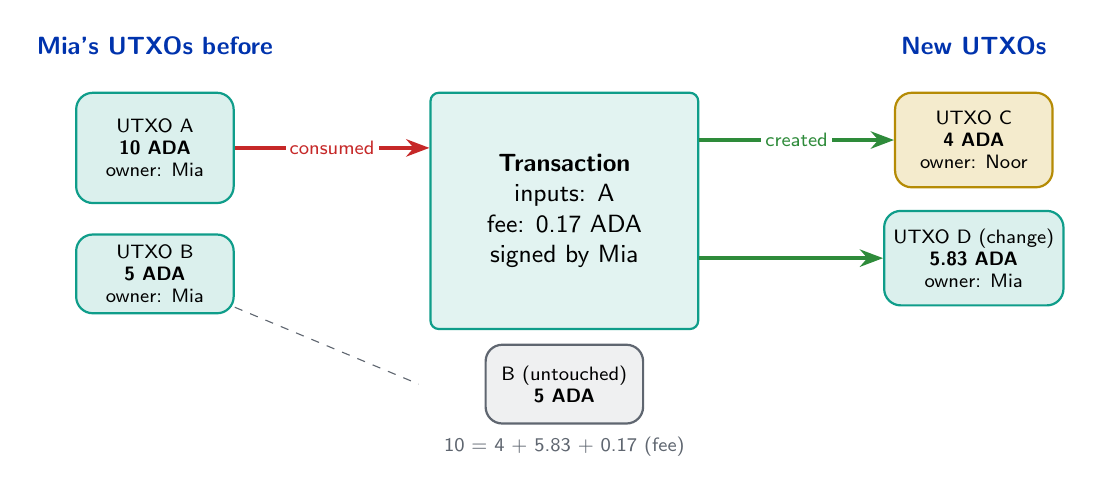
\begin{tikzpicture}
  % before
  \node[font=\sffamily\bfseries\small,cBlue] at (1.2,3.3) {Mia's UTXOs before};
  \node[utxo,minimum height=1.4cm] (a) at (1.2,2.0) {UTXO A\\\textbf{10 ADA}\\owner: Mia};
  \node[utxo,minimum height=1.0cm] (b) at (1.2,0.4) {UTXO B\\\textbf{5 ADA}\\owner: Mia};
  % tx
  \node[chain,minimum width=3.4cm,minimum height=3cm] (tx) at (6.4,1.2) {\textbf{Transaction}\\inputs: A\\fee: 0.17 ADA\\signed by Mia};
  \draw[->,very thick,draw=cRed] (a) -- node[lbl,text=cRed]{consumed} (tx.west |- a);
  % after
  \node[font=\sffamily\bfseries\small,cBlue] at (11.6,3.3) {New UTXOs};
  \node[utxo,fill=cGold!20,draw=cGold!90!black,minimum height=1.2cm] (o1) at (11.6,2.1) {UTXO C\\\textbf{4 ADA}\\owner: Noor};
  \node[utxo,minimum height=1.2cm] (o2) at (11.6,0.6) {UTXO D (change)\\\textbf{5.83 ADA}\\owner: Mia};
  \draw[->,very thick,draw=cGreen] (tx.east |- o1) -- node[lbl,text=cGreen]{created} (o1);
  \draw[->,very thick,draw=cGreen] (tx.east |- o2) -- (o2);
  \node[utxo,draw=cGrey,fill=cGrey!10,minimum height=1cm] at (6.4,-1.0) {B (untouched)\\\textbf{5 ADA}};
  \draw[dashed,draw=cGrey] (b) -- (4.55,-1.0);
  \node[font=\sffamily\scriptsize,cGrey] at (6.4,-1.8) {10 = 4 + 5.83 + 0.17 (fee)};
\end{tikzpicture}
\caption{Mia pays Noor 4 ADA. Input A (10 ADA) is destroyed; two new outputs appear: 4 ADA for Noor and 5.83 ADA change back to Mia; 0.17 ADA is the fee. UTXO B is not used.}
\end{figure}

\subsection{Why there is always a change output}
Because a UTXO can only be spent whole, you cannot ``take 4 out of the 10''. Instead you consume all 10 and create \emph{two} outputs: one for the recipient and one that sends the rest back to yourself (the \term{change output}). A wallet does this automatically. If you forget to add a change output in your own code, the leftover ADA is swallowed by the fee.

\begin{warningbox}{Forgetting the change}
If the inputs add up to 10~ADA but your outputs only add up to 4~ADA, the transaction is invalid (fee too high) or, in a hand-built transaction, you would donate the remaining 5.83~ADA to the fee. Always check that inputs, outputs and fee balance.
\end{warningbox}

\subsection{Worked numeric example}

\begin{examplebox}{Mia pays Noor, twice}
\textbf{Start.} Mia's wallet holds two UTXOs: A = 10~ADA and B = 5~ADA. Her ``balance'' is 15~ADA. Fee for each payment: 0.17~ADA (illustrative).

\medskip
\textbf{Payment 1: 4 ADA to Noor.} The wallet picks A (it is big enough).
\begin{center}
\small
\begin{tabular}{@{}lrl@{}}
\toprule
 & ADA & \\
\midrule
Input A & 10.00 & \\
Output to Noor (new UTXO C) & 4.00 & \\
Change to Mia (new UTXO D) & 5.83 & \\
Fee & 0.17 & \\
\midrule
Check: 4.00 + 5.83 + 0.17 & 10.00 & equals the input \\
\bottomrule
\end{tabular}
\end{center}
Mia now owns B (5.00) and D (5.83): balance 10.83 ADA.

\medskip
\textbf{Payment 2: 10 ADA to Noor.} Neither B (5.00) nor D (5.83) is large enough on its own, so the wallet uses \emph{both} as inputs.
\begin{center}
\small
\begin{tabular}{@{}lrl@{}}
\toprule
 & ADA & \\
\midrule
Inputs B + D & 10.83 & \\
Output to Noor & 10.00 & \\
Change to Mia & 0.66 & \\
Fee & 0.17 & \\
\midrule
Check: 10.00 + 0.66 + 0.17 & 10.83 & equals the inputs \\
\bottomrule
\end{tabular}
\end{center}
Mia keeps one UTXO of 0.66 ADA. (Whether 0.66 ADA is allowed as a lone output depends on the minimum-ADA rule, see below; the example only illustrates the arithmetic.)
\end{examplebox}

\begin{figure}[h]
\centering
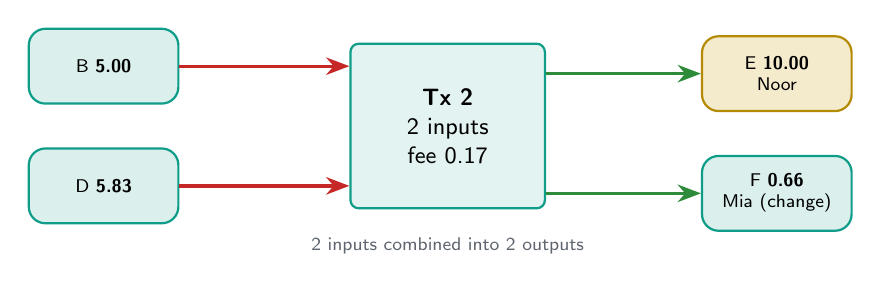
\begin{tikzpicture}[scale=0.95,transform shape]
  \node[utxo] (b) at (0,1.0) {B\ \textbf{5.00}};
  \node[utxo] (d) at (0,-0.6) {D\ \textbf{5.83}};
  \node[chain,minimum width=2.6cm,minimum height=2.2cm] (tx) at (4.6,0.2) {\textbf{Tx 2}\\2 inputs\\fee 0.17};
  \draw[->,very thick,draw=cRed] (b) -- (tx.west |- b);
  \draw[->,very thick,draw=cRed] (d) -- (tx.west |- d);
  \node[utxo,fill=cGold!20,draw=cGold!90!black] (e) at (9,0.9) {E\ \textbf{10.00}\\Noor};
  \node[utxo] (f) at (9,-0.7) {F\ \textbf{0.66}\\Mia (change)};
  \draw[->,very thick,draw=cGreen] (tx.east |- e) -- (e);
  \draw[->,very thick,draw=cGreen] (tx.east |- f) -- (f);
  \node[font=\sffamily\scriptsize,cGrey] at (4.6,-1.4) {2 inputs combined into 2 outputs};
\end{tikzpicture}
\caption{Combining small UTXOs: Payment~2 consumes B and D together.}
\end{figure}

\subsection{The ledger is a set of unspent outputs}
It helps to picture the whole chain as a big shelf of UTXOs. A transaction removes some items from the shelf (inputs) and puts new ones on it (outputs). An item that has been removed can never be used again. This is why double spending is impossible: the second attempt to spend the same UTXO finds it already gone.

\begin{figure}[h]
\centering
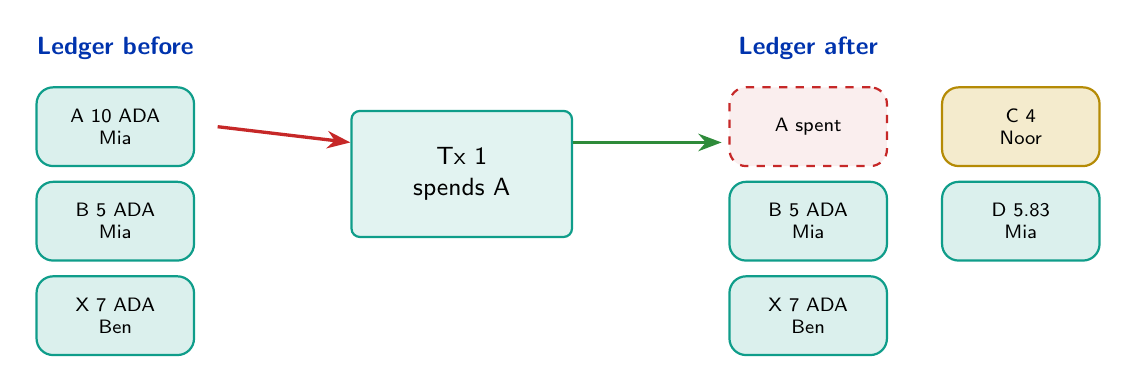
\begin{tikzpicture}
  \node[font=\sffamily\bfseries\small,cBlue] at (1.6,3.1) {Ledger before};
  \node[utxo] at (1.6,2.1) {A\ 10 ADA\\Mia};
  \node[utxo] at (1.6,0.9) {B\ 5 ADA\\Mia};
  \node[utxo] at (1.6,-0.3) {X\ 7 ADA\\Ben};
  \node[chain,minimum width=2.8cm,minimum height=1.6cm] (tx) at (6,1.5) {Tx 1\\spends A};
  \draw[->,very thick,draw=cRed] (2.9,2.1) -- (tx.west |- 0,1.9);
  \node[font=\sffamily\bfseries\small,cBlue] at (10.4,3.1) {Ledger after};
  \node[utxo,draw=cRed,fill=cRed!8,dashed] at (10.4,2.1) {A\ spent};
  \node[utxo] at (10.4,0.9) {B\ 5 ADA\\Mia};
  \node[utxo] at (10.4,-0.3) {X\ 7 ADA\\Ben};
  \node[utxo,fill=cGold!20,draw=cGold!90!black] at (13.1,2.1) {C\ 4\\Noor};
  \node[utxo] at (13.1,0.9) {D\ 5.83\\Mia};
  \draw[->,very thick,draw=cGreen] (tx.east |- 0,1.9) -- (9.3,1.9);
\end{tikzpicture}
\caption{Each transaction rewrites a small part of the shelf of unspent outputs. A spent UTXO cannot be used again.}
\end{figure}

\subsection{Account model versus eUTXO}

\begin{table}[h]
\centering
\small
\begin{tabularx}{\textwidth}{@{}p{3.5cm}XX@{}}
\toprule
 & \textbf{Account model (e.g.\ Ethereum)} & \textbf{(e)UTXO model (Cardano)}\\
\midrule
State is & balance per account & set of unspent outputs\\
A payment & subtracts and adds balances & consumes inputs, creates outputs\\
Change output & not needed & needed\\
Two payments at once from one wallet & usually ok (ordered by a nonce) & can conflict if they pick the same UTXO\\
Fee known before sending & only approximately & exact (depends on tx size)\\
Failed tx still costs fee & often yes & mostly no: invalid txs are rejected before inclusion\\
Smart contract state & stored inside the contract & carried in each UTXO's datum\\
Mental picture & bank account & banknotes in a wallet\\
\bottomrule
\end{tabularx}
\caption{Account model versus eUTXO.}
\end{table}

\begin{shelfiebox}{One wallet cannot pay twice at the same time}
The x402 runbook warns: ``one wallet cannot pay concurrently (the first UTxO is the nonce)''. Two parallel payments from the same wallet may pick the same UTXO as input, and the second one fails because that UTXO is already spent. This is why our design uses \emph{separate} wallets (W-VBUY, W-PAY, W-SELL) and a \emph{serial queue per wallet} (one send at a time, ADR-08). The throughput limit becomes the confirmation latency, about 20--60 seconds per check.
\end{shelfiebox}

\section{Extended UTXO: datum, redeemer, validator}

So far, every UTXO was owned by a key: only its owner's signature can spend it. The ``extended'' part of eUTXO allows a UTXO to be locked by a \emph{script} instead. Three ingredients appear.

\begin{description}
  \item[Validator (script).] A small program attached to an address (a \term{script address}). It decides whether a transaction may spend a UTXO sitting at that address. It answers only \emph{yes} or \emph{no}.
  \item[Datum.] Data stored \emph{inside the locked UTXO}, such as ``buyer = Bea, seller = Sam, deadline = Friday 18:00''. It is the state of the agreement.
  \item[Redeemer.] Data provided \emph{by the spender} in the new transaction, such as ``action = Release'' or ``action = Refund''. It is the argument with which one tries to unlock.
\end{description}

The validator receives the datum, the redeemer and the transaction context (who signed, what outputs are created, what time it is) and returns allow or deny.

\begin{figure}[h]
\centering
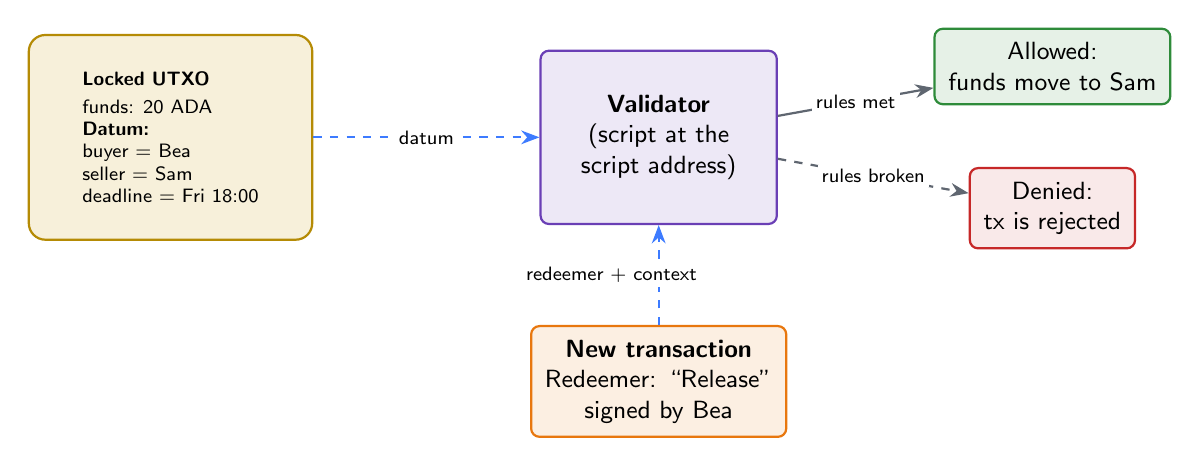
\begin{tikzpicture}
  \node[utxo,minimum width=3.6cm,minimum height=2.6cm,fill=cGold!15,draw=cGold!90!black,align=left] (u) at (0,0)
    {\textbf{Locked UTXO}\\[2pt]funds: 20 ADA\\\textbf{Datum:}\\buyer = Bea\\seller = Sam\\deadline = Fri 18:00};
  \node[agent,minimum width=3cm,minimum height=2.2cm] (v) at (6.2,0) {\textbf{Validator}\\(script at the\\script address)};
  \node[human,minimum width=3cm] (tx) at (6.2,-3.1) {\textbf{New transaction}\\Redeemer: ``Release''\\signed by Bea};
  \node[good] (ok) at (11.2,0.9) {Allowed:\\funds move to Sam};
  \node[bad] (no) at (11.2,-0.9) {Denied:\\tx is rejected};
  \draw[data] (u) -- node[lbl]{datum} (v);
  \draw[data] (tx) -- node[lbl,xshift=-6mm]{redeemer + context} (v);
  \draw[flow] (v) -- node[lbl]{rules met} (ok);
  \draw[flow,dashed] (v) -- node[lbl]{rules broken} (no);
\end{tikzpicture}
\caption{A validator checks datum, redeemer and the transaction before allowing the locked UTXO to be spent.}
\end{figure}

\begin{analogybox}{The safety-deposit box}
The locked UTXO is a deposit box at the bank. The \emph{datum} is the label with the agreement written on it. The \emph{redeemer} is what you say when you arrive: ``I am here to collect''. The \emph{validator} is the bank clerk who checks your papers against the label. No clerk can be bribed or changed: it is code that runs the same way for everybody.
\end{analogybox}

\subsection{Why this design matters}
Because the validator runs on a transaction you have already built, you can predict the result before sending: if the check fails, the transaction is simply rejected. No surprises, deterministic costs. This is one of Cardano's selling points.

\begin{examplebox}{A tiny escrow}
Bea wants to buy a result from Sam for 20~ADA.
\begin{enumerate}
  \item \textbf{Lock:} Bea sends 20 ADA to the script address with the datum \{buyer: Bea, seller: Sam, deadline: Friday 18:00\}.
  \item \textbf{Release:} when Sam delivers, a transaction with redeemer \emph{Release}, signed by Bea (or by an agreed party), spends the UTXO and creates an output of 20 ADA to Sam.
  \item \textbf{Refund:} if the deadline has passed and Sam never delivered, Bea can spend the UTXO with redeemer \emph{Refund} and gets the 20 ADA back.
\end{enumerate}
The script enforces both outcomes. Nobody needs to trust a middleman.
\end{examplebox}

\begin{figure}[h]
\centering
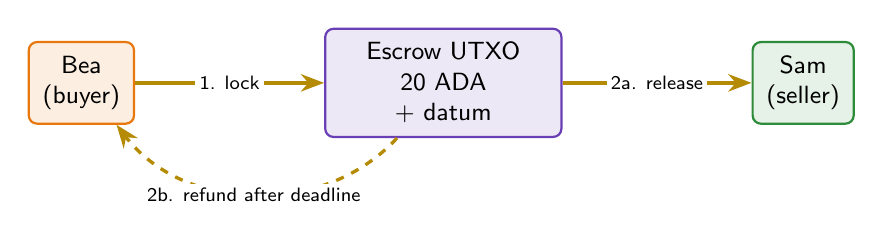
\begin{tikzpicture}[node distance=2.2cm]
  \node[human] (bea) {Bea\\(buyer)};
  \node[agent,right=2.4cm of bea,minimum width=3cm] (esc) {Escrow UTXO\\20 ADA\\+ datum};
  \node[good,right=2.4cm of esc] (sam) {Sam\\(seller)};
  \draw[pay] (bea) -- node[lbl]{1. lock} (esc);
  \draw[pay] (esc) -- node[lbl]{2a. release} (sam);
  \draw[pay,dashed] (esc) to[bend left=50] node[lbl]{2b. refund after deadline} (bea);
\end{tikzpicture}
\caption{Escrow: the money waits in the script until the job is done or the deadline passes.}
\end{figure}

\begin{shelfiebox}{Escrow comes from Masumi}
Our MVP does not write its own validator. The brand's fee for the lead agent is held in a \emph{Masumi escrow} (a ready-made contract, used through the Masumi Payment Service). After a worker's photo has passed our verifier, the engine pays the worker with a plain transfer from W-PAY. Writing a custom Aiken contract is only a possible stretch idea.
\end{shelfiebox}

\subsection{Plutus and Aiken}
Validators are written in a smart-contract language and compiled to a low-level on-chain format.
\begin{itemize}
  \item \term{Plutus}: Cardano's original contract platform, based on Haskell.
  \item \term{Aiken}: a newer, simpler language designed for validators, with its own CLI. The Mesh docs have a ``first validator'' guide covering datum, redeemer and signatures.
\end{itemize}
The off-chain code (building and submitting transactions) is usually written in TypeScript with libraries such as Mesh or Lucid Evolution, while the \emph{on-chain} part is the validator. We reuse existing on-chain contracts and write only off-chain TypeScript. The research notes rate writing and debugging our own Aiken validator as a medium-high to high effort, so it is not in the MVP.

\section{Native tokens}

On Cardano, tokens other than ADA are \term{native assets}: the ledger itself knows how to hold and move them, just like ADA. You do \emph{not} need a smart contract to create, hold or send such a token. A native token is identified by two parts:
\begin{itemize}
  \item the \term{policy ID}: a hash identifying the minting rules,
  \item the \term{asset name}: a short label within that policy.
\end{itemize}
A UTXO can carry ADA and several kinds of native tokens at once.

\begin{figure}[h]
\centering
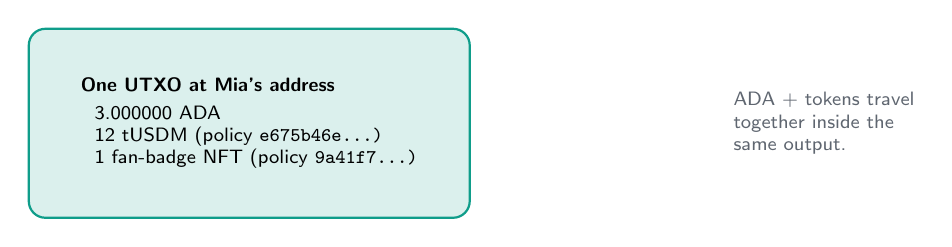
\begin{tikzpicture}
  \node[utxo,minimum width=5.6cm,minimum height=2.4cm,align=left] (u) at (0,0)
    {\textbf{One UTXO at Mia's address}\\[2pt]\ \ 3.000000 ADA\\\ \ 12 tUSDM (policy \ttfamily\scriptsize e675b46e\ldots)\\\ \ 1 fan-badge NFT (policy \ttfamily\scriptsize 9a41f7\ldots)};
  \node[font=\sffamily\scriptsize,cGrey,align=left] at (7.3,0) {ADA + tokens travel\\together inside the\\same output.};
\end{tikzpicture}
\caption{A UTXO may hold ADA and any number of native tokens. The second policy is invented for the illustration.}
\end{figure}

\subsection{Example: tUSDM}
\term{tUSDM} is a test version of a US-dollar stablecoin (USDM) used on the testnet. The x402 runbook found a trap: there are \emph{two different} tUSDM tokens, one given by the SDK's test-token page (policy starting \code{e675b46e}) and one from the Masumi dispenser (policy starting \code{16a55b2a}). They have different policy IDs, so a wallet funded with one cannot pay a route priced in the other.

\begin{shelfiebox}{Why we price in tADA}
Pricing in lovelace (tADA) avoids the two-token mismatch completely. Decision ADR-03: ``price and payouts in tADA, not tUSDM''. The Masumi quote for the paid task, however, uses 1 test USDM, which belongs to the Masumi path and is handled by the Masumi service.
\end{shelfiebox}

\section{Fees and the minimum ADA}

\subsection{Transaction fees}
Each transaction pays a fee, calculated from its size (and from script execution if scripts run). For simple payments the runbook quotes roughly \textbf{0.17 ADA per payment}. The fee is exact once the transaction is built, so you can display it before signing.

\subsection{Minimum ADA per output}
Every UTXO that exists on the ledger must carry a minimum amount of ADA, the \term{min-ADA} (also called min-UTXO). It prevents the ledger from filling up with worthless dust. The minimum grows with the size of the output (tokens, datum). For a simple ADA-only output it is about 1 ADA. The runbook states: ``lovelace routes need at least 1 tADA (min-UTxO)''.

\begin{examplebox}{Why we cannot pay a worker 0.3 tADA}
If Shelfie tried to send a tiny payout of 0.3~tADA, the output would hold less than the minimum and the transaction would be rejected. A payout must be \emph{at least the minimum} (about 1~tADA for a simple output). Also, sending a token to someone requires attaching some ADA, which the sender provides. Our default price of 1~tADA per verifier check sits exactly at this floor, and ``verify Friday that the facilitator accepts it, else use 2~tADA'' is written in decision ADR-02.
\end{examplebox}

\section{Metadata}

A transaction may carry optional \term{metadata}: a small piece of structured data (text, numbers, lists) attached to the transaction and stored forever on-chain. It does not change who owns what. Typical uses: invoice numbers, tags, references, a note.

\begin{shelfiebox}{The payout tag}
Every worker payout carries metadata such as \code{shelfie:<payoutId>}. If the app crashes after sending but before recording the hash, the reconcile step searches the chain for that tag and finds the earlier transaction, so that exactly one payout is made. Whether the Evolution SDK can attach metadata to plain transfers is still marked \textbf{verify Friday} (Task B, before 13:00).
\end{shelfiebox}

Metadata is public; never put personal or secret data there.

\section{Networks: mainnet, preprod, preview}

Cardano runs several independent networks. Their ledgers are separate, and coins from one are useless on another.

\begin{table}[h]
\centering
\small
\begin{tabular}{@{}p{2.6cm}p{3.3cm}p{8.4cm}@{}}
\toprule
\textbf{Network} & \textbf{Coin} & \textbf{Purpose}\\
\midrule
Mainnet & ADA (real) & the production network with real money\\
Preprod & tADA (free) & stable test network that imitates mainnet; \textbf{this is what the hackathon and Shelfie use}\\
Preview & tADA (free) & test network where new protocol features arrive first; less stable\\
\bottomrule
\end{tabular}
\caption{Cardano networks.}
\end{table}

\begin{figure}[h]
\centering
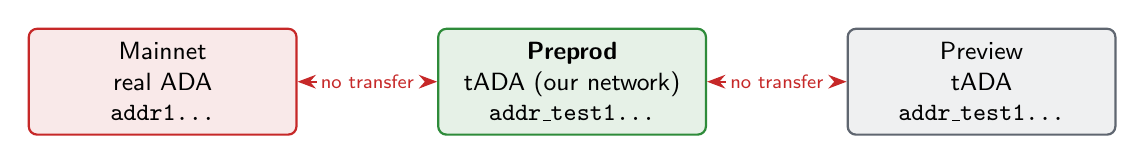
\begin{tikzpicture}
  \node[bad,minimum width=3.4cm] (m) at (0,0) {Mainnet\\real ADA\\\texttt{addr1...}};
  \node[good,minimum width=3.4cm] (p) at (5.2,0) {\textbf{Preprod}\\tADA (our network)\\\texttt{addr\_test1...}};
  \node[service,minimum width=3.4cm] (v) at (10.4,0) {Preview\\tADA\\\texttt{addr\_test1...}};
  \draw[<->,thick,draw=cRed,dashed] (m) -- node[lbl,text=cRed]{no transfer} (p);
  \draw[<->,thick,draw=cRed,dashed] (p) -- node[lbl,text=cRed]{no transfer} (v);
\end{tikzpicture}
\caption{Three separate networks. Preprod and preview addresses look alike, so always check the network setting in your tools.}
\end{figure}

\begin{warningbox}{Sokosumi MCP defaults to mainnet}
The Masumi runbook says: ``Confirm Preprod; mainnet default'' for the Sokosumi MCP server. Also use the \code{--preprod} flag in the Sokosumi CLI. In code, the network string in the x402 template is \code{cardano:preprod}.
\end{warningbox}

\section{Getting test ADA}

\subsection{The Cardano faucet}
The official \term{faucet} (documented under docs.cardano.org, ``Cardano testnets'') gives free tADA to a testnet address. The limits per claim are not stated in our notes.

\subsection{The Masumi dispenser}
The \term{Masumi dispenser} (dispenser.masumi.network) hands out test ADA and test USDM for the Masumi path. Facts from the runbooks:
\begin{itemize}
  \item it needs a \textbf{verification code from the Masumi registration email};
  \item it offers an optional separate \textbf{5 ADA collateral} claim;
  \item you must confirm it is on \textbf{preprod};
  \item funding of the Masumi seller wallet may take about 15--30 minutes to show up;
  \item per-claim amounts and limits are not documented: ask the mentors (open question).
\end{itemize}

\begin{figure}[h]
\centering
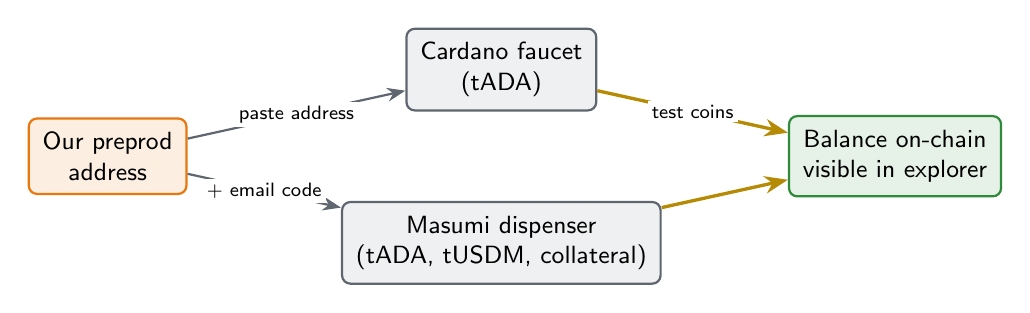
\begin{tikzpicture}
  \node[human] (w) at (0,0) {Our preprod\\address};
  \node[service] (f) at (5,1.1) {Cardano faucet\\(tADA)};
  \node[service] (d) at (5,-1.1) {Masumi dispenser\\(tADA, tUSDM, collateral)};
  \node[good] (b) at (10,0) {Balance on-chain\\visible in explorer};
  \draw[flow] (w) -- node[lbl]{paste address} (f);
  \draw[flow] (w) -- node[lbl]{+ email code} (d);
  \draw[pay] (f) -- node[lbl]{test coins} (b);
  \draw[pay] (d) -- (b);
\end{tikzpicture}
\caption{Two sources of free test funds. Both send coins to our address; we then see them in the explorer.}
\end{figure}

\section{Blockfrost: reading and submitting without running a node}

To talk to Cardano you normally need a full \term{node}: a program that downloads the whole chain (many gigabytes) and stays in sync. That is far too heavy for a hackathon laptop.

\term{Blockfrost} is a hosted API service: you send simple HTTP requests (with an API key, called a \emph{project ID}) and Blockfrost answers with chain data, or submits your signed transaction for you. Free accounts exist; creating one is a human step on blockfrost.io, and one project is tied to one network (we need a \textbf{preprod} project).

\begin{figure}[h]
\centering
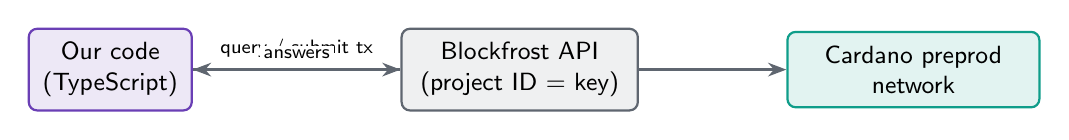
\begin{tikzpicture}
  \node[agent] (app) at (0,0) {Our code\\(TypeScript)};
  \node[service,minimum width=3cm] (bf) at (5.2,0) {Blockfrost API\\(project ID = key)};
  \node[chain,minimum width=3.2cm] (cn) at (10.2,0) {Cardano preprod\\network};
  \draw[flow] (app) -- node[lbl,above=2pt]{query / submit tx} (bf);
  \draw[flow,dashed] (bf) -- node[lbl,above=2pt]{answers} (app);
  \draw[flow] (bf) -- (cn);
\end{tikzpicture}
\caption{With Blockfrost we do not run a node: it relays reads and transaction submissions.}
\end{figure}

What we use it for: finding UTXOs of a wallet, building and submitting a transaction, checking whether a payment is confirmed. Notes from the runbooks:
\begin{itemize}
  \item the x402 template needs \code{BLOCKFROST\_PROJECT\_ID}; Masumi uses \code{BLOCKFROST\_API\_KEY\_PREPROD};
  \item the facilitator's \code{/verify} and \code{/settle} calls use Blockfrost quota;
  \item \textbf{a Blockfrost key in browser code is visible to everyone}, so keep it on the server;
  \item never commit the key to Git.
\end{itemize}

\section{Cardanoscan: reading a transaction}

\term{Cardanoscan} is a block explorer for Cardano. The preprod site is \code{preprod.cardanoscan.io}. A transaction page is reached with
\begin{center}
\code{https://preprod.cardanoscan.io/transaction/<tx hash>}
\end{center}
and an address page (inferred from the same host) with
\begin{center}
\code{https://preprod.cardanoscan.io/address/<address>}
\end{center}
The Masumi runbook asks us to paste the receipt's \code{txHash} into Cardanoscan, inspect the confirmed seller output, and save the resulting URL as evidence.

\begin{figure}[h]
\centering
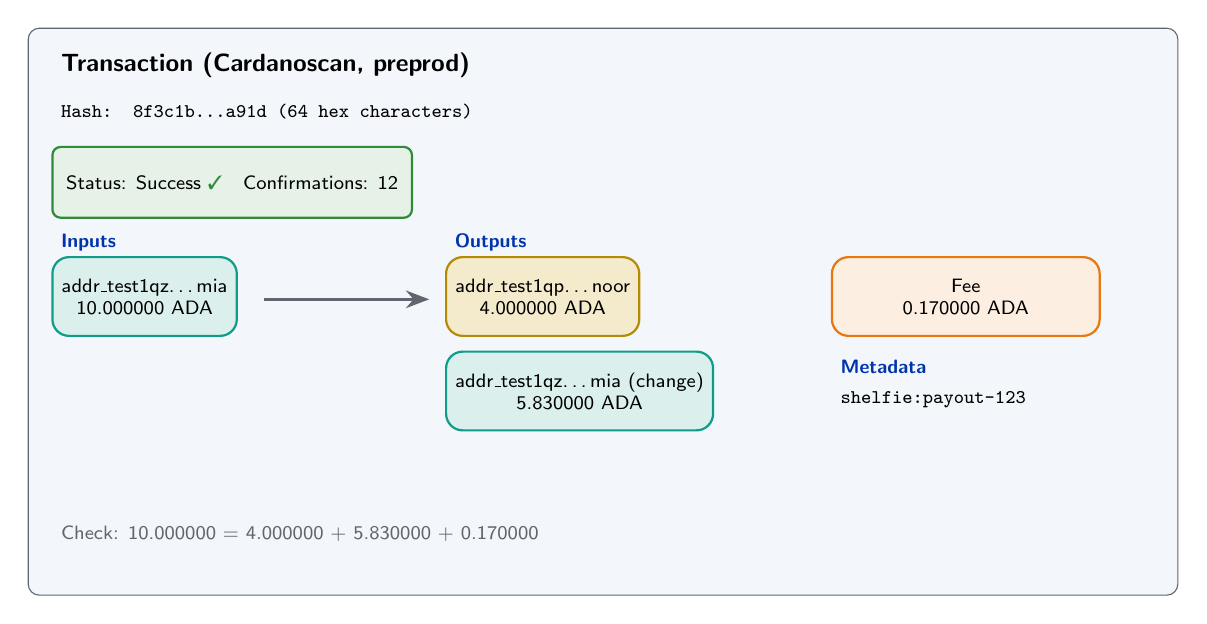
\begin{tikzpicture}
  \node[draw=cGrey,rounded corners=4pt,fill=cLight,minimum width=14.6cm,minimum height=7.2cm,anchor=north west] (page) at (0,0) {};
  \node[font=\sffamily\bfseries\small,anchor=north west] at (0.3,-0.2) {Transaction (Cardanoscan, preprod)};
  \node[font=\ttfamily\scriptsize,anchor=north west] at (0.3,-0.85) {Hash: 8f3c1b\ldots a91d  (64 hex characters)};
  \node[good,anchor=north west,font=\sffamily\scriptsize] at (0.3,-1.5) {Status: Success \yes\quad Confirmations: 12};
  % inputs
  \node[font=\sffamily\bfseries\scriptsize,anchor=north west,cBlue] at (0.3,-2.5) {Inputs};
  \node[utxo,anchor=north west] at (0.3,-2.9) {addr\_test1qz\ldots mia\\10.000000 ADA};
  % arrow
  \draw[->,very thick,draw=cGrey] (3.0,-3.45) -- (5.1,-3.45);
  % outputs
  \node[font=\sffamily\bfseries\scriptsize,anchor=north west,cBlue] at (5.3,-2.5) {Outputs};
  \node[utxo,anchor=north west,fill=cGold!20,draw=cGold!90!black] at (5.3,-2.9) {addr\_test1qp\ldots noor\\4.000000 ADA};
  \node[utxo,anchor=north west] at (5.3,-4.1) {addr\_test1qz\ldots mia (change)\\5.830000 ADA};
  \node[utxo,anchor=north west,fill=cOrange!12,draw=cOrange,minimum width=3.4cm] at (10.2,-2.9) {Fee\\0.170000 ADA};
  \node[font=\sffamily\bfseries\scriptsize,anchor=north west,cBlue] at (10.2,-4.1) {Metadata};
  \node[font=\ttfamily\scriptsize,anchor=north west] at (10.2,-4.5) {shelfie:payout-123};
  \node[font=\sffamily\scriptsize,anchor=north west,cGrey] at (0.3,-6.2) {Check: 10.000000 = 4.000000 + 5.830000 + 0.170000};
\end{tikzpicture}
\caption{A mock-up (not a real screenshot) of what a Cardanoscan transaction page shows. All values are invented.}
\end{figure}

\subsection{How to read it, field by field}
\begin{enumerate}
  \item \textbf{Hash:} the transaction's ID. Copy it to share or to search.
  \item \textbf{Status / confirmations:} ``Success'' and a growing confirmation count tell you the transaction is in the chain and how deep. Wait for several before treating a payment as final.
  \item \textbf{Inputs:} the UTXOs that were consumed and who owned them.
  \item \textbf{Outputs:} the new UTXOs: look for the \emph{recipient's address} and the amount. The other output is usually the change going back to the sender.
  \item \textbf{Fee:} what the network took.
  \item \textbf{Metadata:} optional tags such as our payout tag.
  \item Check the arithmetic: inputs $=$ outputs $+$ fee.
\end{enumerate}

\begin{warningbox}{Pending is not failed}
After an HTTP~402 or a dropped connection, a payment may still settle (runbook). Look at the buyer address on Cardanoscan before retrying, so that you do not pay twice.
\end{warningbox}

\begin{shelfiebox}{Receipts for judges}
For every payout and verifier fee, the Shelfie ledger stores the tx hash and a Cardanoscan URL, so each statement in our demo (``worker paid'') can be verified by clicking a link.
\end{shelfiebox}

\section{Wallet setup for the team}

Each teammate who sends or receives funds needs a Cardano wallet on preprod.

\begin{enumerate}
  \item \textbf{Generate a wallet.} The x402 template has a command (\code{npm run wallet}) that prints a fresh 24-word \textbf{mnemonic} and an \textbf{address} once. Copy them at once; they are shown only one time.
  \item \textbf{Store the mnemonic safely.} Put it in a private \code{.env} (listed in \code{.gitignore}), never in chat or Git. Use throwaway wallets only (Chapter~1).
  \item \textbf{Note the address.} It starts with \code{addr\_test1...} on preprod.
  \item \textbf{Fund it} from the faucet or the Masumi dispenser. Roughly 10~tADA covers many 2-tADA calls plus about 0.17 ADA fee each; the Masumi seller wallet needs about 20 tADA for registration (runbook).
  \item \textbf{Wait 1--2 minutes}, then check the address on Cardanoscan.
\end{enumerate}

Browser wallets (CIP-30 wallets that sign in a web page) are only needed for the demo UIs in the templates; our headless backend uses the mnemonic-based signer.

\begin{warningbox}{Two kinds of mnemonic prints}
The Masumi Payment Service seed command also prints mnemonics. The runbook says: operator only, no recording or screen sharing.
\end{warningbox}

\section{Cardano in our project}

Here is the map of what the team actually touches, and where.

\subsection{Concepts at a glance}
\begin{table}[h]
\centering
\small
\begin{tabularx}{\textwidth}{@{}p{3.6cm}X@{}}
\toprule
\textbf{Item} & \textbf{How Shelfie uses it}\\
\midrule
Network: \textbf{preprod} & every wallet, payment and explorer link; no mainnet anywhere\\
\textbf{tADA payouts} & verifier fee (default 1 tADA per check) and worker payouts, as plain transfers\\
\textbf{Blockfrost key} & one free preprod project; used by the x402 SDK, the facilitator fallback, and the Masumi Payment Service\\
\textbf{Cardanoscan links} & saved with each payout/fee as proof; shown on the worker page and in the pitch\\
\textbf{Metadata tag} & \code{shelfie:<payoutId>} on payouts, for crash-safe reconciliation\\
\textbf{Escrow} & Masumi's contract holds the brand's fee until the result is delivered; we do not write a validator\\
\textbf{Native tokens} & optional: tUSDM exists in the Masumi quote path, but our own prices are tADA\\
\textbf{Mnemonics} & stored only in private \code{.env} files; never in Git, chat or screen shares\\
\bottomrule
\end{tabularx}
\caption{Cardano concepts and their role in Shelfie.}
\end{table}

\subsection{The four wallets}
The design names wallets by purpose. Keeping them separate avoids UTXO contention and makes money flows easy to read.

\begin{table}[h]
\centering
\small
\begin{tabularx}{\textwidth}{@{}p{2.1cm}p{4.5cm}X@{}}
\toprule
\textbf{Wallet} & \textbf{Role} & \textbf{Explanation}\\
\midrule
\code{W-SELL} & verifier income & receives the x402 fee each time the engine buys a photo check from the verifier\\
\code{W-VBUY} & verifier buyer & the engine pays the verifier from here; one payment at a time (serial queue)\\
\code{W-PAY} & worker payouts & the engine pays workers from here after a photo passes; plain transfer, idempotent queue\\
\code{W-MPS} & Masumi seller wallet & used by the Masumi Payment Service (the seller side of the escrow); needs tADA and optional 5 ADA collateral\\
\bottomrule
\end{tabularx}
\caption{The named wallets from the design.}
\end{table}

Workers use their own preprod addresses (we do not hold their keys).

\begin{figure}[h]
\centering
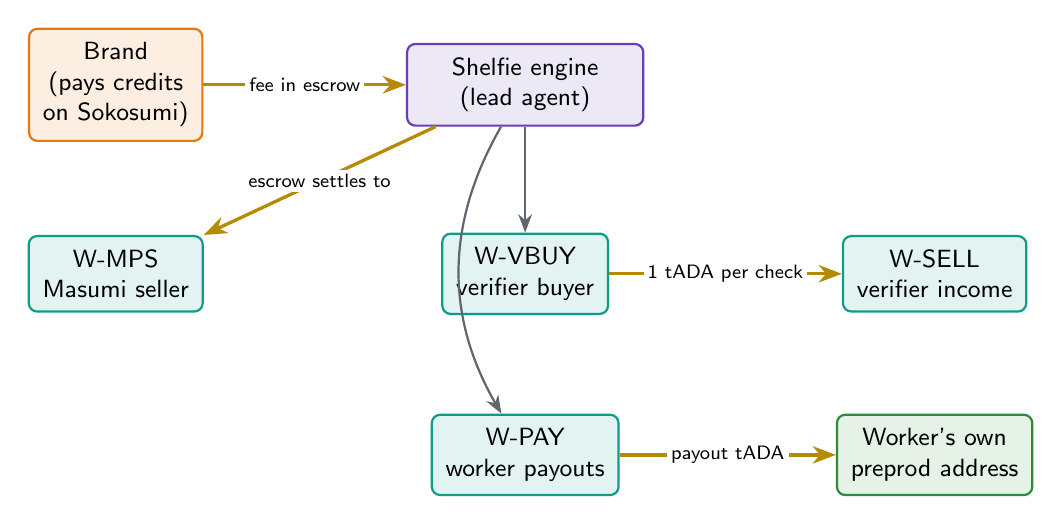
\begin{tikzpicture}
  \node[human] (brand) at (0,2.4) {Brand\\(pays credits\\on Sokosumi)};
  \node[agent,minimum width=3cm] (eng) at (5.2,2.4) {Shelfie engine\\(lead agent)};
  \node[chain] (wm) at (0,0) {W-MPS\\Masumi seller};
  \node[chain] (wv) at (5.2,0) {W-VBUY\\verifier buyer};
  \node[chain] (ws) at (10.4,0) {W-SELL\\verifier income};
  \node[chain] (wp) at (5.2,-2.3) {W-PAY\\worker payouts};
  \node[good] (wk) at (10.4,-2.3) {Worker's own\\preprod address};
  \draw[pay] (brand) -- node[lbl]{fee in escrow} (eng);
  \draw[pay] (eng) -- node[lbl]{escrow settles to} (wm.north east);
  \draw[pay] (wv) -- node[lbl]{1 tADA per check} (ws);
  \draw[pay] (wp) -- node[lbl]{payout tADA} (wk);
  \draw[flow] (eng) -- (wv);
  \draw[flow,bend right=30] (eng) to (wp);
\end{tikzpicture}
\caption{Simplified view of money flows between the named wallets. Blue/gold arrows are payments. The exact flow is explained in the architecture chapters.}
\end{figure}

\subsection{What stays unverified}
\begin{itemize}
  \item Whether the x402 template's SDK can send plain transfers with metadata (verify Friday, Task B, first 90 minutes). Fallbacks: Lucid or Mesh isolated behind a payout adapter; or manual payout flagged in the demo.
  \item Whether the hosted facilitator accepts a 1-tADA price (else 2 tADA).
  \item Faucet and dispenser per-claim limits.
  \item Which explorer judges prefer (Cexplorer preprod URL form not confirmed).
\end{itemize}

\begin{keypoints}
\begin{itemize}
  \item \textbf{ADA} is the coin; \textbf{1 ADA = 1{,}000{,}000 lovelace}. On the test network the coin is \textbf{tADA}.
  \item Cardano uses \textbf{Ouroboros} (Proof of Stake); holders may \textbf{delegate} to stake pools; irrelevant for the hackathon.
  \item \textbf{eUTXO:} the ledger holds unspent outputs; a transaction consumes inputs and creates outputs; inputs $=$ outputs $+$ fee.
  \item A \textbf{change output} sends the rest back to the sender; one wallet cannot make two parallel payments reliably, so we use separate wallets and serial queues.
  \item A \textbf{validator} decides whether a locked UTXO may be spent, using the \textbf{datum} (state) and the \textbf{redeemer} (action); languages: Plutus, Aiken.
  \item \textbf{Native tokens} need no smart contract; tUSDM has two incompatible versions, so we price in tADA.
  \item Fees are about 0.17 ADA; every output needs about 1 ADA \textbf{min-ADA}; \textbf{metadata} lets us tag payouts.
  \item We use \textbf{preprod}; test funds come from the faucet or the Masumi dispenser.
  \item \textbf{Blockfrost} lets us read and submit without a node; \textbf{Cardanoscan} shows the receipt (hash, inputs, outputs, fee, confirmations).
  \item Team wallets: \code{W-SELL}, \code{W-VBUY}, \code{W-PAY}, \code{W-MPS}; mnemonics stay in private \code{.env} files.
\end{itemize}
\end{keypoints}

\begin{quizbox}
\begin{enumerate}
  \item How many lovelace is 0.17 ADA? How many ADA is 3{,}500{,}000 lovelace?
  \item Mia owns UTXOs of 8 ADA and 3 ADA. She pays Noor 5 ADA with a fee of 0.2 ADA. Which input does the wallet probably pick, and what is the change output?
  \item In an escrow, what is the datum and what is the redeemer?
  \item Why can't a Shelfie payout of 0.3 tADA be sent?
  \item What does Blockfrost replace, and why must its key not be placed in browser code?
  \item Name the four wallets in our design and one purpose each.
\end{enumerate}
{\footnotesize\color{cGrey}\textbf{Answers.} (1) 170{,}000 lovelace; 3.5 ADA. (2) The 8-ADA UTXO; change $=8-5-0.2=2.8$ ADA (the 3-ADA UTXO stays untouched). (3) The datum is the stored agreement (buyer, seller, deadline); the redeemer is the spender's action (Release or Refund). (4) It is below the minimum ADA of an output (about 1 ADA). (5) Running your own full node; browser code is visible to everybody, so the key could be stolen. (6) W-SELL receives verifier fees, W-VBUY pays the verifier, W-PAY pays workers, W-MPS is the Masumi seller wallet.}
\end{quizbox}


\part{Payments and agents}
\chapter{HTTP 402 and x402}

\section*{Why this matters for us}
Shelfie sells exactly one thing to other software: a \emph{verification} of a shelf photo, for 1~tADA per check. The way we sell it is x402, the Cardano track's ``fastest path to a first payment''. Our engine (a program) pays our verifier (another program) over plain HTTP, with no accounts, no API keys and no invoices, and every payment leaves a transaction hash that judges can open on Cardanoscan. To understand how that works you need three layers: (1) what HTTP is, (2) what the unused status code \code{402 Payment Required} was meant for, and (3) how the x402 protocol finally gives it a meaning. This chapter builds those layers from zero and ends with the exact numbers we plan to use.

\section{HTTP from zero}
\subsection{Client, server, request, response}
The web works as a conversation between two programs. The \term{client} asks (your browser, a phone app, a script, an AI agent). The \term{server} answers (a program running on some computer, listening at an address such as \code{shelfie.example}). Each question is called a \term{request} and each answer a \term{response}. \term{HTTP} (HyperText Transfer Protocol) is the agreed format of these messages, so that any client can talk to any server.

\begin{center}
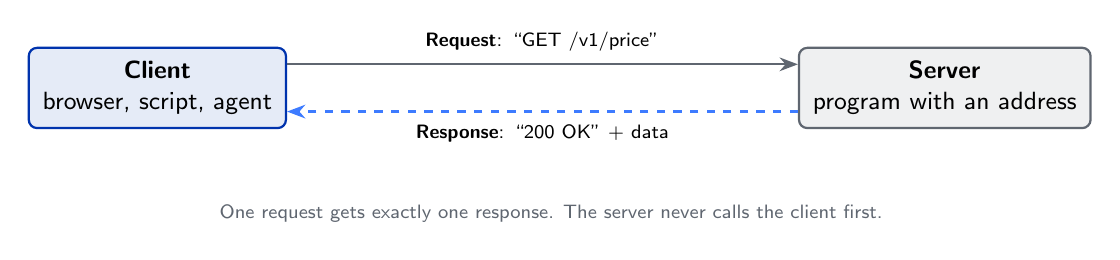
\begin{tikzpicture}[x=1cm,y=1cm]
  \node[actor,minimum width=3.2cm] (c) at (0,0) {\textbf{Client}\\browser, script, agent};
  \node[service,minimum width=3.2cm] (s) at (10,0) {\textbf{Server}\\program with an address};
  \draw[flow] ([yshift=3mm]c.east) -- ([yshift=3mm]s.west) node[lbl,above=1mm,fill=none] {\textbf{Request}: ``GET /v1/price''};
  \draw[data] ([yshift=-3mm]s.west) -- ([yshift=-3mm]c.east) node[lbl,below=1mm,fill=none] {\textbf{Response}: ``200 OK'' + data};
  \node[font=\sffamily\scriptsize,text=cGrey] at (5,-1.6) {One request gets exactly one response. The server never calls the client first.};
\end{tikzpicture}
\end{center}

\begin{analogybox}{a restaurant}
The client is a guest, the server is the kitchen, the request is the order slip and the response is the plate. The guest uses a fixed menu format (HTTP), so every kitchen understands every guest. If the kitchen needs a deposit before cooking, it should say so on the slip it hands back. That missing ``deposit'' answer is what HTTP~402 was reserved for.
\end{analogybox}

\subsection{Anatomy of a message}
A request has four parts and a response has three:
\begin{itemize}
  \item \term{Method}: what the client wants to do (\code{GET} = read, \code{POST} = send data to be processed).
  \item \term{URL / path}: which resource (\code{/v1/verify}).
  \item \term{Headers}: small labelled extra facts, one per line (\code{Content-Type: application/json}). x402 lives entirely in headers.
  \item \term{Body}: the payload (for us: JSON containing a photo).
  \item In the response, the \term{status code} is a three-digit number plus a short text that says how it went.
\end{itemize}

\begin{center}
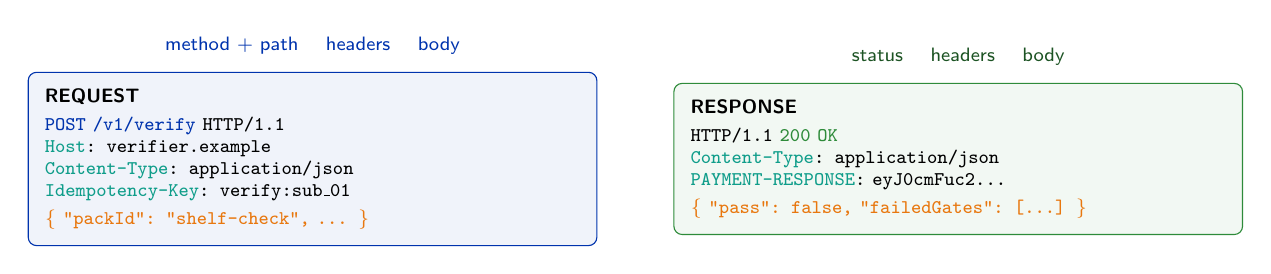
\begin{tikzpicture}[x=1cm,y=1cm,every node/.style={font=\ttfamily\scriptsize}]
  \node[draw=cBlue,fill=cBlue!6,rounded corners=3pt,align=left,inner sep=6pt,text width=6.8cm] (rq) at (0,0)
   {\textbf{\sffamily REQUEST}\\[2pt]
    \textcolor{cBlue}{POST /v1/verify} HTTP/1.1\\
    \textcolor{cTeal}{Host}: verifier.example\\
    \textcolor{cTeal}{Content-Type}: application/json\\
    \textcolor{cTeal}{Idempotency-Key}: verify:sub\_01\\[2pt]
    \textcolor{cOrange}{\{ "packId": "shelf-check", ... \}}};
  \node[draw=cGreen,fill=cGreen!6,rounded corners=3pt,align=left,inner sep=6pt,text width=6.8cm] (rs) at (8.2,0)
   {\textbf{\sffamily RESPONSE}\\[2pt]
    HTTP/1.1 \textcolor{cGreen}{200 OK}\\
    \textcolor{cTeal}{Content-Type}: application/json\\
    \textcolor{cTeal}{PAYMENT-RESPONSE}: eyJ0cmFuc2...\\[2pt]
    \textcolor{cOrange}{\{ "pass": false, "failedGates": [...] \}}};
  \node[font=\sffamily\scriptsize,text=cBlue,above=1mm of rq] {method + path \quad headers \quad body};
  \node[font=\sffamily\scriptsize,text=cGreen!60!black,above=1mm of rs] {status \quad headers \quad body};
\end{tikzpicture}
\end{center}

\subsection{The status codes you must know}
The first digit is the family: 2xx = success, 3xx = look elsewhere, 4xx = the \emph{client} did something wrong or is missing something, 5xx = the \emph{server} failed.

\begin{center}
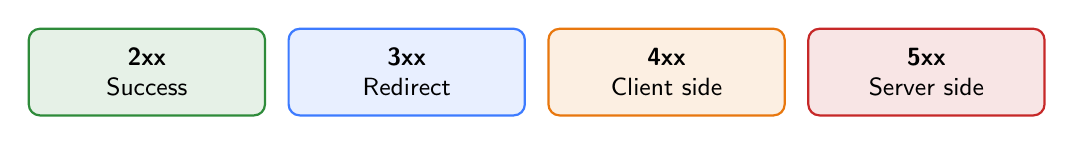
\begin{tikzpicture}[x=1cm,y=1cm]
  \foreach \x/\t/\c/\d in {0/2xx/cGreen/Success,3.3/3xx/cSky/Redirect,6.6/4xx/cOrange/Client side,9.9/5xx/cRed/Server side}{
    \node[draw=\c,fill=\c!12,thick,rounded corners=4pt,minimum width=3cm,minimum height=1.1cm,align=center,font=\sffamily\small] at (\x+1.5,0) {\textbf{\t}\\\d};}
\end{tikzpicture}
\end{center}

\begin{center}
\small
\begin{tabularx}{\textwidth}{@{}l l X@{}}
\toprule
\textbf{Code} & \textbf{Name} & \textbf{Meaning in plain words}\\
\midrule
\code{200} & OK & It worked, here is what you asked for.\\
\code{301} & Moved Permanently & The thing now lives at another URL; go there.\\
\code{400} & Bad Request & Your request is malformed (broken JSON, missing field).\\
\code{401} & Unauthorized & ``Who are you?'' Log in or send credentials.\\
\code{403} & Forbidden & I know who you are, but you may not do this.\\
\code{404} & Not Found & There is nothing at this address.\\
\textcolor{cPurple}{\textbf{\code{402}}} & \textcolor{cPurple}{\textbf{Payment Required}} & \textcolor{cPurple}{\textbf{You must pay first.} Reserved since the 1990s, now used by x402.}\\
\code{500} & Internal Server Error & The server crashed or failed; not your fault.\\
\bottomrule
\end{tabularx}
\end{center}

\begin{examplebox}{reading Shelfie's own error codes}
In our verifier contract (\code{diseno/contracts.md}), errors before payment settles use \code{400 invalid\_request}, \code{413 image\_too\_large}, \code{422 image\_not\_decodable} and \code{503 vision\_unavailable}. Codes 413, 422 and 503 are standard HTTP codes that we simply reuse: ``payload too large'', ``cannot process this content'' and ``service temporarily unavailable''. The design goal is that these must \emph{not} charge the buyer.
\end{examplebox}

\section{The history of \texttt{402 Payment Required}}
When the HTTP status codes were designed in the 1990s, the authors expected money to move on the web soon. They set aside code \code{402} with the name ``Payment Required'' and the note ``reserved for future use''. The idea: a server could answer 402 to say ``this resource costs money''.

Then nothing happened. No standard defined \emph{how} to say the price, \emph{in which currency}, or \emph{how} to prove payment. Credit-card networks, PayPal and later Stripe built their own checkouts on top of web pages instead. For about thirty years \code{402} stayed an unused code: browsers show it like any 4xx error, and a few services misuse it informally (for example ``your subscription lapsed'').

\begin{center}
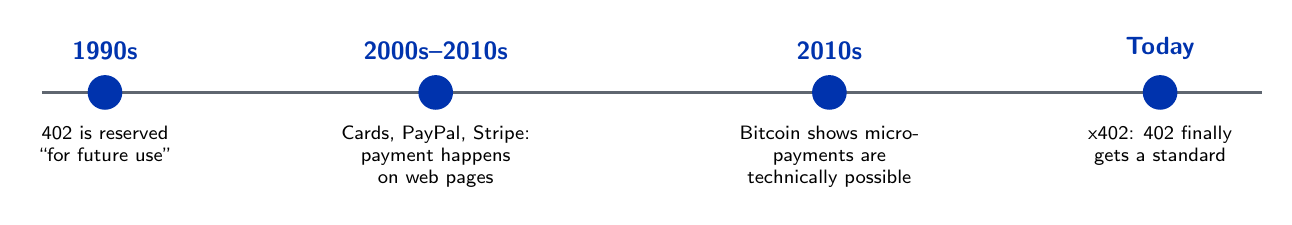
\begin{tikzpicture}[x=1cm,y=1cm]
  \draw[thick,draw=cGrey] (0,0) -- (15.5,0);
  \foreach \x/\t in {0.8/1990s,5/2000s--2010s,10/2010s,14.2/Today}{
    \fill[cBlue] (\x,0) circle (2.2mm);
    \node[font=\sffamily\small\bfseries,above=3mm,text=cBlue] at (\x,0) {\t};}
  \node[font=\sffamily\scriptsize,below=3mm,align=center] at (0.8,0) {402 is reserved\\``for future use''};
  \node[font=\sffamily\scriptsize,below=3mm,align=center] at (5,0) {Cards, PayPal, Stripe:\\payment happens\\on web pages};
  \node[font=\sffamily\scriptsize,below=3mm,align=center] at (10,0) {Bitcoin shows micro-\\payments are\\technically possible};
  \node[font=\sffamily\scriptsize,below=3mm,align=center] at (14.2,0) {x402: 402 finally\\gets a standard};
\end{tikzpicture}
\end{center}

\begin{conceptbox}{Why 402 is attractive again}
Three things changed. (1) Blockchains give a payment method that works without a bank, around the clock, in any amount. (2) Settlement takes seconds to a minute and costs cents or less, so tiny prices make sense. (3) The biggest new customers of the web are no longer humans with credit cards but \emph{software agents}, which cannot fill in a checkout form. x402 is the protocol that turns the dormant status code into a working payment handshake.
\end{conceptbox}

\section{Why paying per request matters for machines}
Think about how a program normally buys a service today. A human signs up, enters a credit card, receives an \term{API key} (a secret password string), and the program sends that key in every request. That works, but it has costs that grow when the buyer is an autonomous agent:
\begin{itemize}
  \item \textbf{Accounts and onboarding.} Someone must register, accept terms, and store the key. An agent that discovers a new service at 3~a.m.\ cannot do this alone.
  \item \textbf{Subscriptions.} A flat monthly fee is wasteful if you need 12 checks this week and none next week.
  \item \textbf{Minimum charges.} Card fees (often a fixed part of tens of cents plus a percentage) make a price of 1 cent or 10 cents impossible. These are \term{micropayments}.
  \item \textbf{Secrets management.} A leaked API key lets strangers spend your money.
\end{itemize}

x402 flips this. The \emph{request itself} carries the payment, one request at a time. The seller needs no list of customers and the buyer needs no account.

\begin{analogybox}{a vending machine versus a gym membership}
A gym membership means registration, a contract and a monthly debit whether you use it or not (subscription + API key). A vending machine lets anyone walk up, put coins in and receive exactly one item (pay per request). The machine does not know you and does not need to. x402 turns every API into a vending machine, and the ``coins'' are a signed blockchain payment.
\end{analogybox}

\section{The x402 protocol}
\subsection{Roles}
\begin{center}
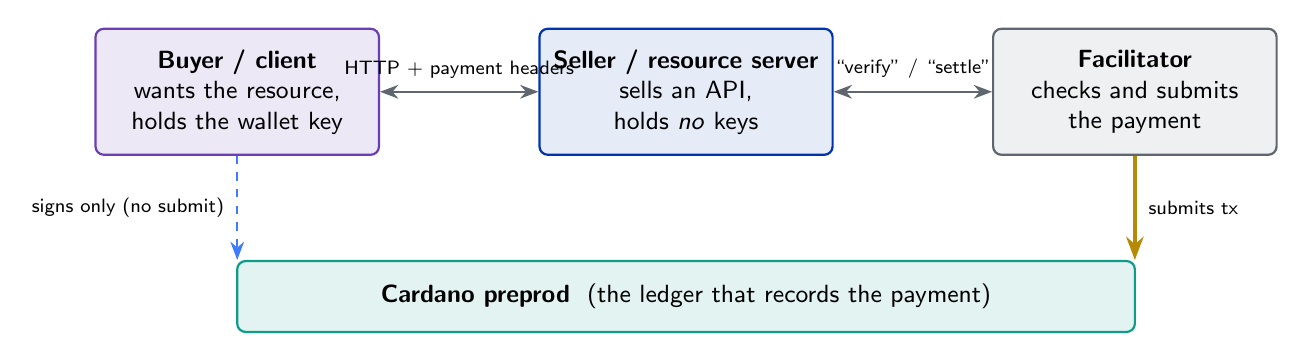
\begin{tikzpicture}[x=1cm,y=1cm]
  \node[agent,minimum width=3.6cm,minimum height=1.6cm] (b) at (0,0) {\textbf{Buyer / client}\\wants the resource,\\holds the wallet key};
  \node[actor,minimum width=3.6cm,minimum height=1.6cm] (s) at (5.7,0) {\textbf{Seller / resource server}\\sells an API,\\holds \emph{no} keys};
  \node[service,minimum width=3.6cm,minimum height=1.6cm] (f) at (11.4,0) {\textbf{Facilitator}\\checks and submits\\the payment};
  \node[chain,minimum width=11.4cm] (c) at (5.7,-2.6) {\textbf{Cardano preprod}\ \ (the ledger that records the payment)};
  \draw[flow,<->] (b) -- (s) node[lbl,midway,above=1mm,fill=none] {HTTP + payment headers};
  \draw[flow,<->] (s) -- (f) node[lbl,midway,above=1mm,fill=none] {``verify'' / ``settle''};
  \draw[pay] (f.south) -- (f.south |- c.north) node[lbl,midway,right=1mm,fill=none] {submits tx};
  \draw[data] (b.south) -- (b.south |- c.north) node[lbl,midway,left=1mm,fill=none] {signs only (no submit)};
\end{tikzpicture}
\end{center}

\begin{itemize}
  \item The \term{buyer} (client) is the party that wants something. It holds a wallet key and \emph{signs} the payment.
  \item The \term{seller} (resource server) owns the API. It only needs a receiving address, never a private key. This is why a seller cannot lose funds to a hack of its server.
  \item The \term{facilitator} is a helper service. It checks that a signed payment is valid (\term{verify}) and submits it to the blockchain (\term{settle}). It exists so the seller does not need blockchain code or a node connection. On Cardano the hosted preprod facilitator is \term{non-custodial}: it never holds the buyer's money or keys.
\end{itemize}

\subsection{The full flow}
The key trick is the \emph{two-step request}. The buyer first asks without paying, learns the price from a 402 answer, signs a payment, and asks again with the payment attached.

\begin{center}
\resizebox{\textwidth}{!}{%
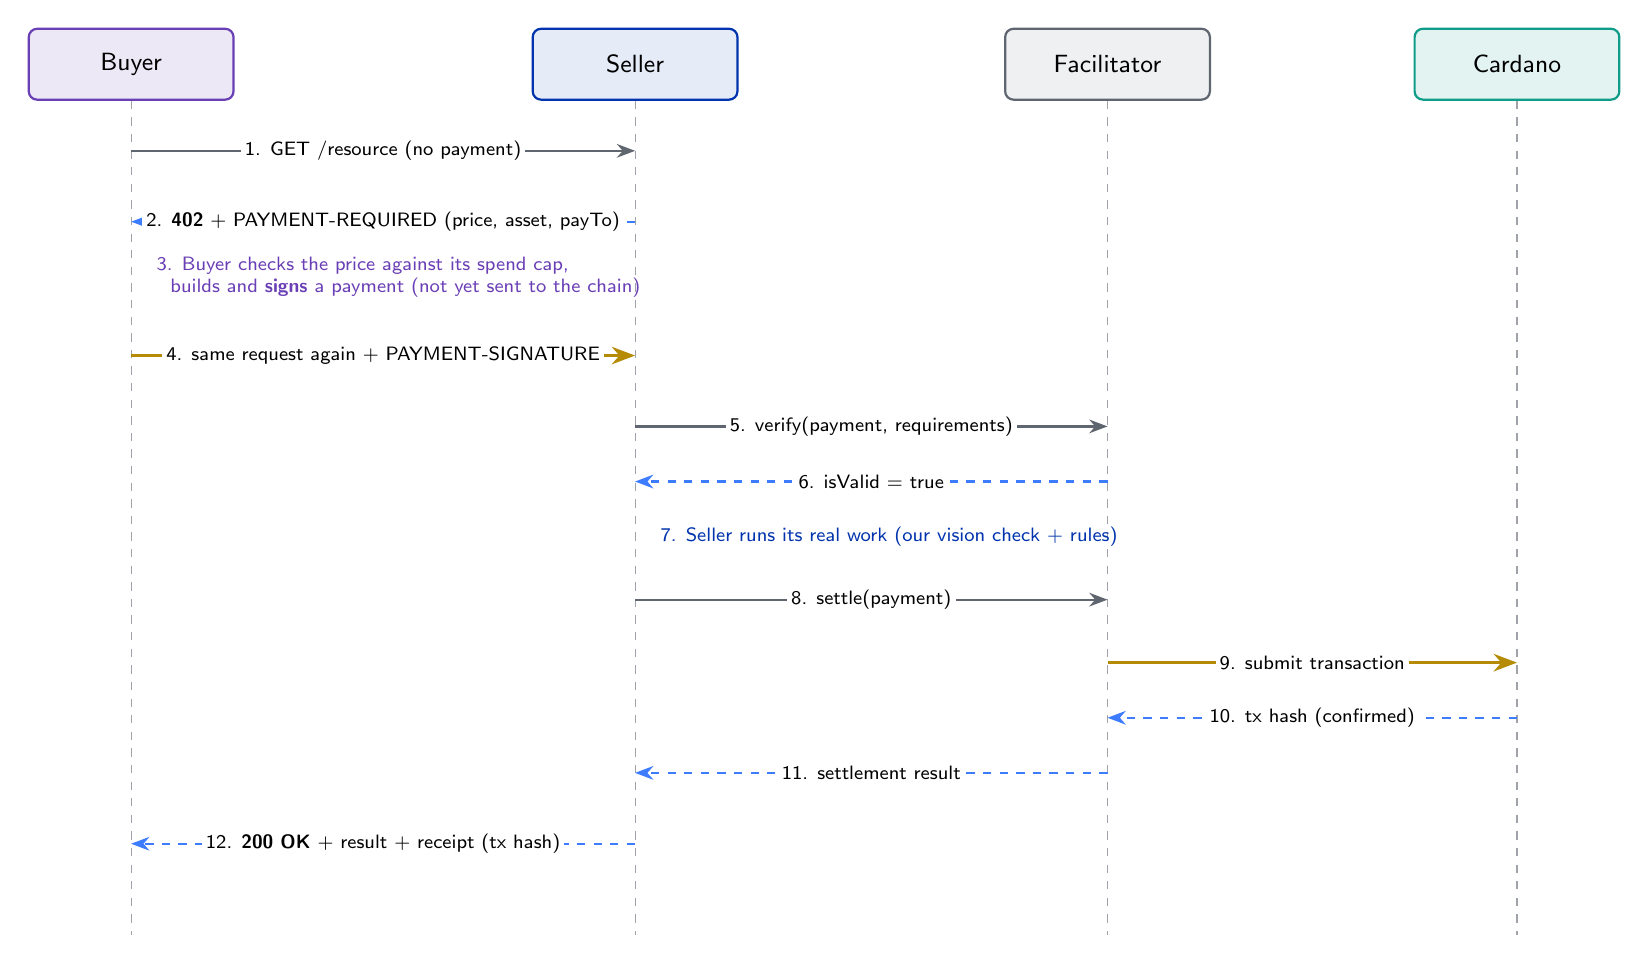
\begin{tikzpicture}[x=1cm,y=1cm,
   life/.style={dashed,draw=cGrey!60},
   msg/.style={->,thick,draw=cGrey},
   payl/.style={->,very thick,draw=cGold!90!black},
   ret/.style={->,thick,dashed,draw=cSky},
   n/.style={font=\sffamily\scriptsize,fill=white,inner sep=1.5pt,align=center}]
  \node[agent,minimum width=2.6cm] (B) at (0,0) {Buyer};
  \node[actor,minimum width=2.6cm] (S) at (6.4,0) {Seller};
  \node[service,minimum width=2.6cm] (F) at (12.4,0) {Facilitator};
  \node[chain,minimum width=2.6cm] (C) at (17.6,0) {Cardano};
  \foreach \p in {B,S,F,C} \draw[life] (\p.south) -- ++(0,-10.6);
  \draw[msg] (0,-1.1) -- (6.4,-1.1) node[n,midway] {1. GET /resource (no payment)};
  \draw[ret] (6.4,-2.0) -- (0,-2.0) node[n,midway] {2. \textbf{402} + PAYMENT-REQUIRED (price, asset, payTo)};
  \node[font=\sffamily\scriptsize,text=cPurple,align=left,anchor=west] at (0.2,-2.7) {3. Buyer checks the price against its spend cap,\\ \ \ builds and \textbf{signs} a payment (not yet sent to the chain)};
  \draw[payl] (0,-3.7) -- (6.4,-3.7) node[n,midway] {4. same request again + PAYMENT-SIGNATURE};
  \draw[msg] (6.4,-4.6) -- (12.4,-4.6) node[n,midway] {5. verify(payment, requirements)};
  \draw[ret] (12.4,-5.3) -- (6.4,-5.3) node[n,midway] {6. isValid = true};
  \node[font=\sffamily\scriptsize,text=cBlue,anchor=west] at (6.6,-6.0) {7. Seller runs its real work (our vision check + rules)};
  \draw[msg] (6.4,-6.8) -- (12.4,-6.8) node[n,midway] {8. settle(payment)};
  \draw[payl] (12.4,-7.6) -- (17.6,-7.6) node[n,midway] {9. submit transaction};
  \draw[ret] (17.6,-8.3) -- (12.4,-8.3) node[n,midway] {10. tx hash (confirmed)};
  \draw[ret] (12.4,-9.0) -- (6.4,-9.0) node[n,midway] {11. settlement result};
  \draw[ret] (6.4,-9.9) -- (0,-9.9) node[n,midway] {12. \textbf{200 OK} + result + receipt (tx hash)};
\end{tikzpicture}}
\end{center}

\begin{examplebox}{the same flow with numbers}
A buyer calls \code{POST /v1/verify}. Step 2 returns: ``price 1000000 lovelace, asset lovelace, network cardano:preprod, payTo addr\_test1\ldots''. The buyer's cap is 2000000 lovelace, so it accepts (1~tADA $\le$ 2~tADA). It signs a transaction moving 1~tADA to the seller's address and retries (steps 3--4). The facilitator confirms the signature and balance (steps 5--6). The seller does its work, the facilitator submits the transaction (step 9), and after 20--60~s the buyer receives the verdict plus the transaction hash (step 12). Network fee: about 0.17~ADA on top, paid by the buyer.
\end{examplebox}

\subsection{What is in the payment requirements}
The 402 answer carries a small structured document (header \code{PAYMENT-REQUIRED}) that tells the buyer everything it needs to decide and pay:

\begin{center}
\small
\begin{tabularx}{\textwidth}{@{}l l X@{}}
\toprule
\textbf{Field} & \textbf{Example} & \textbf{Meaning}\\
\midrule
\code{scheme} & \code{exact} & Pay exactly the stated amount (no ``up to'').\\
\code{network} & \code{cardano:preprod} & Which chain; here the practice network.\\
\code{price.amount} & \code{1000000} & The price in the asset's smallest unit.\\
\code{price.asset} & \code{lovelace} & What to pay with: ADA (in lovelace) or a token.\\
\code{payTo} & \code{addr\_test1\ldots} & The seller's receiving address.\\
\code{description} & ``One shelf-photo verification'' & Human-readable purpose.\\
\code{mimeType} & \code{application/json} & Type of the thing you will get back.\\
\bottomrule
\end{tabularx}
\end{center}

\noindent Remember: 1~ADA = 1\,000\,000 lovelace, and on the test network the coin is called \emph{tADA} (worthless test money from a faucet).

\subsection{The three headers}
\begin{center}
\small
\begin{tabularx}{\textwidth}{@{}l l X@{}}
\toprule
\textbf{Header} & \textbf{Direction} & \textbf{Content}\\
\midrule
\code{PAYMENT-REQUIRED} & seller $\rightarrow$ buyer (with 402) & The payment requirements above.\\
\code{PAYMENT-SIGNATURE} & buyer $\rightarrow$ seller (retry) & The signed payment, encoded as text.\\
\code{PAYMENT-RESPONSE} & seller $\rightarrow$ buyer (with 200) & The receipt: success flag and the transaction hash.\\
\bottomrule
\end{tabularx}
\end{center}

\subsection{Verify versus settle}
These two facilitator steps are easy to confuse and matter for correctness.
\begin{itemize}
  \item \term{Verify} is a \emph{check only}: ``Is this signature valid? Does the buyer have the funds? Does the payment match the requirements?'' Nothing is sent to the chain, nothing is spent. A failed check arrives as HTTP~200 with \code{isValid:false} and an \code{invalidReason}; do not mistake that 200 for ``paid''.
  \item \term{Settle} actually submits the transaction and waits for the chain to confirm it. Only now has money moved.
\end{itemize}
In the Cardano express template the seller's paid handler runs \emph{after verify and before settle}. This gives the seller a safe ``go/no-go'' point: it can refuse to do work for an invalid payment, and the buyer is charged only when settlement happens.

\begin{center}
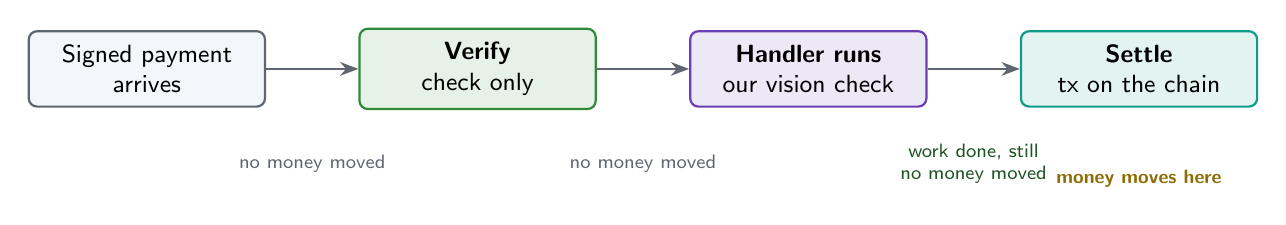
\begin{tikzpicture}[x=1cm,y=1cm]
  \node[box,fill=cLight,draw=cGrey,minimum width=3cm] (a) at (0,0) {Signed payment\\arrives};
  \node[good,minimum width=3cm] (v) at (4.2,0) {\textbf{Verify}\\check only};
  \node[agent,minimum width=3cm] (h) at (8.4,0) {\textbf{Handler runs}\\our vision check};
  \node[chain,minimum width=3cm] (s) at (12.6,0) {\textbf{Settle}\\tx on the chain};
  \draw[flow] (a)--(v); \draw[flow] (v)--(h); \draw[flow] (h)--(s);
  \node[font=\sffamily\scriptsize,text=cGrey,align=center] at (2.1,-1.2) {no money moved};
  \node[font=\sffamily\scriptsize,text=cGrey,align=center] at (6.3,-1.2) {no money moved};
  \node[font=\sffamily\scriptsize,text=cGreen!60!black,align=center] at (10.5,-1.2) {work done, still\\no money moved};
  \node[font=\sffamily\scriptsize,text=cGold!70!black,align=center] at (12.6,-1.4) {\textbf{money moves here}};
\end{tikzpicture}
\end{center}

\begin{warningbox}{the handler can run more than once}
Because retries happen (timeouts, dropped connections), the paid handler may be called again for the same payment. Our verifier therefore stores each verdict under an \code{Idempotency-Key} and, on a repeat, returns the cached answer without calling the vision model a second time.
\end{warningbox}


\subsection{What a 402 exchange looks like on the wire}
To make this concrete, here is the exchange in simplified form. The header values are really long encoded strings; they are shortened here with dots.
\begin{lstlisting}
--- first request (no payment) ---
POST /v1/verify HTTP/1.1
Idempotency-Key: verify:sub_01

--- first response ---
HTTP/1.1 402 Payment Required
PAYMENT-REQUIRED: eyJzY2hlbWUiOiJleGFjdCIs...   (price, asset, payTo, network)

--- second request (same call, now with payment) ---
POST /v1/verify HTTP/1.1
Idempotency-Key: verify:sub_01
PAYMENT-SIGNATURE: eyJwYXlsb2FkIjoi...          (signed payment)

--- second response ---
HTTP/1.1 200 OK
PAYMENT-RESPONSE: eyJzdWNjZXNzIjp0cnVl...       (receipt: transaction hash)
{ "pass": false, "failedGates": ["code_match"] }
\end{lstlisting}
The values are encoded (base64 text) so they fit safely in a header; the libraries encode and decode them for us. We never write this by hand.

\subsection{How an agent decides whether to pay}
A human reads a price and decides. An agent needs a rule. The buyer wrapper turns the human decision into a short, checkable procedure:
\begin{center}
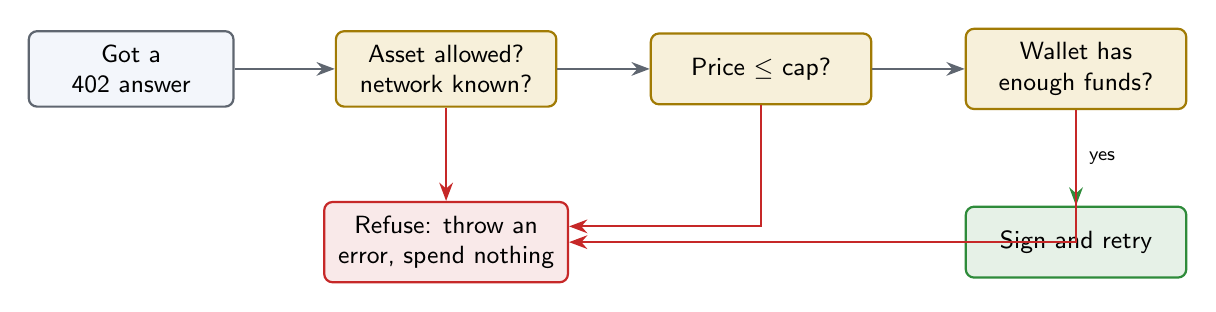
\begin{tikzpicture}[x=1cm,y=1cm,node distance=5mm]
  \node[box,fill=cLight,draw=cGrey,minimum width=2.6cm] (a) at (0,0) {Got a\\402 answer};
  \node[box,fill=cGold!15,draw=cGold!80!black,minimum width=2.8cm] (b) at (4,0) {Asset allowed?\\network known?};
  \node[box,fill=cGold!15,draw=cGold!80!black,minimum width=2.8cm] (c) at (8,0) {Price $\le$ cap?};
  \node[box,fill=cGold!15,draw=cGold!80!black,minimum width=2.8cm] (d) at (12,0) {Wallet has\\enough funds?};
  \node[good,minimum width=2.8cm] (ok) at (12,-2.2) {Sign and retry};
  \node[bad,minimum width=2.8cm] (no) at (4,-2.2) {Refuse: throw an\\error, spend nothing};
  \draw[flow] (a)--(b); \draw[flow] (b)--(c); \draw[flow] (c)--(d);
  \draw[flow,draw=cGreen] (d)--(ok) node[lbl,midway,right=1mm,fill=none] {yes};
  \draw[flow,draw=cRed] (b)--(no); \draw[flow,draw=cRed] (c) |- ([yshift=2mm]no.east); \draw[flow,draw=cRed] (d) |- (no.east);
\end{tikzpicture}
\end{center}
Every ``no'' ends in refusal rather than payment. This is exactly why the cap and the asset allow-list are not optional extras.

\begin{examplebox}{a hostile or buggy seller}
Suppose our verifier URL is mistyped and points to a stranger's server that answers 402 asking for 400~tADA. The wrapper compares 400\,000\,000 lovelace with the cap of 2\,000\,000, refuses, and the call fails with an error. Without a cap, one wrong string could empty the wallet. On the test network the loss would be only worthless tADA, but the habit has to be right before it ever touches mainnet money.
\end{examplebox}

\section{x402 on Cardano}
The Cardano Foundation provides ready-made parts so we do not implement any of the above by hand. All of these are from the team's runbook (\code{investigacion/cardano/x402-runbook.md}); nothing has been executed yet, so treat them as \emph{plan}, not as proven.

\begin{center}
\small
\begin{tabularx}{\textwidth}{@{}l X@{}}
\toprule
\textbf{Part} & \textbf{What it is / how we use it}\\
\midrule
\code{@x402/cardano} & The Cardano payment scheme (\code{exact}), with both a client signer and a server verifier. Pinned at version 2.26.0 together with \code{@x402/core}, \code{@x402/express}, \code{@x402/fetch}.\\
Hosted preprod facilitator & Public, non-custodial, needs no key. URL in the template's \code{.env.example}. The public x402.org facilitator does \emph{not} support Cardano. Fallback: run a local facilitator (\code{npm run facilitator}, about 100 lines, needs a Blockfrost key).\\
\code{x402-express} template & A small seller (Express server with payment middleware) plus a buyer script, both in TypeScript. Created with the \code{giget} command from the Cardano developer portal.\\
Headless buyer signer & \code{toClientCardanoSigner} signs from a 24-word \emph{mnemonic} stored in \code{.env}. No browser wallet is needed; that is what lets a program pay.\\
\code{npm run wallet} & Generates a fresh mnemonic and address (shown once).\\
\code{npm run demo} & Starts the seller, runs the buyer once, stops. First paid transaction in about 30--60 minutes including keys and faucet (our estimate).\\
Blockfrost & A free API service that lets our code read and submit to the preprod chain; needs a free project id.\\
\bottomrule
\end{tabularx}
\end{center}

\subsection{The buyer side: \texttt{fetchWithPayment}}
In the buyer, the normal \code{fetch} function is wrapped so that it understands 402. In shape (simplified from the template):
\begin{lstlisting}
const client = new x402Client().setSpendControls({
  allowedAssets: [{ network: "cardano:*", asset: "lovelace",
                    maxAmountPerPayment: "5000000" }] });   // cap
client.register("cardano:*", new ExactCardanoScheme(signer));
const fetchWithPayment = wrapFetchWithPayment(fetch, client);
const res = await fetchWithPayment(url, { method: "GET" });
\end{lstlisting}
The \term{per-payment cap} (\code{maxAmountPerPayment}) is a safety fuse: if a seller suddenly asks for 500~tADA the wrapper refuses to sign. Lovelace is rejected by default (it is not pegged to a currency), so the allow-list entry is mandatory. Our plan sets the cap to 2\,000\,000 lovelace for a 1\,000\,000 price.

\subsection{The seller side}
The seller registers one route with its price and receiving address; the middleware does the rest. The seller holds no keys, only \code{SELLER\_ADDRESS}.
\begin{lstlisting}
app.use(paymentMiddleware({
  "POST /v1/verify": { accepts: [{ scheme: "exact",
      network: "cardano:preprod",
      price: { amount: "1000000", asset: "lovelace" },
      payTo }], description: "One shelf-photo verification",
    mimeType: "application/json" } }, resourceServer));
\end{lstlisting}
(The template's example route is \code{GET /api/message}; ours is the contract in \code{diseno/contracts.md}.)

\begin{warningbox}{limits to remember}
Lovelace routes need a price of at least 1~tADA (the chain's minimum output size), so 1~tADA is our floor; if the facilitator rejects it we move to 2~tADA (\emph{verify Friday}). One wallet cannot pay twice at the same moment, because the first coin it spends doubles as a unique nonce; we use one serial queue per wallet. Python has no supported Cardano x402 client, so the paying code stays in TypeScript. Two different test-USDM tokens exist, which is why we price in lovelace.
\end{warningbox}

\section{Worked example: the Shelfie verifier}
Shelfie's engine receives a photo from a human worker. It must decide whether the photo proves the product is on the shelf. The decision is made by a separate \emph{verifier service}, and we deliberately sell it through x402 so ``agent pays agent'' is visible on-chain.

\begin{center}
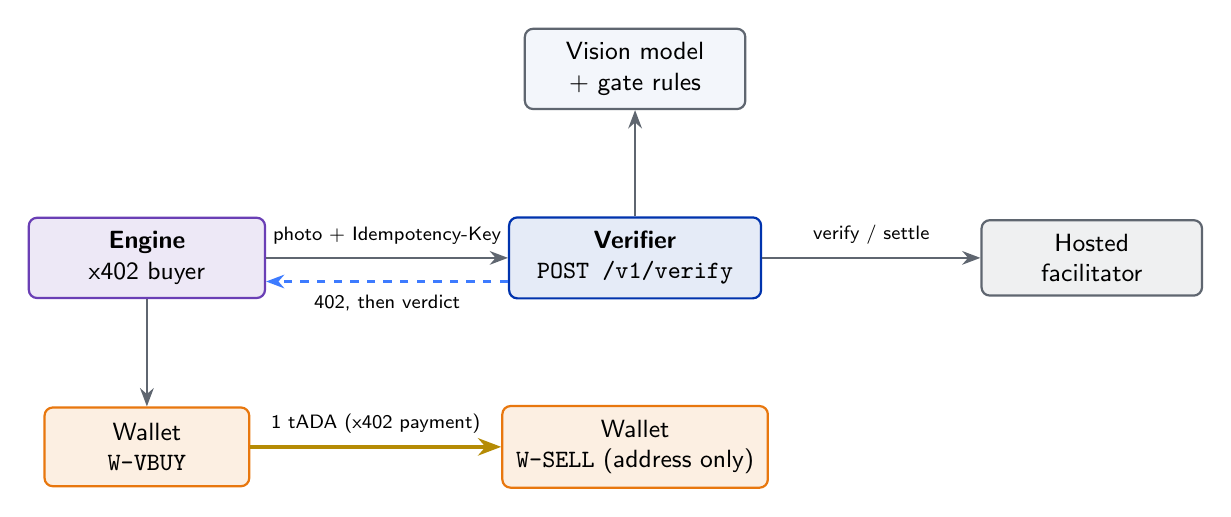
\begin{tikzpicture}[x=1cm,y=1cm]
  \node[agent,minimum width=3.0cm] (e) at (0,0) {\textbf{Engine}\\x402 buyer};
  \node[human,minimum width=2.6cm,minimum height=1cm] (wv) at (0,-2.4) {Wallet\\\code{W-VBUY}};
  \node[actor,minimum width=3.2cm] (v) at (6.2,0) {\textbf{Verifier}\\\code{POST /v1/verify}};
  \node[human,minimum width=2.6cm,minimum height=1cm] (ws) at (6.2,-2.4) {Wallet\\\code{W-SELL} (address only)};
  \node[service,minimum width=2.8cm] (f) at (12,0) {Hosted\\facilitator};
  \node[box,fill=cLight,draw=cGrey,minimum width=2.8cm] (vm) at (6.2,2.4) {Vision model\\+ gate rules};
  \draw[flow] (e) -- (v) node[lbl,midway,above=1mm,fill=none] {photo + Idempotency-Key};
  \draw[data] ([yshift=-3mm]v.west) -- ([yshift=-3mm]e.east) node[lbl,midway,below=1mm,fill=none] {402, then verdict};
  \draw[flow] (v) -- (f) node[lbl,midway,above=1mm,fill=none] {verify / settle};
  \draw[flow] (v) -- (vm);
  \draw[pay] (wv) -- (ws) node[lbl,midway,above=1mm,fill=none] {1 tADA (x402 payment)};
  \draw[flow] (e) -- (wv);
\end{tikzpicture}
\end{center}

\subsection{Endpoint, price and environment}
\begin{center}
\small
\begin{tabularx}{\textwidth}{@{}l X@{}}
\toprule
\textbf{Item} & \textbf{Planned value (from \code{diseno/contracts.md})}\\
\midrule
Paid endpoint & \code{POST /v1/verify}, protected by x402 seller middleware\\
Price & 1~tADA = \code{VERIFY\_PRICE\_LOVELACE=1000000}, \emph{per check, whether the photo passes or fails}\\
Asset / network & lovelace, \code{cardano:preprod}\\
Pay-to & address of wallet \code{W-SELL}, from env \code{SELLER\_ADDRESS}\\
Buyer cap & \code{VERIFY\_MAX\_PRICE\_LOVELACE=2000000} (2~tADA per payment)\\
Required header & \code{Idempotency-Key: verify:<submissionId>}\\
Free endpoints & \code{GET /health}, \code{GET /v1/price} (shows ``verification costs 1 tADA per check'')\\
Dev-only (no payment) & \code{POST /v1/verify-dry}; the engine refuses to count its verdicts as evidence\\
Buyer wallet & \code{W-VBUY} with env \code{VBUY\_MNEMONIC\_1}; facilitator URL in \code{FACILITATOR\_URL}\\
\bottomrule
\end{tabularx}
\end{center}

\subsection{Who pays whom}
Three wallets are kept separate: \code{W-VBUY} pays the verifier, \code{W-SELL} receives verifier fees, and \code{W-PAY} pays workers (a plain transfer, not x402; see Chapter~7 of this guide). Money for one accepted task, in tADA (our estimate): 1 (verify) $+$ about 0.17 (network fee) $+$ 3 (worker payout) $+$ about 0.2 (payout fee). A rejected attempt costs about 1.17, because the check is paid even when it fails.

\begin{examplebox}{one paid check, step by step}
Worker Anna uploads a photo for task \code{tsk\_01} (store A, expected code K7Q-4XM). The engine asks the verifier; it answers 402 with the 1~tADA requirement. \code{W-VBUY} signs and retries. The verifier checks the photo; the code gate fails (``K7Q-4XN'' instead of ``K7Q-4XM''), so the verdict is \code{pass:false}. The payment still settles: the 1~tADA arrives at \code{W-SELL}, and the engine stores the transaction hash in its ledger with the verdict. Anna sees a hint to retake the photo; no payout is made. What the judges see: a Cardanoscan link for the check, even for the rejected photo.
\end{examplebox}

\begin{shelfiebox}{why pay-per-check suits the track}
Every verification, pass or fail, is a visible, verifiable on-chain payment and a ledger line. It proves that one agent (the engine) pays another (the verifier) with no accounts. The cost is honest and stated: rejects cost money (``verification spend''). The alternative of calling the verifier as a function in the same program (rejected as ADR-02) would be cheaper but would remove exactly the proof the track asks for. The Masumi-escrow variant of x402 was also considered and postponed (4+ hours of work, only if time remains).
\end{shelfiebox}

\section{Pitfalls}
\begin{enumerate}
  \item \textbf{Paying for failed checks.} By design the fee is per check. Mitigate with clear photo guidance, a retry limit (\code{MAX\_ATTEMPTS}) and free pre-checks (blur, size) before the paid call. Report the spend openly.
  \item \textbf{Errors that should be free.} Invalid input (400/413/422) and an unavailable vision model (503) should return \emph{before} settlement. Where exactly a handler error lands relative to settle in the template is a \emph{verify Friday} item.
  \item \textbf{Spend caps.} Always set \code{maxAmountPerPayment}. A bug or a hostile seller must not be able to drain the buyer wallet. Use throwaway wallets with only the test money needed (about 100 tADA each for \code{W-VBUY} and \code{W-PAY}).
  \item \textbf{Double payment.} If a call times out after about a minute, the payment may still settle. Do \emph{not} blindly sign again: first search \code{W-VBUY}'s history on Cardanoscan for a payment to \code{W-SELL} for this idempotency key, and only pay again if none exists.
  \item \textbf{Idempotency.} The paid handler can run on retries; make side effects (calling a metered vision model) happen only once per key.
  \item \textbf{Concurrency.} One wallet at a time; throughput is roughly one check per 20--60~s per wallet, so the worker page shows queue positions and the demo staggers uploads.
  \item \textbf{Facilitator trust.} The facilitator reports whether a payment is valid and settled. A hosted one is a third party: if it is down, the seller answers 500 (``no supported payment kinds''); if it lies, the seller might give work for free or the buyer might be charged without service. Mitigation: it is non-custodial (cannot take funds), we can check hashes on the chain ourselves, and we can run a local facilitator as fallback.
  \item \textbf{Secrets.} Mnemonics live only in untracked \code{.env} files; never in the repo or a browser.
\end{enumerate}

\section{x402 versus the alternatives}
\begin{center}
\small
\begin{tabularx}{\textwidth}{@{}l X X X@{}}
\toprule
 & \textbf{x402 on Cardano} & \textbf{API key + subscription} & \textbf{Credit card checkout}\\
\midrule
Who can buy & Anyone with a wallet, including agents & Registered customers & Humans with a card\\
Sign-up needed & \no & \yes & \yes\\
Secret to protect & Wallet key (capped by spend limit) & API key (unbounded spend) & Card data\\
Smallest sensible price & Around 1 tADA on Cardano (chain minimum); cents elsewhere & Flat monthly fee & Limited by card fees\\
Pay per request & \yes & Usually \no & \no\\
Chargebacks / reversal & \no (settled on chain) & Contractual & \yes\\
Public proof of payment & \yes (tx hash) & \no & \no\\
Third party in the middle & Facilitator (non-custodial) & Billing provider & Bank, card network\\
Automation by software & Native, one extra round trip & Needs prior human setup & Hard\\
Typical settlement & 20--60 s in our estimate & Monthly invoice & Days\\
\bottomrule
\end{tabularx}
\end{center}
The honest trade-off: x402 is slower per call (a payment confirmation, 20--60~s in our estimate) and has no refund button, while an API key is instant but needs a human relationship first.

\begin{keypoints}
\begin{itemize}
\item HTTP is request and response; status codes classify the answer. \code{402 Payment Required} was reserved in the 1990s but never standardised.
\item x402 gives 402 a meaning: the seller answers with price, asset, pay-to and network; the buyer signs and retries with \code{PAYMENT-SIGNATURE}; the seller returns the result plus a receipt.
\item Three roles: buyer (signs), seller (holds no keys), facilitator (verifies and settles, non-custodial on Cardano).
\item Verify checks, settle moves money. The paid handler runs between them and can run again on retries, so it must be idempotent.
\item On Cardano: \code{@x402/cardano}, hosted preprod facilitator, headless mnemonic signer, \code{x402-express} template, \code{fetchWithPayment} with a per-payment cap. All of this is planned, not yet built.
\item Shelfie: 1~tADA per check, paid pass or fail, cap 2~tADA, wallets \code{W-VBUY} $\rightarrow$ \code{W-SELL}.
\end{itemize}
\end{keypoints}

\begin{quizbox}
\begin{enumerate}
  \item What is the difference between a 401, a 403 and a 402 response?
  \item Name the three roles in x402 and say which one holds no private keys.
  \item In which order do verify, the seller's work and settle happen, and when does money actually move?
  \item Why does the buyer wrapper need a \code{maxAmountPerPayment}, and what value do we plan?
  \item Why is a Shelfie rejected photo still paid for, and how can the team limit this cost?
  \item A buyer call times out after one minute. What must it do before paying again?
\end{enumerate}
{\footnotesize\color{cGrey}\textbf{Answers.} (1) 401 = not logged in, 403 = logged in but not allowed, 402 = must pay first. (2) Buyer, seller, facilitator; the seller holds no keys. (3) Verify, then the seller's work, then settle; money moves at settle. (4) A safety fuse against overpaying or hostile prices; 2\,000\,000 lovelace. (5) The price is per check and the verifier does the work either way; limit via retry limits, free pre-checks, clear guidance. (6) Check the buyer wallet's on-chain history for a payment with this key; pay again only if none exists.\par}
\end{quizbox}

\chapter{AI agents, agentic commerce, Masumi and Sokosumi}

\section*{Why this matters for us}
The Cardano track is called \emph{Agentic Commerce on Cardano}. Its whole point is an \term{AI agent} that does a useful job and gets paid for it on Cardano. To enter, we must be able to explain what an agent is, why it needs money, and how two tools called \term{Masumi} and \term{Sokosumi} let an agent be hired, paid and refunded. This chapter builds those ideas from zero, reads the official track brief line by line, and ends with how each piece appears in Shelfie. HTTP~402 and x402 are only mentioned briefly here (Chapter~3 covers them); what ``on-chain'' really means is in Chapter~5.

\section{Large language models in one page}

A \term{large language model} (LLM) is a program trained on huge amounts of text to predict what text comes next. If you give it a question, it writes the most plausible answer, one small piece (a \term{token}) at a time. Well-known examples are the models behind ChatGPT, Claude and Gemini. An LLM has no memory of its own between calls, it does not browse the web by itself, and it can be confidently wrong.

\subsection{Prompts}
The text you send to the model is the \term{prompt}. It usually has two parts: a \emph{system prompt} (the standing instructions: ``You are a careful research assistant, always cite sources'') and the \emph{user message} (the actual request). The model's reply is the \term{completion}. Good prompts are specific, give the output format, and state what to do when information is missing.

\begin{examplebox}{A tiny prompt}
\textbf{System:} You extract prices from shelf photos. Answer only as JSON with the keys \code{product}, \code{price}, \code{code}. If a value is not visible, use \code{null}.\\
\textbf{User:} (a photo) \\
\textbf{Reply:} \code{\{"product":"Oat drink 1 l","price":"1.89","code":"K7Q2"\}}
\end{examplebox}

\subsection{Tool calling}
On its own an LLM can only produce text. \term{Tool calling} (also called function calling) lets it \emph{ask} for an action: the developer describes tools such as \code{search\_web(query)} or \code{send\_payment(address, amount)}; the model answers with a structured request like ``call \code{search\_web} with \emph{bike shops Munich}''; the surrounding program runs the tool and feeds the result back; the model continues. The model never runs anything itself, the program around it does.

\begin{center}
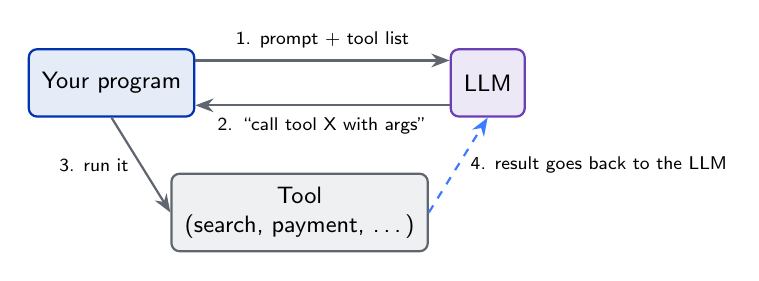
\begin{tikzpicture}[node distance=7mm and 12mm,scale=0.95,transform shape]
  \node[actor] (app) {Your program};
  \node[agent,right=34mm of app] (llm) {LLM};
  \node[service,below=12mm of $(app)!0.5!(llm)$] (tool) {Tool\\(search, payment, \dots)};
  \draw[flow] ([yshift=3mm]app.east) -- node[lbl,above=1mm] {1. prompt + tool list} ([yshift=3mm]llm.west);
  \draw[flow] ([yshift=-3mm]llm.west) -- node[lbl,below=1mm] {2. ``call tool X with args''} ([yshift=-3mm]app.east);
  \draw[flow] (app.south) -- node[lbl,left=1mm] {3. run it} (tool.west);
  \draw[data] (tool.east) -- node[lbl,right=1mm] {4. result goes back to the LLM} (llm.south);
\end{tikzpicture}
\end{center}

\subsection{Vision models}
A \term{vision model} is an LLM that can also take images as input. You send a photo plus a question and receive text. This is how a program can ``read'' a price tag, a receipt or a shop shelf. Vision models can misread blurry or small text, so a careful design lets the model only \emph{read} and lets ordinary code \emph{decide}. Shelfie follows this rule (Chapter~8).

\section{From model to agent}

An \term{AI agent} is a program that uses an LLM to pursue a \emph{goal} over several steps, choosing and using tools on its own. Instead of one question and one answer, it runs a loop.

\begin{center}
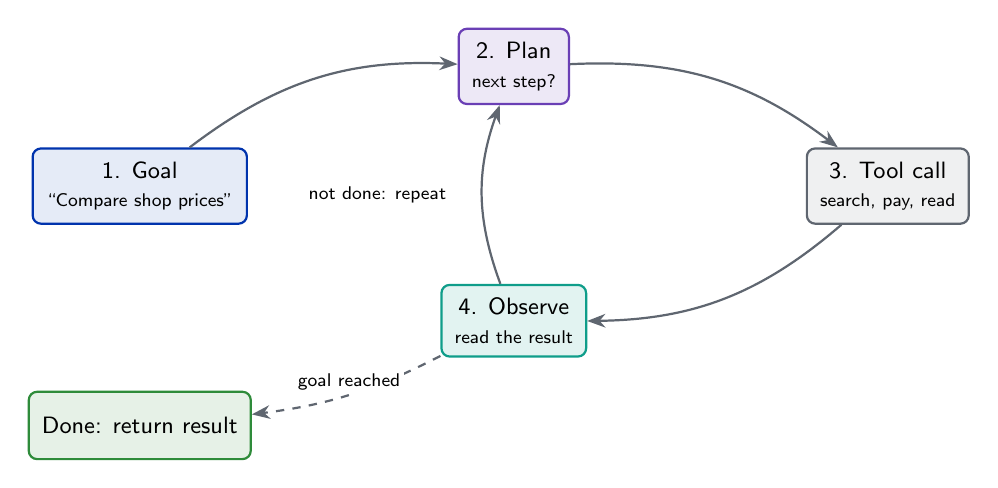
\begin{tikzpicture}[scale=0.95,transform shape]
  \node[actor] (goal) at (0,0) {1. Goal\\{\scriptsize ``Compare shop prices''}};
  \node[agent] (plan) at (5,1.6) {2. Plan\\{\scriptsize next step?}};
  \node[service] (act) at (10,0) {3. Tool call\\{\scriptsize search, pay, read}};
  \node[chain] (obs) at (5,-1.8) {4. Observe\\{\scriptsize read the result}};
  \draw[flow] (goal) to[bend left=20] (plan);
  \draw[flow] (plan) to[bend left=20] (act);
  \draw[flow] (act) to[bend left=20] (obs);
  \draw[flow] (obs) to[bend left=20] node[lbl,pos=0.5,xshift=-14mm] {not done: repeat} (plan);
  \node[good] (done) at (0,-3.2) {Done: return result};
  \draw[flow,dashed] (obs) to[bend left=10] node[lbl,above] {goal reached} (done);
\end{tikzpicture}
\end{center}

\subsection{Agent, chatbot or script?}
\begin{center}
\small
\begin{tabularx}{\textwidth}{@{}p{3.1cm}XXX@{}}
\toprule
 & \textbf{Plain script} & \textbf{Chatbot} & \textbf{AI agent} \\
\midrule
Who decides the steps? & The programmer, fixed in advance & A human, one message at a time & The model, at run time \\
Uses tools? & Yes, hard-coded & Usually no & Yes, chosen by the model \\
Handles surprises? & No, it breaks & Answers in text only & Can retry or change plan \\
Loops until done? & Only if coded & No, waits for the user & Yes \\
Predictable? & Very & Medium & Least; needs guard rails \\
Example & Nightly price scraper & Support chat window & Research bot that searches, reads, pays for data and writes a report \\
\bottomrule
\end{tabularx}
\end{center}

\begin{warningbox}{``Agent'' is a loose word}
In marketing almost anything is called an agent. For this guide: an agent has a goal, a loop, and tools with real effects (spending money, sending messages). The more real effects, the more guard rails it needs. The best agent design is often a mix: the model handles the fuzzy part, plain code handles the checks and the money.
\end{warningbox}

\section{Agentic commerce}

\term{Agentic commerce} means software agents taking part in buying and selling: an agent \emph{sells} a service (writes a report, answers a data query), an agent \emph{buys} a service (pays for a dataset or a specialist), and sometimes an agent buys from or sells to humans. The track's own description is an agent, service or developer tool that does useful work and \emph{charges for it on Cardano}.

\subsection{Three patterns}
\begin{center}
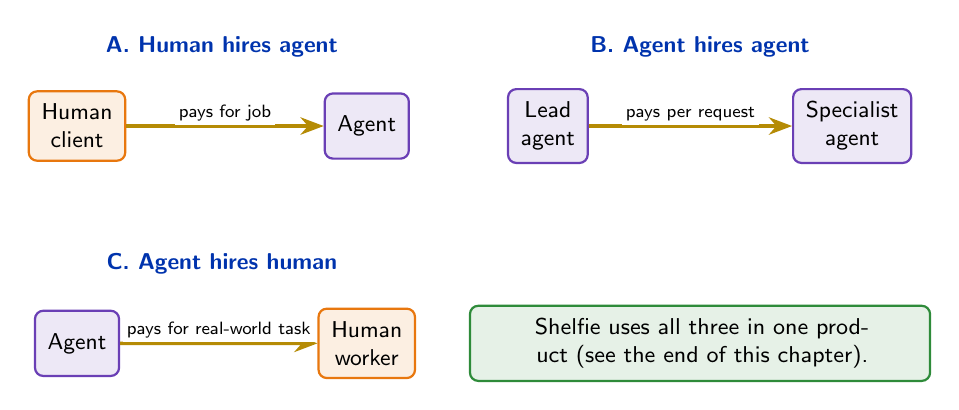
\begin{tikzpicture}[scale=0.92,transform shape,node distance=6mm]
  % pattern A
  \node[human] (a1) at (0,0) {Human\\client};
  \node[agent] (a2) at (4,0) {Agent};
  \draw[pay] (a1) -- node[lbl,above] {pays for job} (a2);
  \node[font=\sffamily\small\bfseries,color=cBlue] at (2,1.1) {A. Human hires agent};
  % pattern B
  \node[agent] (b1) at (6.5,0) {Lead\\agent};
  \node[agent] (b2) at (10.7,0) {Specialist\\agent};
  \draw[pay] (b1) -- node[lbl,above] {pays per request} (b2);
  \node[font=\sffamily\small\bfseries,color=cBlue] at (8.6,1.1) {B. Agent hires agent};
  % pattern C
  \node[agent] (c1) at (0,-3) {Agent};
  \node[human] (c2) at (4,-3) {Human\\worker};
  \draw[pay] (c1) -- node[lbl,above] {pays for real-world task} (c2);
  \node[font=\sffamily\small\bfseries,color=cBlue] at (2,-1.9) {C. Agent hires human};
  \node[good,text width=6cm] at (8.6,-3) {Shelfie uses all three in one product (see the end of this chapter).};
\end{tikzpicture}
\end{center}

Pattern C is the unusual one: a software agent can pay a person to do something it cannot, such as photographing a shelf in a physical shop. Cardano's brief explicitly mentions agents that ``act in the real world by buying, publishing or booking''.

\subsection{Why an agent needs its own money, identity and receipts}
A human pays with a bank card tied to a name and a monthly statement. An agent has none of that, and sharing a person's card with a program is dangerous. So an agent economy needs:
\begin{itemize}
  \item \textbf{Its own wallet.} A cryptographic account the agent controls, funded with a small budget. No bank account or sign-up is needed.
  \item \textbf{An identity.} Others must know \emph{which} agent they are dealing with, so that reputation and responsibility attach to something. Masumi stores agent registrations on-chain (below).
  \item \textbf{Receipts.} A payment that anyone can verify later: who paid whom, how much, for which job. On a blockchain every payment is automatically such a receipt.
  \item \textbf{Spending limits.} The agent should never be able to spend more than a cap per payment and per job.
  \item \textbf{Conditional payment.} For a job that takes time, money should be held until the work is delivered (\emph{escrow}, explained below).
\end{itemize}

\begin{analogybox}{Company credit card with a limit}
Give an intern a company card with a 50 EUR limit and receipts required. The intern can buy supplies without asking you each time, and the worst case is 50 EUR. A wallet with a spending cap works the same way for an agent.
\end{analogybox}

\subsection{Risks}
\begin{center}
\small
\begin{tabularx}{\textwidth}{@{}p{3.2cm}XX@{}}
\toprule
\textbf{Risk} & \textbf{What can go wrong} & \textbf{Typical countermeasure} \\
\midrule
Runaway spending & A loop keeps buying data; a bug or a prompt trick drains the wallet & Per-payment cap, small throw-away wallet, job budget \\
Fraud & A seller takes money and returns junk; a buyer claims non-delivery & Escrow with refund; automatic checks before release \\
Accountability & Nobody knows who is responsible for a bad action by an agent & Registered identity, recorded decisions and hashes \\
Prompt injection & Text on a web page tells the agent to pay someone & Code-level limits that the model cannot override \\
Bad output accepted as good & The LLM judges its own work too generously & Deterministic pass/fail rules, not model opinion \\
\bottomrule
\end{tabularx}
\end{center}

\section{The track brief, explained}

Source: the official prize page of the hackathon, copied into the team's research file of 29 October 2026. The table below restates it.

\begin{center}
\small
\begin{tabularx}{\textwidth}{@{}p{3.4cm}X@{}}
\toprule
\textbf{Item} & \textbf{What the brief says} \\
\midrule
Challenge & An agent, service or developer tool that does a useful job and \emph{charges for it on Cardano}. \\
Prizes & Total 6,000 EUR: 1st \textbf{3,000 EUR}, 2nd \textbf{2,000 EUR}, 3rd \textbf{1,000 EUR}. \\
Two payment routes (may be combined) & \textbf{Per job: Masumi on Sokosumi.} The agent becomes a hireable ``Coworker''; the payment waits in escrow until delivery, with a refund if nothing is delivered.\newline \textbf{Per request: x402.} HTTP~402, no accounts or API keys; called ``the fastest way to a first payment''. \\
\textbf{Hard requirement} & A working agent or service that completes \textbf{at least one paid job or payment on Cardano preprod}, via Masumi or x402. (Preprod is the free test network; see Chapter~2.) \\
Extra to hand in & The \textbf{transaction hash} of that preprod payment; a video of at most 2.5 minutes saying who it is for, the problem, the \textbf{business case}, and one paid job from start to finish; a description of how it works, which Cardano tools it uses and how it could run in real life. \\
Judging criteria & Original use case; complete paid workflow; technical execution with Cardano tools; creativity; user experience; pitch and demo; real-world impact and continuity after the hackathon. \\
What Cardano especially wants to see & (1) A clear \textbf{customer and their journey}; (2) \textbf{payment tied to the result}: escrow, refunds, or paying only for work that passed a check; (3) \textbf{agents hiring other agents}, or agents acting in the real world; (4) a \textbf{live demo} with the transaction visible on a preprod explorer. \\
Judges & Bora Oben (Cardano) and Vladislav Kudrin (Cardano Foundation). \\
Timing & Hacking starts Fri 30 Oct, 09:00; submission deadline Sat 31 Oct, 15:00; live judging 15:00--17:00; winners 17:30. \\
\bottomrule
\end{tabularx}
\end{center}

\begin{center}
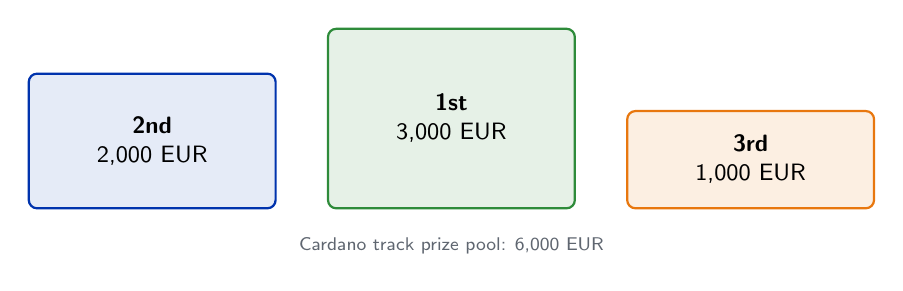
\begin{tikzpicture}[scale=0.95,transform shape]
  \node[good,minimum width=3.3cm,minimum height=2.4cm] (p1) at (0,0) {\textbf{1st}\\3,000 EUR};
  \node[actor,minimum width=3.3cm,minimum height=1.8cm] (p2) at (-4,-0.3) {\textbf{2nd}\\2,000 EUR};
  \node[human,minimum width=3.3cm,minimum height=1.3cm] (p3) at (4,-0.55) {\textbf{3rd}\\1,000 EUR};
  \node[font=\sffamily\scriptsize,color=cGrey] at (0,-1.7) {Cardano track prize pool: 6,000 EUR};
\end{tikzpicture}
\end{center}

\begin{warningbox}{A completed task is not a payment}
The Masumi guide warns that a Sokosumi task showing \code{COMPLETED} does \emph{not} prove that a payment happened. We must show the seller's receipt and the transaction hash. Without the hash we have not met the hard requirement.
\end{warningbox}

\begin{shelfiebox}{Our route to the requirement}
The team's plan treats x402 as the fast, low-risk way to qualify (one paid request) and Masumi escrow as the heavier second layer that earns the ``pay on result'' points. If the escrow is not working by Friday 22:00 it is frozen and shown as roadmap; the x402 payment still satisfies the requirement.
\end{shelfiebox}

\section{Masumi Network}

\term{Masumi} is a network for agent payments and agent identity on Cardano. It gives agent developers the pieces that are hard to build alone: a way to get paid per job, hold payment in escrow, register an agent publicly, and keep tamper-proof records of what an agent did. Think of it as the payment and trust layer, while \term{Sokosumi} (next section) is the marketplace on top where people hire agents.

\begin{center}
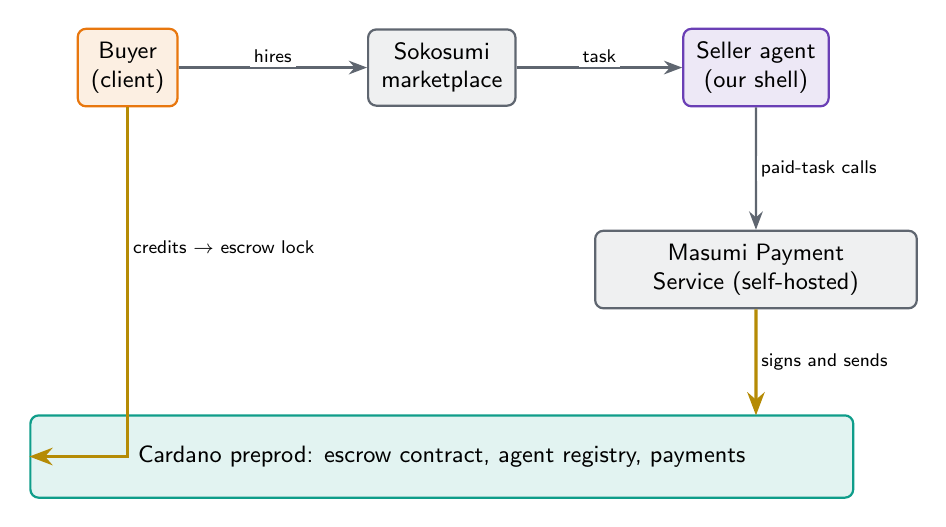
\begin{tikzpicture}[scale=0.95,transform shape]
  \node[human] (buyer) at (0,0) {Buyer\\(client)};
  \node[service] (soko) at (4.2,0) {Sokosumi\\marketplace};
  \node[agent] (agent) at (8.4,0) {Seller agent\\(our shell)};
  \node[service,minimum width=4.3cm] (mps) at (8.4,-2.7) {Masumi Payment\\Service (self-hosted)};
  \node[chain,minimum width=11cm,minimum height=1.1cm] (cardano) at (4.2,-5.2) {Cardano preprod: escrow contract, agent registry, payments};
  \draw[flow] (buyer) -- node[lbl,above] {hires} (soko);
  \draw[flow] (soko) -- node[lbl,above] {task} (agent);
  \draw[flow] (agent) -- node[lbl,right] {paid-task calls} (mps);
  \draw[pay] (mps) -- node[lbl,right] {signs and sends} (8.4,-4.65);
  \draw[pay] (buyer) |- node[lbl,pos=0.2,right] {credits $\rightarrow$ escrow lock} (cardano.west);
\end{tikzpicture}
\end{center}

\subsection{The Masumi Payment Service}
The \term{Masumi Payment Service} (MPS) is the software that talks to the blockchain for an agent: it holds the seller wallet, registers the agent, watches for a buyer's escrow payment, submits result hashes and withdraws the earnings. The hackathon requires us to \emph{run our own copy}; it is not a hosted service. According to the runbook:
\begin{itemize}
  \item \textbf{Node.js} at least 24.22.1 and below 25 (Node 26 is not supported).
  \item \textbf{pnpm} version 10.30.2 (the package manager the project is pinned to).
  \item \textbf{PostgreSQL} 13 or newer (15 recommended) as its database; on a laptop with only the \code{psql} client, run Postgres in Docker.
  \item \textbf{Seeded wallets}: a seed script creates wallets and prints their secret recovery phrases once. Only the operator may see them; never record or commit them.
  \item A free \textbf{Blockfrost} preprod API key (the service that reads the chain) and secrets in a private \code{.env} file (database URL, encryption key of at least 32 characters, admin key).
  \item Default port 38127, with an admin page and API docs on the same address.
\end{itemize}
Test money comes from the Masumi dispenser (tADA and test dollar tokens). The runbook also mentions a quote of 1 test USDM for the sample task and a separate optional 5~ADA collateral from the dispenser; both are things to confirm on Friday.

\subsection{Agent registry and decision logging}
Before an agent can sell on Masumi it is \term{registered on-chain}. The registration creates a public record (an NFT, according to the research notes) that ties together the agent's identifier, its owner wallet (the seller verification key) and its payment settings. A buyer, a marketplace or a judge can look it up; nobody can quietly swap the identity. In the starter, a script registers the agent and you repeat a status read until it says \code{RegistrationConfirmed}; the confirmed identifier then goes into a state file.

\term{Decision logging} is the companion idea: instead of storing a whole report on the chain (expensive), the agent records a \term{hash} (a fixed-length fingerprint, Chapter~1) of its result. Anyone who later holds the report can recompute the hash and compare. If one character changed, the hashes differ. This gives an audit trail of ``what this agent delivered'' without putting the content on-chain.

\subsection{Escrow and its lifecycle}
\term{Escrow} means a neutral holder keeps the buyer's money until the seller delivers. On Masumi the neutral holder is a smart contract on Cardano. The buyer locks funds (\code{FundsLocked}); the seller does the work and submits a result hash (\code{ResultSubmitted}); after a waiting period the seller can withdraw. If the seller submits nothing before the deadline, the buyer can get the money back.

\begin{analogybox}{Holding a deposit with a notary}
You hire a photographer. You hand the fee to a notary. When the photos arrive, the notary pays the photographer; if they never arrive, the notary returns your money. Neither side has to trust the other, only the notary. Here the notary is code that nobody can bribe.
\end{analogybox}

The contract uses several deadlines. The runbook gives these offsets (all \emph{estimates} derived from reading the code, counted from the start of the job): pay by $+5$~min, submit the result by $+20$~min, unlock at $+36$~min, an external-dispute unlock at $+52$~min. Automatic seller withdrawal needs a result hash plus ten more minutes after unlock (about $+46$), and an automatic buyer refund applies if no hash exists ten minutes after the submit deadline (about $+30$). A complete paid cycle takes \textbf{at least 60 minutes} including on-chain confirmations.

\begin{center}
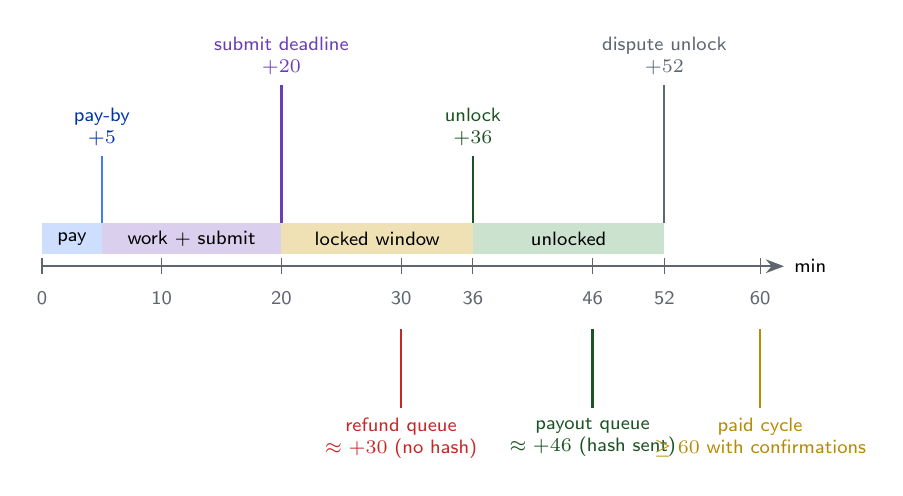
\begin{tikzpicture}[x=0.152cm,y=1cm,font=\sffamily\scriptsize]
  % axis 0..60 minutes
  \draw[thick,->,draw=cGrey] (0,0) -- (62,0) node[right] {min};
  \foreach \x in {0,10,20,30,36,46,52,60}{\draw[draw=cGrey] (\x,0.1) -- (\x,-0.1);}
  \foreach \x in {0,10,20,30,36,46,52,60}{\node[below=1mm,color=cGrey] at (\x,-0.1) {\x};}
  % phases
  \fill[cSky!25] (0,0.15) rectangle (5,0.55);
  \fill[cPurple!25] (5,0.15) rectangle (20,0.55);
  \fill[cGold!30] (20,0.15) rectangle (36,0.55);
  \fill[cGreen!25] (36,0.15) rectangle (52,0.55);
  \node at (2.5,0.35) {pay};
  \node at (12.5,0.35) {work + submit};
  \node at (28,0.35) {locked window};
  \node at (44,0.35) {unlocked};
  % milestones above
  \draw[thick,draw=cSky] (5,0.55) -- (5,1.4) node[above,align=center,color=cBlue] {pay-by\\$+5$};
  \draw[thick,draw=cPurple] (20,0.55) -- (20,2.3) node[above,align=center,color=cPurple] {submit deadline\\$+20$};
  \draw[thick,draw=cGreen!60!black] (36,0.55) -- (36,1.4) node[above,align=center,color=cGreen!60!black] {unlock\\$+36$};
  \draw[thick,draw=cGrey] (52,0.55) -- (52,2.3) node[above,align=center,color=cGrey] {dispute unlock\\$+52$};
  % estimates below
  \draw[thick,draw=cRed] (30,-0.8) -- (30,-1.8) node[below,align=center,color=cRed] {refund queue\\$\approx +30$ (no hash)};
  \draw[thick,draw=cGreen!60!black] (46,-0.8) -- (46,-1.8) node[below,align=center,color=cGreen!60!black] {payout queue\\$\approx +46$ (hash sent)};
  \draw[thick,draw=cGold!90!black] (60,-0.8) -- (60,-1.8) node[below,align=center,color=cGold!90!black] {paid cycle\\$\geq 60$ with confirmations};
\end{tikzpicture}
\end{center}
{\footnotesize\textcolor{cGrey}{All offsets are estimates from the runbook (counted from the start of the job). The exact reference point and whether the buyer-side refund runs automatically must be confirmed Friday with the Masumi engineer.}}

\begin{warningbox}{The crucial rule: any submitted hash pays the seller}
The escrow cannot judge quality. If the seller submits \emph{any} result hash, even for a text that says ``failed'', the contract treats the job as delivered and the seller can be paid. Marking the Sokosumi task as failed does \emph{not} trigger a refund. To refund the buyer after a failed job, the seller must \textbf{withhold the result}: persist the failure locally, submit no hash, do not complete the task, and explain the reason in the task text. The buyer's no-result timeout then returns the money. The alternative, a manual refund request followed by the seller's authorisation, also exists but needs the buyer's side.
\end{warningbox}

\begin{center}
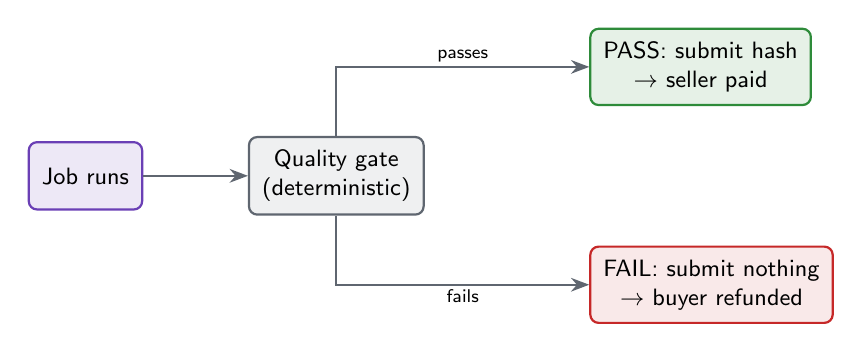
\begin{tikzpicture}[scale=0.95,transform shape,node distance=8mm and 10mm]
  \node[agent] (job) {Job runs};
  \node[service,right=14mm of job] (gate) {Quality gate\\(deterministic)};
  \node[good,above right=4mm and 22mm of gate] (pass) {PASS: submit hash\\$\rightarrow$ seller paid};
  \node[bad,below right=4mm and 22mm of gate] (fail) {FAIL: submit nothing\\$\rightarrow$ buyer refunded};
  \draw[flow] (job) -- (gate);
  \draw[flow] (gate) |- node[lbl,pos=0.75,above] {passes} (pass);
  \draw[flow] (gate) |- node[lbl,pos=0.75,below] {fails} (fail);
\end{tikzpicture}
\end{center}

\subsection{Seeing a Masumi job as a state machine}
A \term{state machine} is a diagram of the states a thing can be in and the events that move it between them. This is a simplified view of one paid job. State names with a monospaced font appear in the runbook; the others are our plain-language labels.

\begin{center}
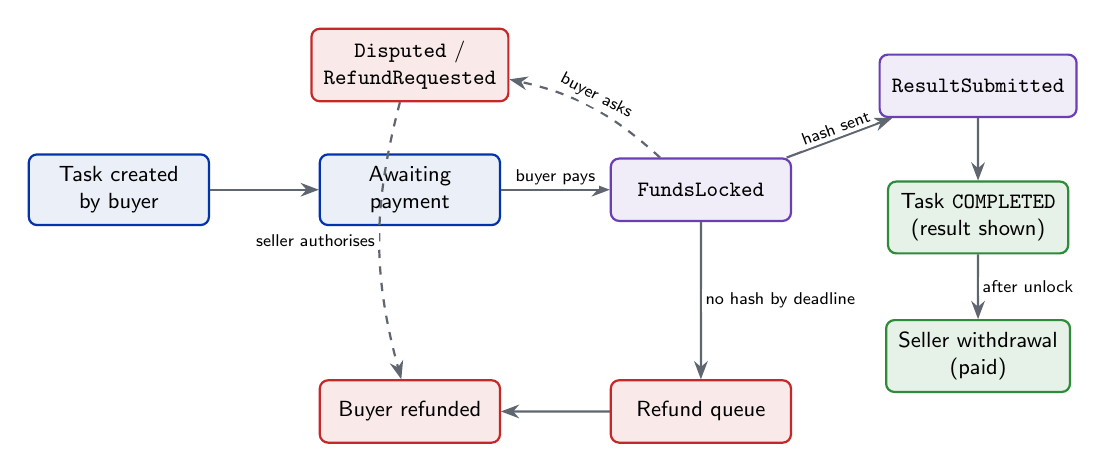
\begin{tikzpicture}[scale=0.88,transform shape,
  st/.style={box,minimum width=2.6cm,fill=cBlue!8,draw=cBlue},
  stg/.style={box,minimum width=2.6cm,fill=cGreen!12,draw=cGreen},
  str/.style={box,minimum width=2.6cm,fill=cRed!10,draw=cRed},
  stp/.style={box,minimum width=2.6cm,fill=cPurple!10,draw=cPurple}]
  \node[st] (req) at (0,0) {Task created\\by buyer};
  \node[st] (await) at (4.2,0) {Awaiting\\payment};
  \node[stp] (locked) at (8.4,0) {\code{FundsLocked}};
  \node[stp] (sub) at (12.4,1.5) {\code{ResultSubmitted}};
  \node[stg] (comp) at (12.4,-0.4) {Task \code{COMPLETED}\\(result shown)};
  \node[stg] (paid) at (12.4,-2.4) {Seller withdrawal\\(paid)};
  \node[str] (ref) at (8.4,-3.2) {Refund queue};
  \node[str] (refd) at (4.2,-3.2) {Buyer refunded};
  \node[str] (disp) at (4.2,1.8) {\code{Disputed} /\\\code{RefundRequested}};
  \draw[flow] (req) -- (await);
  \draw[flow] (await) -- node[lbl,above] {buyer pays} (locked);
  \draw[flow] (locked) -- node[lbl,above,sloped] {hash sent} (sub);
  \draw[flow] (sub) -- (comp);
  \draw[flow] (comp) -- node[lbl,right] {after unlock} (paid);
  \draw[flow] (locked) -- node[lbl,right] {no hash by deadline} (ref);
  \draw[flow] (ref) -- (refd);
  \draw[flow,dashed] (locked) to[bend right=15] node[lbl,above,sloped] {buyer asks} (disp);
  \draw[flow,dashed] (disp) to[bend right=15] node[lbl,left] {seller authorises} (refd);
\end{tikzpicture}
\end{center}
{\footnotesize\textcolor{cGrey}{Simplified: the real contract has more intermediate and error states (for example \code{Withdrawn}, pending confirmations, cooldowns).}}

\subsection{The x402 path inside Masumi}
Besides the Sokosumi credit route, the team's open questions list a variant where a headless agent pays \emph{into} a Masumi escrow using x402, through a \code{/x402/start\_job} path. We have not verified how it works; it is on the list of questions for the Masumi engineer on Friday. The design decision records note it as a 4+ hour option to attempt only if time remains. Treat it as unconfirmed.

\section{Sokosumi}

\term{Sokosumi} is the agent marketplace in the Masumi world: a web app where people hire AI ``coworkers'' for tasks and pay in credits. It was launched by Serviceplan Group with NMKR; the public page lists eight coworkers (for example a research coworker and a coding coworker), mostly generic roles. For the hackathon there is a free test version at \code{preprod.sokosumi.com} and a shared team space called the \textbf{TUM Workspace} that every participant must join.

\subsection{Vendor, Coworker, worker}
\begin{center}
\small
\begin{tabularx}{\textwidth}{@{}p{2.8cm}X@{}}
\toprule
\textbf{Concept} & \textbf{Meaning} \\
\midrule
\term{Vendor} & The company-like account that offers agents. One per account; it needs organisation membership first. In our plan it is our team's seller identity. \\
\term{Coworker} & The agent as it appears to customers: a name, a description, and the kinds of tasks it accepts. Ours is a \emph{private} Coworker during development. \\
\term{Worker process} & The program running on a laptop that \emph{polls} Sokosumi every few seconds for new tasks for the Coworker, runs the agent and posts the result. Start it with \code{npm run worker}. \\
\term{Task} & One request from a buyer to a Coworker. It moves through statuses such as \code{READY} and \code{COMPLETED}. \\
\bottomrule
\end{tabularx}
\end{center}

\begin{center}
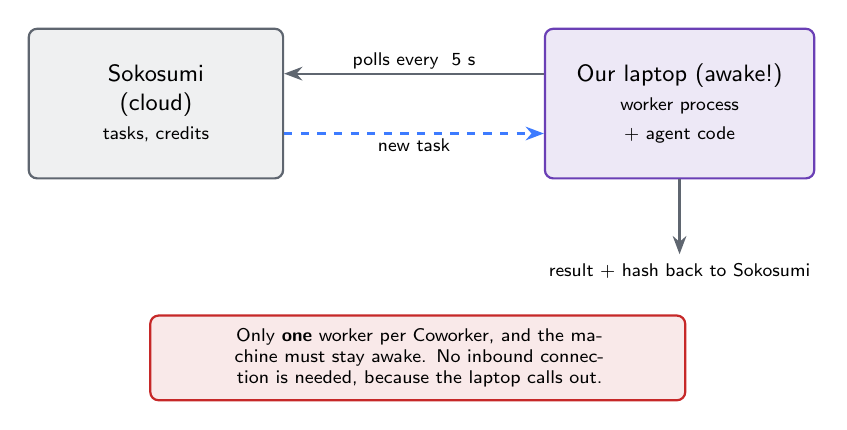
\begin{tikzpicture}[scale=0.95,transform shape]
  \node[service,minimum width=3.4cm,minimum height=2cm] (soko) at (0,0) {Sokosumi\\(cloud)\\{\scriptsize tasks, credits}};
  \node[agent,minimum width=3.6cm,minimum height=2cm] (laptop) at (7,0) {Our laptop (awake!)\\{\scriptsize worker process}\\{\scriptsize + agent code}};
  \draw[flow] ([yshift=4mm]laptop.west) -- node[lbl,above] {polls every ~5 s} ([yshift=4mm]soko.east);
  \draw[data] ([yshift=-4mm]soko.east) -- node[lbl,below] {new task} ([yshift=-4mm]laptop.west);
  \draw[flow] (laptop.south) -- ++(0,-1) node[below,font=\sffamily\scriptsize] {result + hash back to Sokosumi};
  \node[bad,text width=6.8cm,font=\sffamily\scriptsize] at (3.5,-3.4) {Only \textbf{one} worker per Coworker, and the machine must stay awake. No inbound connection is needed, because the laptop calls out.};
\end{tikzpicture}
\end{center}

\subsection{The \code{sokosumi} command-line tool}
Each team member installs the official command-line tool, package \code{@masumi\_network/sokosumi} version \textbf{1.0.4}, under Node 24. Typical first commands (preprod flag, as in the runbook):
\begin{lstlisting}
sokosumi --preprod auth login
sokosumi --preprod auth whoami --json
sokosumi --preprod workspaces list --json
\end{lstlisting}
Logging in opens the browser. On Linux the tool stores its credentials in the operating system's secret store, so a keyring service (for example GNOME Keyring) must be running. A human login is different from the key the running agent uses (the runtime key is stored separately).

\subsection{Credits versus on-chain payments}
\begin{conceptbox}{Sokosumi credits are not x402}
Buyers on Sokosumi pay with \term{credits}, an account balance inside the platform. When a paid Masumi job runs, the platform converts credits into the escrow lock on-chain. But if our lead agent hires \emph{another} Sokosumi agent through the platform, it again pays in credits, which gives us no transaction hash we control. For the track we want a real on-chain payment between agents, so we use \textbf{x402} for that leg. The runbook states this directly: Sokosumi credits $\neq$ x402.
\end{conceptbox}

\subsection{The starter and model keys}
The organisers provide a starter repository called \code{tum-hackathon-quickstart}, pinned in the runbook to a specific commit. It contains the agent definition, the worker, the paid-task adapter and a settlement checker. Its agent needs access to an LLM provider, configured through environment variables: \code{ZAI\_API\_KEY}, \code{ZAI\_BASE\_URL}, \code{ZAI\_MODEL} and optionally \code{ZAI\_CONTEXT\_WINDOW\_TOKENS}. The guide suggests Z.ai or Vercel AI Gateway; another provider means adapting the agent code. Two terminals are used: \code{npm start} (the agent runtime) and \code{npm run worker}, until the log says ``Continuous worker running''.

\begin{examplebox}{From clone to first paid task (runbook order)}
\begin{enumerate}[nosep]
  \item Install Node 24 and the Sokosumi CLI; sign up on preprod Sokosumi; join the TUM Workspace.
  \item Create Vendor and private Coworker; connect it; import its key into the OS vault.
  \item Run the agent and worker; create a smoke task; see \code{COMPLETED} (\emph{no payment yet}, 5--15 min).
  \item Start the Masumi Payment Service, fund the seller wallet from the dispenser (15--30 min), register the agent until \code{RegistrationConfirmed}.
  \item Set \code{PAID\_TASKS\_ENABLED=true}, restart the worker. If registration is not ready it silently falls back to an \emph{unpaid} task, so verify.
  \item Run a fresh task: credits $\rightarrow$ \code{FundsLocked} $\rightarrow$ result hash $\rightarrow$ \code{ResultSubmitted} $\rightarrow$ \code{COMPLETED}, then fetch the receipt. Allow at least 60 min.
  \item Paste the receipt's transaction hash into the preprod Cardanoscan explorer and save the URL.
\end{enumerate}
\end{examplebox}

\section{What already exists: the competitive landscape}

The team's research (public sources only, some pages unreachable) found this picture.
\begin{itemize}
  \item \textbf{On the marketplace:} generic research, marketing and coding agents. The hackathon template and the track's own example (a research report for a shop) push every team towards a generic research agent, so this is the most crowded space. Likely empty (an inference, unverified): agents doing a checkable real-world task for a small customer, and agents that buy from other agents with a proof-of-result gate.
  \item \textbf{Past hackathons:} winners were infrastructure or a clear new commerce primitive (pay per tool call, getting past paywalls, guest checkout), showed a \emph{real} transaction rather than a mock, and told a concrete story for a specific audience.
  \item \textbf{The x402 on Cardano path} is new: the Cardano Foundation contributed the Cardano support, and its hosted test facilitator has run only on preprod. Critics note there is little evidence of agents paying for real services in ADA at volume, so a visible real-commerce example is valuable.
\end{itemize}

\begin{center}
\small
\begin{tabularx}{\textwidth}{@{}XX@{}}
\toprule
\textbf{Most teams will} & \textbf{How we can stand out (inference)} \\
\midrule
Build a generic research/summary agent on the template & Named customer with real pain and a price that fits \\
Show a ``pay'' button without a transaction hash & Outcome-gated payment with a recorded refund \\
Show only the happy path & A deterministic checker (rules) decides pass/fail \\
Pitch ``the agent economy'' in general & One agent hiring another with a spend cap, visible in a live ledger; explorer links in the demo \\
\bottomrule
\end{tabularx}
\end{center}

\begin{conceptbox}{The lesson we took}
\textbf{Lesson:} escrow-with-refund works best when a \emph{deterministic pass/fail gate} decides, not an LLM opinion.
\end{conceptbox}

\section{How Shelfie uses each piece}

\begin{shelfiebox}{The lead agent: a Sokosumi Coworker with Masumi escrow}
A brand manager hires Shelfie on Sokosumi (``check this product in N stores, at least K must pass''). The fee is locked in Masumi escrow. Our \emph{shell} (a thin fork of the quickstart) runs the worker, receives the paid task and hands it to our engine. When the engine decides, the shell either submits the report hash (seller paid) or, on a failed K-of-N result, \textbf{withholds the result} so the brand is refunded after the timeout. The shell holds no business logic; it is one bridge file.
\end{shelfiebox}

\begin{shelfiebox}{The verifier agent: paid via x402}
The verifier is a separate service that sells \code{POST /v1/verify} behind x402 at 1~tADA per check. Our engine pays it from a dedicated buyer wallet (with a per-payment spending cap) every time a worker submits a photo. Every check, pass or fail, is therefore a visible on-chain payment: agent pays agent. Sokosumi credits were rejected for this leg because they give no hash we control.
\end{shelfiebox}

\begin{shelfiebox}{Humans: paid by plain transfer}
When the verifier passes a photo, the engine pays the human worker a bounty by an ordinary Cardano transfer from a payout wallet. Escrow per worker would take at least an hour and x402 would need a seller on every phone, so a plain transfer is the decision (with fallbacks if the library cannot build the transfer: to verify Friday).
\end{shelfiebox}

\begin{center}
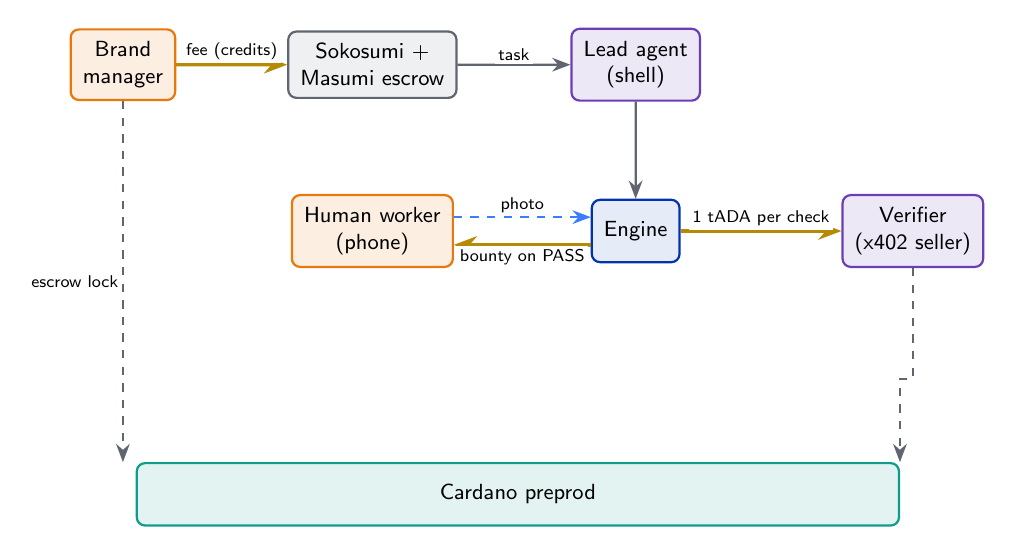
\begin{tikzpicture}[scale=0.88,transform shape]
  \node[human] (brand) at (0,3) {Brand\\manager};
  \node[service] (soko) at (3.6,3) {Sokosumi +\\Masumi escrow};
  \node[agent] (shell) at (7.4,3) {Lead agent\\(shell)};
  \node[actor] (engine) at (7.4,0.6) {Engine};
  \node[agent] (ver) at (11.4,0.6) {Verifier\\(x402 seller)};
  \node[human] (work) at (3.6,0.6) {Human worker\\(phone)};
  \node[chain,minimum width=11cm] (ch) at (5.7,-3.2) {Cardano preprod};
  \draw[pay] (brand) -- node[lbl,above] {fee (credits)} (soko);
  \draw[flow] (soko) -- node[lbl,above] {task} (shell);
  \draw[flow] (shell) -- (engine);
  \draw[pay] (engine) -- node[lbl,above] {1 tADA per check} (ver);
  \draw[pay] ([yshift=-2mm]engine.west) -- node[lbl,below] {bounty on PASS} ([yshift=-2mm]work.east);
  \draw[data] ([yshift=2mm]work.east) -- node[lbl,above] {photo} ([yshift=2mm]engine.west);
  \draw[flow,dashed] (brand.south) -- node[lbl,left] {escrow lock} (brand.south |- ch.north);
  \draw[flow,dashed] (ver.south) -- ++(0,-1.6) -| (ch.north east);
\end{tikzpicture}
\end{center}
{\footnotesize\textcolor{cGrey}{Simplified overview: the photo actually goes from the worker page to the engine (Chapter~7 shows the exact flows). Pattern A = brand hires agent, B = engine/lead agent pays verifier, C = agent pays human.}}

\begin{center}
\small
\begin{tabularx}{\textwidth}{@{}p{3.2cm}p{3.8cm}X@{}}
\toprule
\textbf{Payment} & \textbf{Mechanism} & \textbf{Why} \\
\midrule
Brand $\rightarrow$ Shelfie & Sokosumi credits into Masumi escrow & Pay on result; refund if K-of-N fails \\
Engine $\rightarrow$ verifier & x402, 1 tADA per check & Agent-to-agent payment with a tx hash we control \\
Engine $\rightarrow$ worker & Plain Cardano transfer & Fast, cheap, no extra protocol \\
\bottomrule
\end{tabularx}
\end{center}

\begin{warningbox}{Be honest about the limits}
Escrow settlement takes an hour or more, so on stage we show the live x402 and payout legs and present settlement and refund from earlier recorded runs, clearly labelled. No code is built yet; everything above is the plan.
\end{warningbox}

\begin{keypoints}
\begin{itemize}[nosep]
\item An AI agent is an LLM in a loop (goal, plan, tool call, observe, repeat) with tools that have real effects; it needs its own wallet, identity, receipts and spending limits.
\item The Cardano track pays 3,000 / 2,000 / 1,000 EUR and has one hard requirement: at least one paid job or payment on \textbf{preprod}, via Masumi or x402, proven by a transaction hash.
\item Masumi = payment and identity layer (self-hosted Payment Service, on-chain registry, escrow); Sokosumi = the marketplace where Coworkers are hired with credits.
\item Escrow cannot judge quality: \textbf{any submitted result hash pays the seller}. A failed job must withhold the result so the buyer is refunded after the timeout.
\item A paid Masumi cycle takes at least 60 minutes; plan for it and record refund and settlement runs before the demo.
\item Sokosumi credits are not x402. Shelfie uses escrow for the brand, x402 for the verifier and plain transfers for humans.
\end{itemize}
\end{keypoints}

\begin{quizbox}
\begin{enumerate}[nosep]
  \item What are the four steps of the agent loop, and what makes an agent different from a script?
  \item What is the single hard requirement of the Cardano track, and what must be handed in as proof?
  \item In escrow, what happens if the seller submits a result hash for a failed job? How must a failed job be handled to refund the buyer?
  \item Name the three things you need to run the Masumi Payment Service besides its code.
  \item Why does Shelfie pay its verifier with x402 rather than with Sokosumi credits?
  \item Why can the escrow settlement not be shown live on stage?
\end{enumerate}
\medskip
{\footnotesize\color{cGrey}\textbf{Answers.} 1: goal/plan, tool call, observe, repeat; the model chooses the steps at run time. 2: at least one paid job or payment on Cardano preprod (Masumi or x402); the transaction hash. 3: the seller is paid; withhold the result (no hash, no completion) and let the no-result timeout refund. 4: Node 24.22.x with pnpm 10.30.2, a PostgreSQL database, seeded wallets (plus a Blockfrost preprod key). 5: credits give no transaction hash we control; x402 gives an on-chain payment between agents. 6: a paid cycle takes at least 60 minutes, so we show recorded runs with explorer links.}
\end{quizbox}

\chapter{On-chain versus off-chain}

\section*{Why this matters for us}
A common mistake in blockchain projects is to put everything on the chain, or nothing. Shelfie does neither on purpose. Photos, verdicts, the database and the vision model stay on our own servers; money movements and the escrow that protects the customer live on the Cardano chain. Judges will ask ``what is actually on-chain?'' and ``who do I have to trust?''. This chapter gives you the vocabulary and the honest answers, including the escrow timing facts that decide how we design the demo.

\section{Two zones}
\begin{conceptbox}{On-chain and off-chain}
\term{On-chain} means recorded in the blockchain itself: every node stores it and anyone can read and check it. \term{Off-chain} means kept anywhere else: our servers, our laptops, a model provider's cloud. Off-chain data is controlled by whoever runs the machine.
\end{conceptbox}

\begin{center}
\resizebox{\textwidth}{!}{%
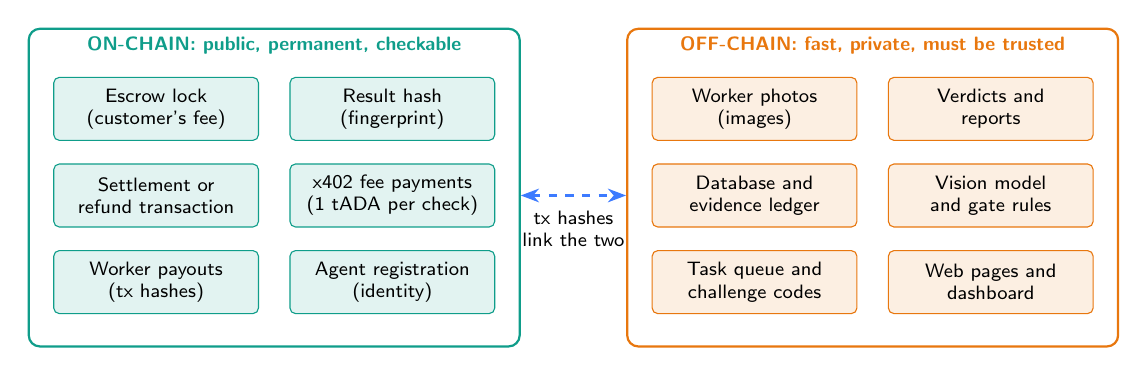
\begin{tikzpicture}[font=\sffamily\scriptsize,
    on/.style={draw=cTeal,fill=cTeal!12,rounded corners=2pt,align=center,minimum width=2.6cm,minimum height=8mm},
    off/.style={draw=cOrange,fill=cOrange!12,rounded corners=2pt,align=center,minimum width=2.6cm,minimum height=8mm}]
  \foreach \t [count=\i from 0] in {Escrow lock\\(customer's fee),Settlement or\\refund transaction,Worker payouts\\(tx hashes)}
    \node[on] at (0,-\i*1.1) {\t};
  \foreach \t [count=\i from 0] in {Result hash\\(fingerprint),x402 fee payments\\(1 tADA per check),Agent registration\\(identity)}
    \node[on] at (3,-\i*1.1) {\t};
  \foreach \t [count=\i from 0] in {Worker photos\\(images),Database and\\evidence ledger,Task queue and\\challenge codes}
    \node[off] at (7.6,-\i*1.1) {\t};
  \foreach \t [count=\i from 0] in {Verdicts and\\reports,Vision model\\and gate rules,Web pages and\\dashboard}
    \node[off] at (10.6,-\i*1.1) {\t};
  \begin{scope}[on background layer]
    \node[draw=cTeal,thick,rounded corners=4pt,fit={(-1.5,0.9) (4.5,-2.9)},label={[text=cTeal,font=\sffamily\bfseries\scriptsize,anchor=north]north:ON-CHAIN: public, permanent, checkable}] (L) {};
    \node[draw=cOrange,thick,rounded corners=4pt,fit={(6.1,0.9) (12.1,-2.9)},label={[text=cOrange,font=\sffamily\bfseries\scriptsize,anchor=north]north:OFF-CHAIN: fast, private, must be trusted}] (R) {};
  \end{scope}
  \draw[<->,dashed,thick,cSky] (L.east|-0,-1.1) -- node[below=2pt,align=center,text=black] {tx hashes\\link the two} (R.west|-0,-1.1);
\end{tikzpicture}}
\end{center}

\subsection{Properties side by side}
\begin{center}
\small
\begin{tabularx}{\textwidth}{@{}l X X@{}}
\toprule
 & \textbf{On-chain} & \textbf{Off-chain}\\
\midrule
Who can read it & Everyone (public chain) & Only those with access\\
Can it be changed later & \no\ (append-only history) & \yes\ (the owner can edit or delete)\\
Can a third party verify it without trusting us & \yes & \no\ (they must trust the operator)\\
Cost & Network fee per transaction (about 0.17~ADA on preprod) & Almost free\\
Speed & Seconds to minutes until confirmed; escrow flows take an hour or more & Milliseconds\\
Privacy & Poor: never put personal data or photos on a public chain & Good, if we protect it\\
Storage size & Tiny and expensive & Large and cheap\\
\bottomrule
\end{tabularx}
\end{center}

\begin{analogybox}{a courtroom ledger versus your notebook}
The chain is the official court ledger in a public hall. Everything written there is permanent, anyone may inspect it, but each entry costs a stamp fee and takes a while. Your notebook (off-chain) is fast, free and private, but nobody else can be sure you did not rewrite a page. Sensible people keep their drafts in the notebook and enter only the important, disputable facts in the ledger.
\end{analogybox}

\section{Hash commitments: proving without publishing}
Often we want the permanence of the chain but not the size or privacy cost of the data. The standard tool is a \term{hash}: a function that turns any data into a short fixed-length fingerprint (for example 64 hexadecimal characters for SHA-256). Three properties matter:
\begin{itemize}
  \item the same input always gives the same hash;
  \item changing even one character of the input changes the hash completely;
  \item you cannot recover the input from the hash.
\end{itemize}
A \term{hash commitment} puts only the hash on-chain. Later, anybody who holds the original data can recompute the hash and compare. If they match, the data is exactly what was committed at that time.

\begin{center}
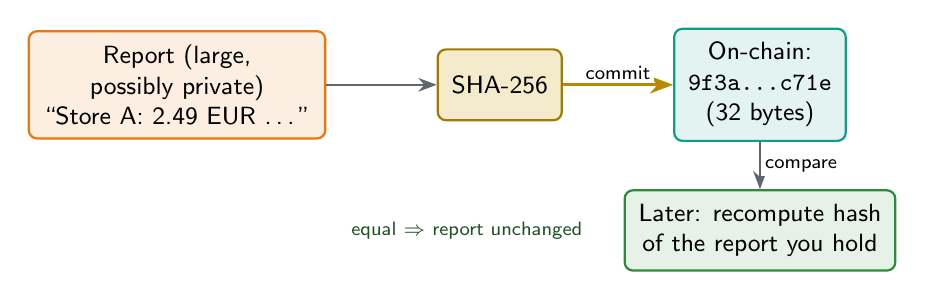
\begin{tikzpicture}[font=\sffamily\scriptsize,node distance=6mm and 14mm]
  \node[box,fill=cOrange!12,draw=cOrange] (r) {Report (large,\\possibly private)\\``Store A: 2.49 EUR \ldots''};
  \node[box,fill=cGold!20,draw=cGold!80!black,right=of r] (h) {SHA-256};
  \node[chain,right=of h] (c) {On-chain:\\\texttt{9f3a...c71e}\\(32 bytes)};
  \node[good,below=of c] (l) {Later: recompute hash\\of the report you hold};
  \draw[flow] (r) -- (h);
  \draw[pay] (h) -- node[lbl,above] {commit} (c);
  \draw[flow] (c) -- node[lbl,right] {compare} (l);
  \node[left=4mm of l,text=cGreen!60!black] {equal $\Rightarrow$ report unchanged};
\end{tikzpicture}
\end{center}

\begin{examplebox}{a tampered report}
Shelfie delivers a report saying ``lowest price 2.49 EUR'' and commits its hash \code{9f3a\ldots} on-chain. Next week someone alters the file to say ``2.19 EUR''. The hash of the altered file is completely different, so the comparison with the on-chain value fails and the change is exposed. The report itself never had to be public.
\end{examplebox}

\begin{shelfiebox}{where hashes appear}
Our evidence ledger is a hash-chained, append-only file: each line stores the hash of the previous line, so editing history breaks the chain. Photos are identified by their SHA-256, which also catches the same photo being uploaded twice. In the Masumi flow the seller submits a \emph{result hash} to the escrow; the full result text stays off-chain. Chapter~4 covers the Masumi side.
\end{shelfiebox}

\section{Escrow from zero}
\subsection{The problem}
Customer and provider do not trust each other. If the customer pays first, the provider may disappear. If the provider works first, the customer may refuse to pay. An \term{escrow} solves this with a neutral holder: the customer deposits the money with the holder, the provider does the work, and the holder pays out only when the agreed condition is met.

\begin{analogybox}{notary and Treuhand}
When you buy a flat in Germany, the buyer does not hand the price to the seller directly. A \emph{Notar} (or a \emph{Treuhandkonto}, a trust account) holds the money until the ownership is registered. Escrow is that, only the notary is replaced by a small program on the blockchain.
\end{analogybox}

\subsection{Smart-contract escrow}
A \term{smart contract} is a program stored on the chain that holds funds and releases them only under coded rules, which nobody (not even the provider) can override. Such an escrow has a small state machine with deadlines (``timeouts''):

\begin{center}
\resizebox{\textwidth}{!}{%
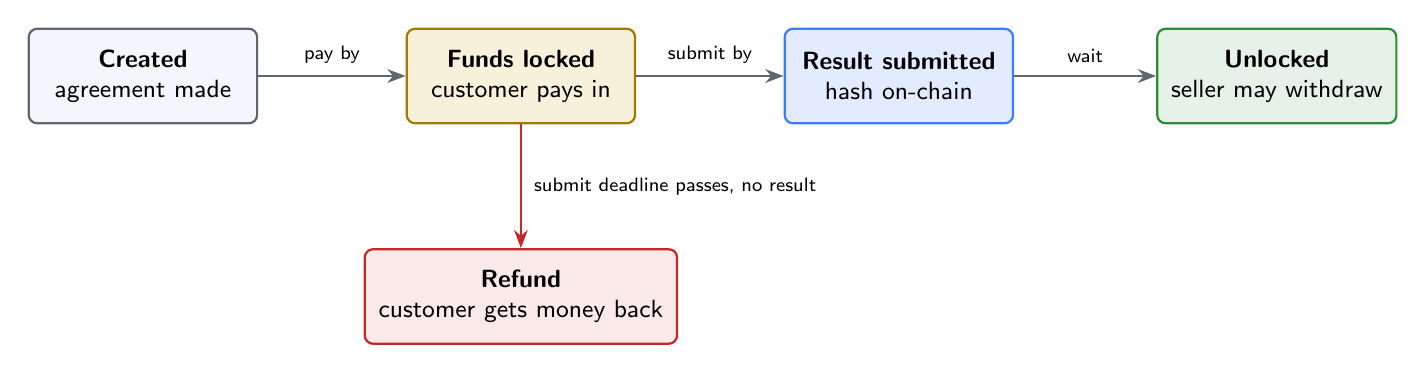
\begin{tikzpicture}[x=1cm,y=1cm,st/.style={box,minimum width=2.9cm,minimum height=1.2cm}]
  \node[st,fill=cLight,draw=cGrey] (a) at (0,0) {\textbf{Created}\\agreement made};
  \node[st,fill=cGold!15,draw=cGold!80!black] (b) at (4.8,0) {\textbf{Funds locked}\\customer pays in};
  \node[st,fill=cSky!15,draw=cSky] (c) at (9.6,0) {\textbf{Result submitted}\\hash on-chain};
  \node[st,fill=cGreen!12,draw=cGreen] (d) at (14.4,0) {\textbf{Unlocked}\\seller may withdraw};
  \node[st,fill=cRed!10,draw=cRed] (e) at (4.8,-2.8) {\textbf{Refund}\\customer gets money back};
  \draw[flow] (a)--(b) node[lbl,midway,above=1mm,fill=none] {pay by};
  \draw[flow] (b)--(c) node[lbl,midway,above=1mm,fill=none] {submit by};
  \draw[flow] (c)--(d) node[lbl,midway,above=1mm,fill=none] {wait};
  \draw[flow,draw=cRed] (b)--(e) node[lbl,midway,right=1mm,fill=none] {submit deadline passes, no result};
\end{tikzpicture}}
\end{center}

Three deadlines drive everything:
\begin{enumerate}
  \item \textbf{Pay-by:} until when the customer must lock the funds.
  \item \textbf{Submit-by:} until when the provider must submit a result (its hash).
  \item \textbf{Unlock:} after a waiting period following the submission, the provider can withdraw the money. The waiting period gives the customer time to complain.
\end{enumerate}
If the provider misses the submit deadline, the customer can get a \term{refund}. That refund path is what makes the customer comfortable paying before delivery.

\subsection{The timing facts for Masumi (from the team's runbook)}
These are estimates from the research notes (\code{investigacion/cardano/masumi-runbook.md}) and must be confirmed with the Masumi mentors on Friday.

\begin{center}
\small
\begin{tabularx}{\textwidth}{@{}l X@{}}
\toprule
\textbf{Fact} & \textbf{Value}\\
\midrule
A full paid cycle (lock, result, settlement) & at least about 60 minutes\\
Provider payout eligible & about $+46$ min counted from the start of the job: unlock at $+36$ plus about 10 min queue (runbook inference; needs a result hash)\\
Refund eligible if no result hash & about $+30$ min from the start: submit deadline at $+20$ plus about 10 min (estimate; buyer automation to verify)\\
Official docs mention longer defaults & Up to about 12 hours in some documentation; the hackathon setup is shorter. Verify.\\
\bottomrule
\end{tabularx}
\end{center}

\begin{center}
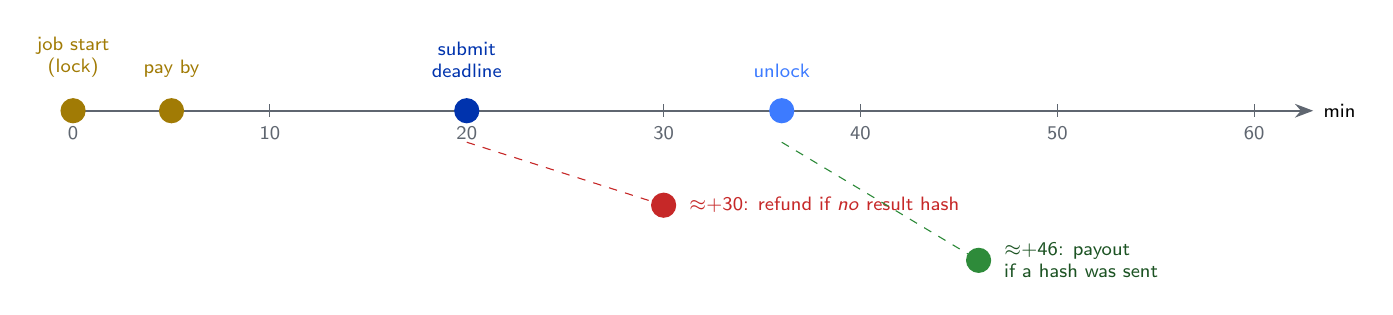
\begin{tikzpicture}[x=0.25cm,y=1cm,font=\sffamily\scriptsize]
  \draw[thick,->,draw=cGrey] (0,0) -- (63,0) node[right] {min};
  \foreach \x in {0,10,20,30,40,50,60}{\draw[cGrey] (\x,0.08)--(\x,-0.08); \node[below,text=cGrey] at (\x,-0.08) {\x};}
  \foreach \x/\t/\c in {0/job start\\(lock)/cGold!80!black,5/pay by/cGold!80!black,20/submit\\deadline/cBlue,36/unlock/cSky}{
    \fill[\c] (\x,0) circle (1.6mm); \node[above=3mm,text=\c,align=center] at (\x,0) {\t};}
  \fill[cRed] (30,-1.2) circle (1.6mm); \node[right=2mm,text=cRed,align=left] at (30,-1.2) {$\approx$+30: refund if \emph{no} result hash};
  \draw[cRed,dashed] (20,-0.4) -- (30,-1.2);
  \fill[cGreen] (46,-1.9) circle (1.6mm); \node[right=2mm,text=cGreen!60!black,align=left] at (46,-1.9) {$\approx$+46: payout\\if a hash was sent};
  \draw[cGreen,dashed] (36,-0.4) -- (46,-1.9);
\end{tikzpicture}
\end{center}

\begin{warningbox}{any result hash pays the seller}
The escrow cannot judge quality. If the provider submits \emph{any} result hash, even for a report saying ``failed'', the seller is paid after the unlock period. Marking the Sokosumi task as failed does \emph{not} refund. To trigger the refund, the provider must \textbf{withhold} the result: submit no hash at all and let the deadline pass.
\end{warningbox}

\begin{shelfiebox}{the K-of-N rule and withholding}
A brand hires Shelfie to check a product in $N$ stores and requires at least $K$ verified photos. The engine decides. If at least $K$ pass, the shell submits the report hash and the seller is paid. If fewer than $K$ pass, the shell submits \emph{nothing} (ADR-11), so the brand's money flows back automatically after the timeout. Workers whose individual photos passed are still paid (ADR-09), which Shelfie bears as a stated cost.
\end{shelfiebox}

\begin{center}
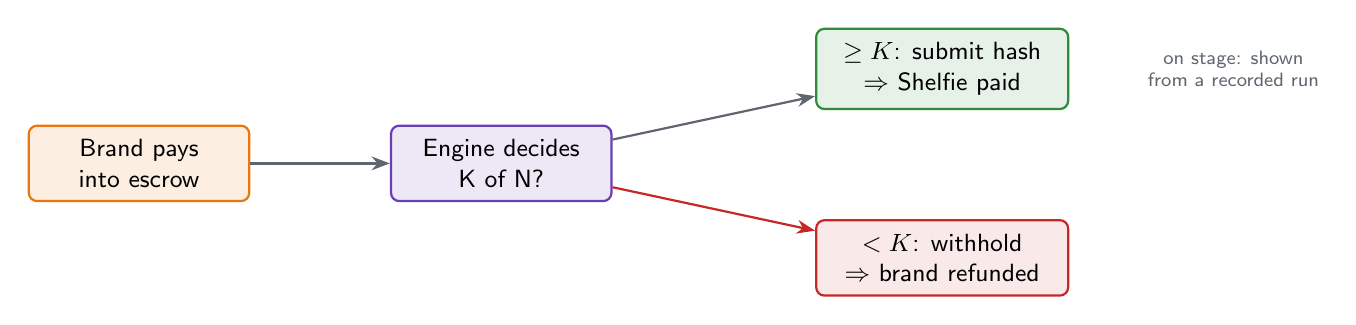
\begin{tikzpicture}[x=1cm,y=1cm]
  \node[human,minimum width=2.8cm] (b) at (0,0) {Brand pays\\into escrow};
  \node[agent,minimum width=2.8cm] (e) at (4.6,0) {Engine decides\\K of N?};
  \node[good,minimum width=3.2cm] (p) at (10.2,1.2) {$\ge K$: submit hash\\$\Rightarrow$ Shelfie paid};
  \node[bad,minimum width=3.2cm] (r) at (10.2,-1.2) {$<K$: withhold\\$\Rightarrow$ brand refunded};
  \draw[flow] (b)--(e); \draw[flow] (e)--(p); \draw[flow,draw=cRed] (e)--(r);
  \node[font=\sffamily\scriptsize,text=cGrey,align=center] at (13.9,1.2) {on stage: shown\\from a recorded run};
\end{tikzpicture}
\end{center}
This is why ADR-05 starts the first paid cycle on Friday afternoon, runs the failure/refund job on Friday night, and completes the last paid cycle by 13:00 on Saturday: the live stage can only show the verify and payout legs; settlement and refund are shown from recordings with explorer links, labelled as such.

\section{Oracles and the oracle problem}
A blockchain only knows what is inside it. It cannot look at a shelf, read a price on a website, or check the weather. An \term{oracle} is a bridge that brings real-world facts onto the chain. The \term{oracle problem} is that this bridge is a trust problem: if the chain accepts a fact, someone had to report it, and that someone could be wrong or lying. Decentralisation of the ledger does not decentralise the truth about the outside world.

\begin{center}
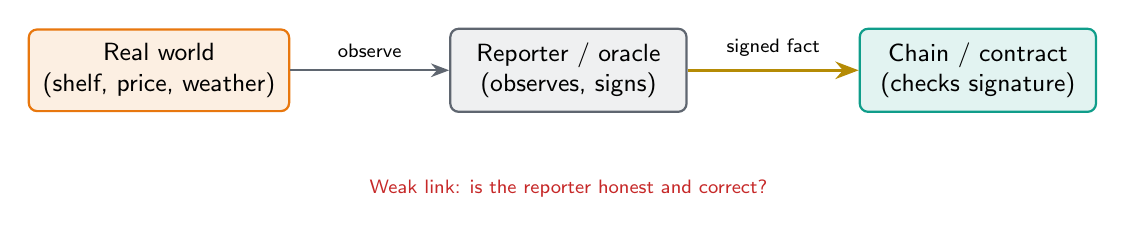
\begin{tikzpicture}[x=1cm,y=1cm]
  \node[human,minimum width=3cm] (w) at (0,0) {Real world\\(shelf, price, weather)};
  \node[service,minimum width=3cm] (o) at (5.2,0) {Reporter / oracle\\(observes, signs)};
  \node[chain,minimum width=3cm] (c) at (10.4,0) {Chain / contract\\(checks signature)};
  \draw[flow] (w)--(o) node[lbl,midway,above=1mm,fill=none] {observe};
  \draw[pay] (o)--(c) node[lbl,midway,above=1mm,fill=none] {signed fact};
  \node[font=\sffamily\scriptsize,text=cRed,align=center] at (5.2,-1.5) {Weak link: is the reporter honest and correct?};
\end{tikzpicture}
\end{center}

\begin{conceptbox}{approaches to the problem}
(1) Trust one named reporter and make it accountable (reputation, deposits, contracts). (2) Use signed data from the original source, so the contract verifies the signer, the request and the freshness instead of trusting a middleman. (3) Combine several independent reporters. None removes trust completely; they only make it explicit and checkable.
\end{conceptbox}

\begin{examplebox}{the API3 hackathon track}
This hackathon has another partner track, \emph{API3 -- Any API in your contract}. There the central feature must depend on authenticated data from AirnodeHub: a user brings the signed response on-chain and the contract verifies the expected signer, the intended request and the freshness before acting. Judges run a ``tamper test'' with one valid and four rejected responses (edited value, too old, wrong request, wrong key's signature). That is the oracle problem solved with signed data. We do not depend on it; entering API3 as a secondary track is undecided (\code{diseno/decisions.md}).
\end{examplebox}

\begin{shelfiebox}{Shelfie is a small oracle}
The fact ``this product was on this shelf at this time'' is a real-world fact that the chain cannot see. Our verifier is the reporter. We do not claim to remove the trust; we make it small and inspectable: a random single-use challenge code in the photo shows freshness (not location, an honest limit stated in ADR-12), deterministic gate rules decide instead of a model's opinion, and an append-only evidence ledger plus payment hashes make each decision auditable.
\end{shelfiebox}

\section{Trust model: who must trust whom?}
\begin{center}
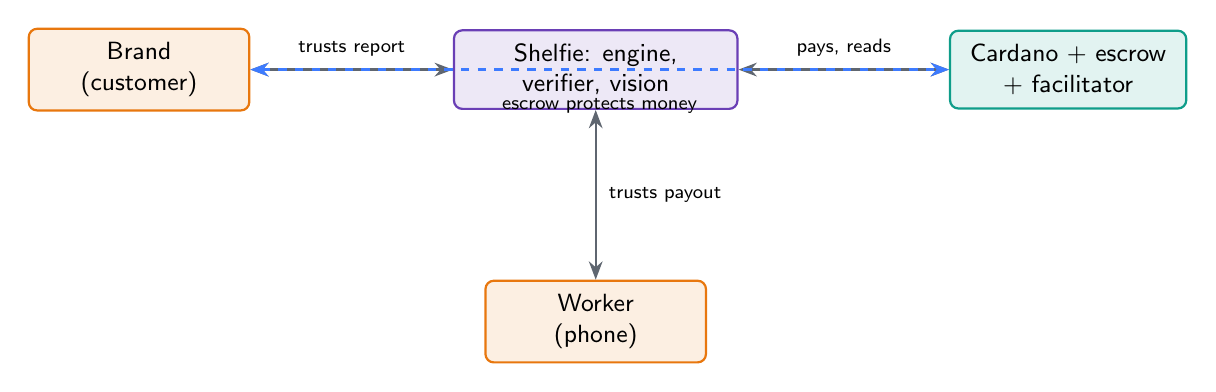
\begin{tikzpicture}[x=1cm,y=1cm]
  \node[human,minimum width=2.8cm] (br) at (0,0) {Brand\\(customer)};
  \node[agent,minimum width=3.6cm] (sh) at (5.8,0) {Shelfie: engine,\\verifier, vision};
  \node[chain,minimum width=3.0cm] (ch) at (11.8,0) {Cardano + escrow\\+ facilitator};
  \node[human,minimum width=2.8cm] (wk) at (5.8,-3.2) {Worker\\(phone)};
  \draw[flow,<->] (br)--(sh) node[lbl,midway,above=1mm,fill=none] {trusts report};
  \draw[flow,<->] (sh)--(ch) node[lbl,midway,above=1mm,fill=none] {pays, reads};
  \draw[flow,<->] (wk)--(sh) node[lbl,midway,right=1mm,fill=none] {trusts payout};
  \draw[data,<->] (br) -- (ch) node[lbl,pos=0.5,below=3mm,fill=none] {escrow protects money};
\end{tikzpicture}
\end{center}

\begin{center}
\small
\begin{tabularx}{\textwidth}{@{}l X X X@{}}
\toprule
\textbf{Party} & \textbf{Must trust} & \textbf{Why / protection} & \textbf{Residual risk}\\
\midrule
Brand (customer) & The verifier and engine to judge photos honestly; the chain & Escrow refunds if no result; rules are deterministic; ledger and hashes are auditable & We could still be wrong or biased; freshness is proven, location is not\\
Worker & The engine to pay verified photos & Payout appears as a tx hash on Cardanoscan; visible and permanent & A failed payout needs the queue and reconcile logic\\
Shelfie engine & The verifier's verdicts and the facilitator & Verifier is ours; payments are checkable on-chain & Vision model errors; provider outage (a flagged demo override exists)\\
Verifier seller & The facilitator to settle correctly & Facilitator is non-custodial; hashes can be checked on-chain & If down, no paid checks (fallback: local facilitator)\\
Everyone & Cardano preprod itself & Public ledger, many nodes & It is a test network; tADA has no value, and resets or outages are possible\\
\bottomrule
\end{tabularx}
\end{center}


\section{What can go wrong: failure scenarios}
Understanding the trust model is easiest by walking through bad days. The table lists what happens, what protects us, and what we still have to build or check.
\begin{center}
\small
\begin{tabularx}{\textwidth}{@{}X X X@{}}
\toprule
\textbf{Scenario} & \textbf{What the design does} & \textbf{Status / to verify}\\
\midrule
Brand pays but Shelfie never delivers & No result hash is submitted, so the escrow refunds the brand after the timeout & Timing is an estimate; verify with Masumi mentors\\
Job fails K-of-N but the shell submits a ``failed'' text & Seller is paid anyway (any hash pays) & Prevented by design: withhold the result\\
Verifier is paid but the vision model is down & Error returned before settlement where possible; engine retries with the same idempotency key & Exact order in the template to be verified Friday\\
Payout transaction times out & Queue marks it unknown, searches the chain for the metadata tag, pays again only if absent & Metadata support in the SDK is unverified\\
Worker uploads an old photo & Challenge code and timing checks reject it; the check still costs 1~tADA & Honest limit: freshness, not location\\
Hosted facilitator unreachable & Seller answers 500; fall back to a local facilitator (\code{npm run facilitator}) & Test before the demo\\
Preprod network is slow & Stage shows recorded settlement; the live part is verify and payout & Decided in ADR-05\\
\bottomrule
\end{tabularx}
\end{center}

\subsection{Finality: when is ``on-chain'' really final?}
A transaction is not final the instant it is submitted. It is first accepted into a block and then becomes harder and harder to reverse as more blocks follow. The x402 default is one confirmation before the facilitator reports success; a faster mode with zero confirmations exists and hosted facilitators accept it, at the price of a small risk that the payment does not end up in the chain. For the demo this explains why one verify payment takes 20 to 60 seconds, and why a ``timed out'' call must be checked on the explorer before retrying.

\begin{analogybox}{a cheque versus cash in hand}
Submitting a transaction is like handing over a cheque; the confirmation is the bank clearing it. You may deliver the goods when the bank says it is cleared, or earlier if you accept a little risk. Escrow adds a third option: the cheque is already deposited with the notary before you start work.
\end{analogybox}

\section{What is on-chain and off-chain in Shelfie}
\begin{center}
\small
\begin{tabularx}{\textwidth}{@{}l c c X@{}}
\toprule
\textbf{Item} & \textbf{On-chain} & \textbf{Off-chain} & \textbf{Notes}\\
\midrule
Brand's fee in escrow (lock) & \yes & & Masumi escrow; tx hash\\
Settlement or refund & \yes & & After the timing window; shown from a recording on stage\\
Result hash & \yes & & Fingerprint only; report text is off-chain\\
x402 verify fee, 1 tADA & \yes & & One transaction per check, pass or fail\\
Worker payout, 3 tADA (planned) & \yes & & Plain transfer, tx hash on Cardanoscan; metadata tag \code{shelfie:<payoutId>} planned (verify Friday)\\
Worker photos & & \yes & Large, personal; only SHA-256 hashes are used\\
Verdicts, gate results, reports & & \yes & Kept in the engine and ledger\\
Task queue, claims, challenge codes & & \yes & In-memory state plus event log on disk\\
Evidence ledger (\code{evidence.jsonl}) & & \yes & Hash-chained and append-only; links to tx hashes\\
Vision model and rules & & \yes & Provider is configuration (ADR-07)\\
Dashboard and worker page & & \yes & Served through an HTTPS tunnel\\
\bottomrule
\end{tabularx}
\end{center}

\begin{center}
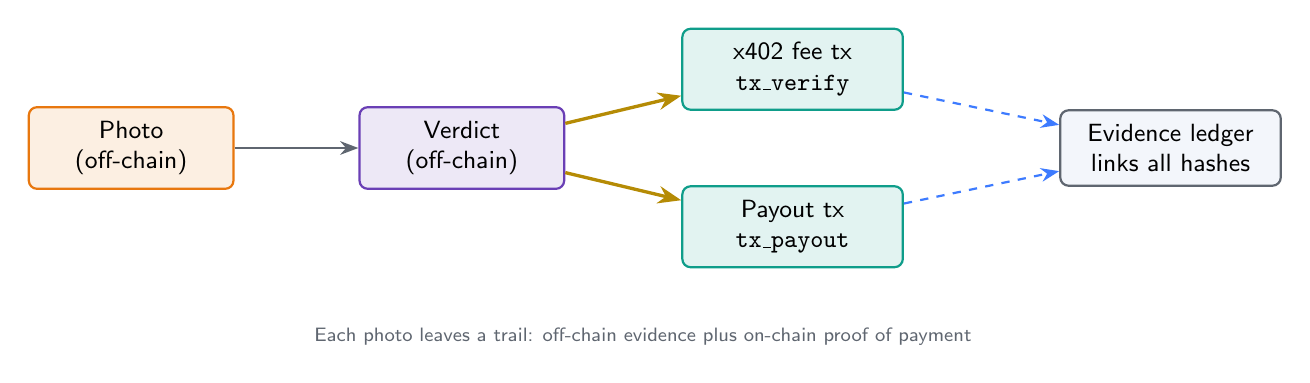
\begin{tikzpicture}[x=1cm,y=1cm]
  \node[human,minimum width=2.6cm] (ph) at (0,0) {Photo\\(off-chain)};
  \node[agent,minimum width=2.6cm] (vd) at (4.2,0) {Verdict\\(off-chain)};
  \node[chain,minimum width=2.8cm] (fee) at (8.4,1.0) {x402 fee tx\\\code{tx\_verify}};
  \node[chain,minimum width=2.8cm] (pay) at (8.4,-1.0) {Payout tx\\\code{tx\_payout}};
  \node[box,fill=cLight,draw=cGrey,minimum width=2.8cm] (led) at (13.2,0) {Evidence ledger\\links all hashes};
  \draw[flow] (ph)--(vd); \draw[pay] (vd)--(fee); \draw[pay] (vd)--(pay);
  \draw[data] (fee)--(led); \draw[data] (pay)--(led);
  \node[font=\sffamily\scriptsize,text=cGrey] at (6.5,-2.4) {Each photo leaves a trail: off-chain evidence plus on-chain proof of payment};
\end{tikzpicture}
\end{center}

\begin{warningbox}{do not oversell ``on-chain''}
Do not tell judges that the verdicts are on a blockchain. The honest claim: money movements and the escrow are on-chain and independently checkable; the judgement itself is off-chain and is made auditable through rules, a hash-chained ledger and payment hashes. Also say clearly that settlement and refund on stage are from earlier recorded runs.
\end{warningbox}

\begin{keypoints}
\begin{itemize}
\item On-chain = public, permanent and checkable but costly and slow; off-chain = fast, private and cheap but requires trust in the operator.
\item A hash commitment puts a fingerprint on-chain and keeps the data elsewhere; any later change is detectable.
\item Escrow holds money until a condition is met; with deadlines (pay-by, submit-by, unlock) and a refund path it protects the customer without a human notary.
\item Masumi timing (estimates): paid cycle at least 60 min, payout eligible at about $+46$ min and refund at about $+30$ min, both counted from the start of the job.
\item Submitting any result hash pays the seller, so a failed job must withhold the result to trigger a refund.
\item An oracle brings real-world facts on-chain, but trust moves rather than disappears. Shelfie is a small oracle for shelf facts and makes its trust explicit.
\item Shelfie on-chain: escrow, x402 fees, payouts. Off-chain: photos, verdicts, database, ledger, vision model.
\end{itemize}
\end{keypoints}

\begin{quizbox}
\begin{enumerate}
  \item Why should photos not be stored on a public blockchain?
  \item What does a hash commitment prove, and what does it not reveal?
  \item List the three deadlines of a timeout-based escrow and say what each protects.
  \item A job fails the K-of-N rule. Which action leads to a refund and which action would wrongly pay the seller?
  \item What is the oracle problem, and how is Shelfie an example of it?
  \item Name two things Shelfie records on-chain and two that stay off-chain.
\end{enumerate}
{\footnotesize\color{cGrey}\textbf{Answers.} (1) Public, permanent, size-limited and expensive; privacy would be lost. (2) That data existing now matches the committed fingerprint, so later changes are detected; it does not reveal the data. (3) Pay-by (customer must fund), submit-by (provider must deliver), unlock (waiting period before the provider withdraws; time to complain). (4) Withholding the result triggers the refund; submitting any hash, even ``failed'', pays the seller. (5) The chain cannot see the real world, so someone must report facts and be trusted; Shelfie reports ``product was on the shelf''. (6) On-chain: escrow, x402 fee, payouts; off-chain: photos, verdicts, ledger, vision model.\par}
\end{quizbox}


\part{Our idea: Shelfie}
\chapter{Shelfie: the idea}

\section*{Why this matters for us}
The first five chapters gave you the tools: blockchain, Cardano, HTTP~402 and x402, agents with Masumi and Sokosumi, and the difference between on-chain and off-chain. This chapter is the first time we put them to work on \emph{our} product. If you can explain Shelfie in two minutes to a stranger, to a judge, and to a friend who has never heard of blockchains, you have understood the project. Everything in chapters 7 to 9 (engine, verifier, hackathon day) builds on the story told here.

\section{The problem: nobody can see the shelf}

\subsection{Retail execution in plain words}
A small drinks brand sells its bottles to a supermarket chain. The contract is signed, the pallets are delivered to the warehouse. But does the bottle actually stand on the shelf in store number 7 in Munich? At which price? Is the shelf tag correct, or is the product hidden behind a competitor's? The work of making sure that a product arrives on the shelf as agreed is called \term{retail execution}. The people who do it for brands are called field-sales or merchandising staff, and many brands hire external companies for it.

Three words that you will meet again:
\begin{itemize}
  \item \term{Retail execution}: making sure the agreed product, price and placement really appear in the store.
  \item \term{Field marketing} (or merchandising): sending people into stores to check, restock or promote products.
  \item \term{Mystery shopping}: a person visits a store, pretends to be a normal customer and reports what they see.
\end{itemize}

\begin{analogybox}{The restaurant delivery photo}
You order food and the app says ``delivered''. You would like a photo of the parcel at your door, taken \emph{now}, not last week. A brand ordering a shelf check has the same wish: ``show me the shelf as it is today''. Shelfie sells exactly that photo, and pays the photographer only if the photo is real.
\end{analogybox}

\subsection{What the options cost today (marked as inference)}
Today a brand has three choices, none of them good:

\begin{center}
\small
\begin{tabularx}{\textwidth}{@{}p{3.4cm}XX@{}}
\toprule
\textbf{Option} & \textbf{Problem} & \textbf{Status of the claim}\\
\midrule
Drive around yourself & An afternoon for 10 stores, and it does not scale. & Plain logic.\\
Field-marketing agency or mystery-shopping panel & Booked days ahead; paid per visit whether or not the photo is usable. & \emph{Inference.} Price per visit and lead time still need two public sources.\\
Trust the chain's own sales data & It tells you what was sold, not what stands on the shelf. & Plain logic.\\
\bottomrule
\end{tabularx}
\end{center}

\begin{warningbox}{Do not state numbers we have not sourced}
The team's notes carry the placeholder \texttt{[SOURCE NEEDED]} for the price of an agency visit, the typical lead time and the share of sales lost to missing products. In the pitch we only say ``booked days ahead, paid per visit'' unless we find sources. A made-up number can sink credibility with judges.
\end{warningbox}

\section{Our fictional customer: Katharina Brandl}
Every pitch needs one concrete person. Ours is \textbf{fictional} and we say so whenever asked:

\begin{shelfiebox}{Persona (invented for the story)}
\textbf{Katharina Brandl}, field-sales manager at \textbf{Isarquell}, a small Bavarian craft-lemonade brand (invented, no real company). There are four people in sales. Last month Katharina sold a new 0.33~l bottle to a regional supermarket chain. Today she needs to know: \emph{is it on the shelf in 10 Munich stores, and at which price, right now?}
\end{shelfiebox}

Why a persona at all? The Cardano track judges explicitly want to see a \emph{clear customer and journey}. A name, a job and a concrete question turn an abstract protocol into a story that people remember.

\subsection{The job: ``check product X in N stores''}
Katharina does not want to learn about blockchains. She wants one sentence to work:

\begin{center}
\fbox{\parbox{0.88\textwidth}{\centering\sffamily\textbf{``Check Isarquell 0.33~l in 10 Munich stores.''}}}
\end{center}

She posts this job on Sokosumi (the marketplace from Chapter~4) to the \emph{Shelfie lead agent}. The fee for the job is locked in Masumi escrow (Chapter~4). From her side that is all. What happens next is Shelfie's work, and it is the subject of the rest of this guide.

\section{The three payment gates}
Here is the heart of the product. Money moves in three places, and each place has a rule that must be satisfied first. The team's pitch calls them the \term{three payment gates}:

\begin{enumerate}
  \item \textbf{Photo gate: pays the human.} The verifier agent checks one photo. If it passes, the person who took it receives a payout on Cardano preprod right away. If it fails, nothing is paid and the task reopens.
  \item \textbf{Job gate: settles the escrow.} When all stores are done or the time window closes, the engine counts passed stores. If at least $K$ of $N$ passed, the report is delivered and the escrow settles.
  \item \textbf{Fallback: refund.} If fewer than $K$ passed, the report is withheld and the brand is refunded automatically.
\end{enumerate}

\begin{warningbox}{Two kinds of ``gates''}
Do not confuse the three \emph{payment gates} above with the seven \emph{verifier checks} G1 to G7 (Chapter~8). The photo gate is \emph{made of} G1 to G7. The pitch says ``three gates''; the verifier spec says ``G1 to G7''.
\end{warningbox}

\begin{figure}[htbp]
\centering
\resizebox{\textwidth}{!}{%
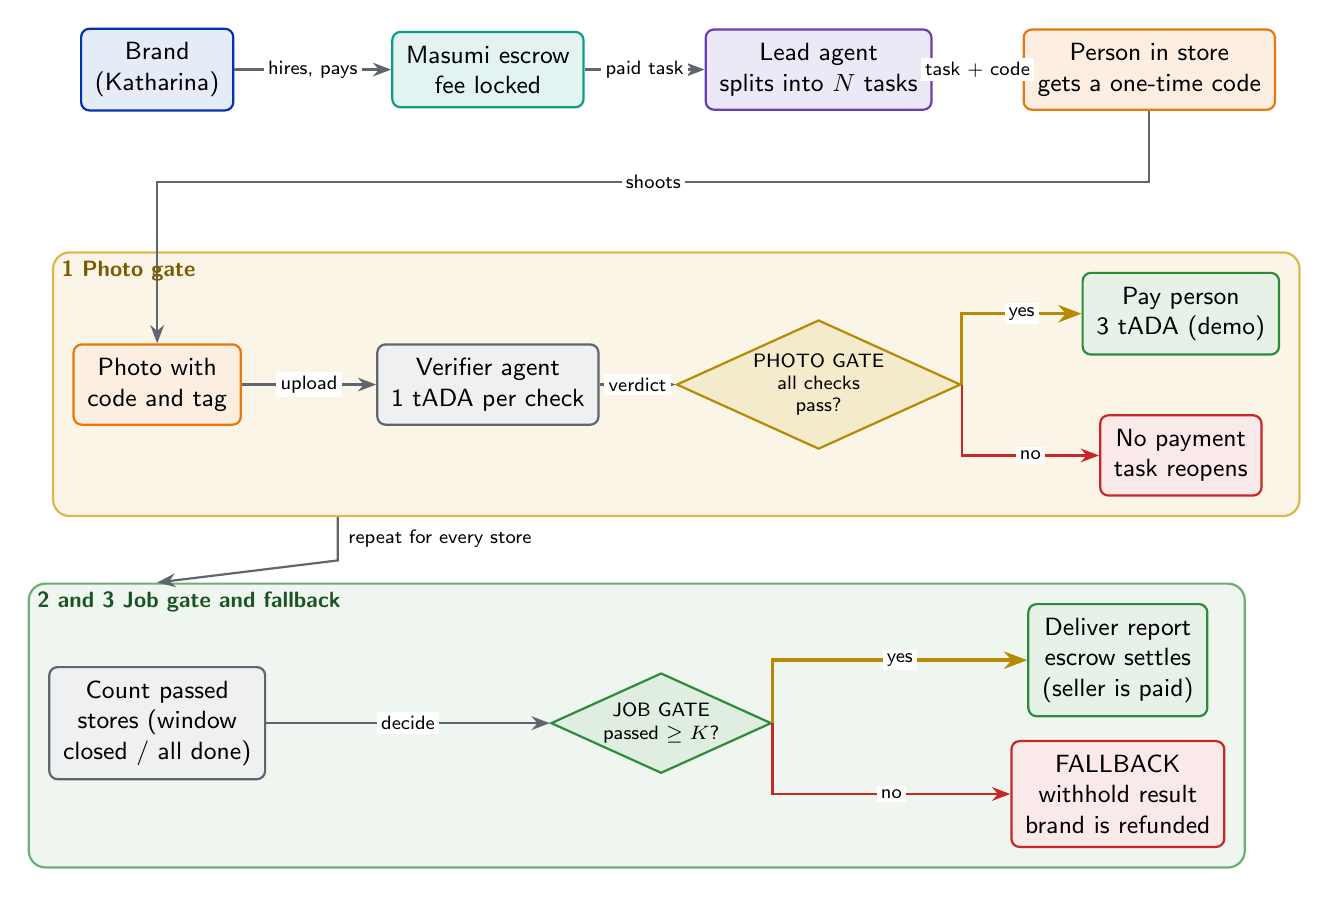
\begin{tikzpicture}[node distance=6mm,
  band/.style={rounded corners=6pt,thick,inner sep=7pt},
  dec/.style={diamond,aspect=2.2,draw,thick,align=center,font=\sffamily\scriptsize,inner sep=1pt}]
% Row 0: hiring
\node[actor] (brand) at (0,0) {Brand\\(Katharina)};
\node[chain] (esc) at (4.2,0) {Masumi escrow\\fee locked};
\node[agent] (lead) at (8.4,0) {Lead agent\\splits into $N$ tasks};
\node[human] (wk) at (12.6,0) {Person in store\\gets a one-time code};
\draw[flow] (brand) -- node[lbl]{hires, pays} (esc);
\draw[flow] (esc) -- node[lbl]{paid task} (lead);
\draw[flow] (lead) -- node[lbl]{task + code} (wk);
% Band 1
\node[human] (ph) at (0,-4) {Photo with\\code and tag};
\node[service] (ver) at (4.2,-4) {Verifier agent\\1 tADA per check};
\node[dec,fill=cGold!20,draw=cGold!90!black] (g1) at (8.4,-4) {PHOTO GATE\\all checks\\pass?};
\node[good] (pay) at (13,-3.1) {Pay person\\3 tADA (demo)};
\node[bad] (no) at (13,-4.9) {No payment\\task reopens};
\draw[flow] (wk.south) -- ++(0,-0.9) -| node[lbl,pos=0.25]{shoots} (ph.north);
\draw[flow] (ph) -- node[lbl]{upload} (ver);
\draw[flow] (ver) -- node[lbl]{verdict} (g1);
\draw[pay] (g1.east) |- node[lbl,pos=0.75]{yes} (pay.west);
\draw[flow,draw=cRed] (g1.east) |- node[lbl,pos=0.75]{no} (no.west);
\begin{scope}[on background layer]
\node[band,fill=cGold!10,draw=cGold!70,fit=(ph)(ver)(g1)(pay)(no)] (b1) {};
\end{scope}
\node[font=\sffamily\bfseries\footnotesize,text=cGold!60!black,anchor=north west] at (b1.north west) {1  Photo gate};
% Band 2
\node[service] (cnt) at (0,-8.3) {Count passed\\stores (window\\closed / all done)};
\node[dec,fill=cGreen!15,draw=cGreen] (g2) at (6.4,-8.3) {JOB GATE\\passed $\ge K$?};
\node[good] (del) at (12.2,-7.5) {Deliver report\\escrow settles\\(seller is paid)};
\node[bad] (ref) at (12.2,-9.2) {FALLBACK\\withhold result\\brand is refunded};
\draw[flow] (cnt) -- node[lbl]{decide} (g2);
\draw[pay] (g2.east) |- node[lbl,pos=0.75]{yes} (del.west);
\draw[flow,draw=cRed] (g2.east) |- node[lbl,pos=0.75]{no} (ref.west);
\begin{scope}[on background layer]
\node[band,fill=cGreen!8,draw=cGreen!70,fit=(cnt)(g2)(del)(ref)] (b2) {};
\end{scope}
\node[font=\sffamily\bfseries\footnotesize,text=cGreen!60!black,anchor=north west] at (b2.north west) {2 and 3  Job gate and fallback};
\draw[flow] (b1.south) ++(-4.3,0) -- ++(0,-0.55) node[lbl,right,xshift=2pt]{repeat for every store} -- (cnt.north |- b2.north);
\end{tikzpicture}}
\caption{The three payment gates. Gate~1 pays one person per accepted photo. Gate~2 and the fallback decide the whole job: either the escrow settles or the brand gets the money back.}
\end{figure}

\subsection{K of N, with numbers}
The job gate uses a simple rule: the brand pays for the job if at least $K$ stores pass out of $N$. We call this \term{K-of-N}. The default is
\[
K = \lceil 0.6\, N \rceil
\]
where $\lceil x\rceil$ means ``round up to the next whole number''. The 0.6 comes from the design files (\code{kDefault: ceil(0.6*n)}); an earlier draft said 0.7 and was corrected.

\begin{examplebox}{Worked examples}
\begin{itemize}
  \item $N=5$: $0.6\cdot 5 = 3.0$, so $K=3$. Three good photos are enough.
  \item $N=10$: $0.6\cdot 10 = 6.0$, so $K=6$. Katharina's real job.
  \item $N=7$: $0.6\cdot 7 = 4.2$, rounded up $K=5$. Rounding up makes the rule stricter, never looser.
  \item $N=3$ (our smoke test): $0.6\cdot 3=1.8$, so $K=2$.
\end{itemize}
\end{examplebox}

\begin{figure}[htbp]
\centering
\begin{tikzpicture}[st/.style={minimum width=1.05cm,minimum height=0.95cm,draw,thick,rounded corners=2pt,font=\sffamily\small\bfseries,align=center}]
\node[font=\sffamily\small\bfseries,anchor=west] at (0,1.5) {$N=5$, $K=3$: job passes (escrow settles)};
\foreach \i/\c/\t in {0/good/\yes,1/good/\yes,2/good/\yes,3/bad/\no,4/bad/\no}
  \node[st,\c] at (\i*1.3,0.5) {\t};
\node[font=\sffamily\scriptsize,anchor=west] at (7,0.5) {3 passed $\ge$ 3 needed};
\node[font=\sffamily\small\bfseries,anchor=west] at (0,-0.7) {$N=5$, $K=3$: job fails (brand is refunded)};
\foreach \i/\c/\t in {0/good/\yes,1/good/\yes,2/bad/\no,3/bad/\no,4/bad/\no}
  \node[st,\c] at (\i*1.3,-1.7) {\t};
\node[font=\sffamily\scriptsize,anchor=west] at (7,-1.7) {2 passed $<$ 3 needed};
\node[font=\sffamily\small\bfseries,anchor=west] at (0,-2.9) {$N=10$, $K=6$: job passes};
\foreach \i/\c/\t in {0/good/\yes,1/good/\yes,2/good/\yes,3/good/\yes,4/good/\yes,5/good/\yes,6/bad/\no,7/good/\yes,8/bad/\no,9/bad/\no}
  \node[st,\c,minimum width=0.85cm] at (\i*1.05,-3.9) {\t};
\node[font=\sffamily\scriptsize,anchor=west] at (10.6,-3.9) {7 $\ge$ 6};
\end{tikzpicture}
\caption{Each square is one store. Green means the verifier accepted the photo. Whether the job passes depends only on the count of green squares.}
\end{figure}

\subsection{Who bears the cost of a failed job?}
Workers whose photo was accepted are paid immediately, even if the job later fails the K-of-N rule and the brand is refunded (decision ADR-09 in the design files). Reason: paying at verification keeps the live ``photo goes green, payout appears'' moment, and workers should not wait an hour for money. Consequence: on a failed job \emph{Shelfie} bears the cost of workers already paid. The ledger records this as \code{COST\_BORNE}, and the pitch says it openly: ``we pay workers for verified work, regardless of the brand's threshold.''

\begin{conceptbox}{Why can a failed job still produce payouts?}
The two decisions are independent. The \emph{photo gate} asks: ``is this photo true?'' The \emph{job gate} asks: ``did the brand receive enough true photos?'' A true photo deserves its payout even when the other stores failed.
\end{conceptbox}

\section{The demo moment}
Judges remember one moment, not twelve slides. Ours is designed in advance:

\begin{enumerate}
  \item One teammate stands up holding a product with a printed price tag.
  \item The worker page on the phone shows a \textbf{challenge code} such as \code{K7Q-4XM}. The phone that shoots cannot show its own screen, so the code is written on paper (or a printed card from our card pool is used) and held next to the tag.
  \item The teammate takes the photo in the page's camera. The verifier highlights price and product; the row turns \textbf{green}.
  \item A payout transaction appears on the dashboard and, a few seconds later, on Cardanoscan (the preprod explorer).
  \item Then the \textbf{cheat attempt}: an old photo of the same tag, without the right code. The verifier rejects it live: red, reason ``code missing'', no payment. The verification fee is still spent (the verifier is paid per check), and we say so.
  \item Optional: invite a judge to take a photo themselves.
\end{enumerate}

\begin{figure}[htbp]
\centering
\resizebox{\textwidth}{!}{%
\begin{tikzpicture}
\node[human,minimum width=3.3cm] (a) at (0,0) {1  Phone shows code\\\code{K7Q-4XM}};
\node[human,minimum width=3.3cm] (b) at (4.4,0) {2  Code on paper\\next to the tag};
\node[agent,minimum width=3.3cm] (c) at (8.8,0) {3  Verifier reads\\price + product};
\node[good,minimum width=3.3cm] (d) at (13.2,0) {4  GREEN\\payout tx shown};
\draw[flow] (a)--(b); \draw[flow] (b)--(c); \draw[flow] (c)--(d);
\node[bad,minimum width=3.3cm] (e) at (0,-2.2) {5  Cheat: old photo\\no valid code};
\node[bad,minimum width=3.3cm] (f) at (4.4,-2.2) {Verifier: RED\\\code{code\_missing}};
\node[service,minimum width=3.3cm] (g) at (8.8,-2.2) {No payout\\fee still spent};
\node[service,minimum width=3.3cm] (h) at (13.2,-2.2) {Dashboard shows\\both rows};
\draw[flow] (e)--(f); \draw[flow] (f)--(g); \draw[flow] (g)--(h);
\draw[data] (d.south) -- ++(0,-0.6) -| (e.north);
\end{tikzpicture}}
\caption{Live demo choreography: one honest photo, then one cheat attempt.}
\end{figure}

\begin{warningbox}{How the cheat photo gets in is still open}
Over the HTTPS tunnel the worker page uses in-app capture and cannot pick a gallery photo. How the team submits the cheat photo live (LAN fallback page, operator-only upload route, or a pre-shot file through the dashboard) is an \emph{open item} in the review report. Decide Friday, rehearse, and say which method was used.
\end{warningbox}

\section{Why it fits the judging rubric}
The Cardano track description lists what the judges want to see. The table maps each wish to a feature. The right column is our reading (inference), not an official statement.

\begin{center}
\small
\begin{tabularx}{\textwidth}{@{}p{4.1cm}X@{}}
\toprule
\textbf{Judges want} & \textbf{Shelfie answers with}\\
\midrule
Clear customer and journey & Brand manager Katharina, one concrete job, a real industry (retail execution).\\
Payment tied to the result & Three gates: verifier pass pays the human; K-of-N settles the escrow; otherwise refund.\\
Agents hire agents, or act in the real world & The lead agent hires a verifier agent (x402) \emph{and} humans in physical stores.\\
Live paid task with transaction in an explorer & A photo on stage turns green and the payout tx shows on Cardanoscan.\\
Originality & Agents as employers of people; a one-time code as the freshness proof; nothing similar seen on Sokosumi.\\
Impact and continuation & Retail audits first; later any ``proof of the real world'' task: deliveries, outages, accessibility checks.\\
\bottomrule
\end{tabularx}
\end{center}

The official requirement is modest: a working agent or service that completes at least one job or payment on Cardano \textbf{preprod}. Everything beyond it is about earning the points for the criteria above.

\section{Business model (illustrative pricing)}
\begin{warningbox}{These euro figures are illustrative}
The EUR amounts below are \emph{hypotheses for the pitch}. They are not measured and not what the demo moves. The demo uses tADA, which are test coins on preprod and have no market value. Never put a tADA amount next to a EUR amount as if they were equal.
\end{warningbox}

Target: about \textbf{EUR 5 per verified store check, charged only when it passes}. One check involves five money items. Margin per check, for the bottom of the payout range and for the top:

\begin{center}
\small
\begin{tabular}{@{}lrr@{}}
\toprule
\textbf{Item per passed check} & \textbf{Low payout} & \textbf{High payout}\\
\midrule
Price to the brand (illustrative) & 5.00 & 5.00\\
Payout to the person & $-2.50$ & $-3.00$\\
Verifier cost (model + fee, estimate) & $-0.10$ & $-0.10$\\
Network/escrow fee (about 5\%, secondary source, verify) & $-0.25$ & $-0.25$\\
\midrule
\textbf{Margin before support and disputes (EUR)} & \textbf{2.15} & \textbf{1.65}\\
\bottomrule
\end{tabular}
\end{center}

Hence the margin range of \textbf{EUR 1.65 to 2.15} that appears in the pitch. Two honesty notes: (1) verifier fees spent on \emph{rejected} photos are not in this table, because rejected photos are not billed to the brand; (2) support, disputes and legal costs are not included.

\begin{figure}[htbp]
\centering
\begin{tikzpicture}
\def\s{1.15}
\fill[cBlue!70] (0,0) rectangle (5*\s*1.0,0.9);
\node[white,font=\sffamily\small\bfseries] at (2.5*\s,0.45) {Brand pays 5.00};
\fill[cOrange!80] (0,-1.3) rectangle (2.5*\s,-0.4);
\node[font=\sffamily\scriptsize] at (1.25*\s,-0.85) {Person 2.50};
\fill[cOrange!50] (2.5*\s,-1.3) rectangle (3.0*\s,-0.4);
\node[font=\sffamily\tiny] at (2.75*\s,-0.85) {+0.50};
\fill[cPurple!60] (3.0*\s,-1.3) rectangle (3.1*\s,-0.4);
\fill[cRed!50] (3.1*\s,-1.3) rectangle (3.35*\s,-0.4);
\fill[cGreen!70] (3.35*\s,-1.3) rectangle (5.0*\s,-0.4);
\node[font=\sffamily\scriptsize] at (4.2*\s,-0.85) {margin 1.65};
\end{tikzpicture}
\caption{Where one illustrative EUR 5 goes (high-payout case). Orange: payout (2.50 solid, up to 3.00 with the lighter block); purple: verifier 0.10; red: fee 0.25; green: margin.}
\end{figure}

\subsection{Who pays and why would they switch?}
Small and mid-size consumer brands without a retail-execution team. They switch for \emph{speed} (same day), \emph{proof} (a code-bound photo with an audit trail) and \emph{pay per passed check}. We have \textbf{not validated demand with interviews}; the hackathon proves a mechanism, not a market. Next step in the roadmap: five brand interviews.

\section{Limits we admit}
Judges respect honest limits more than hidden ones. The team has agreed on this list and says it plainly:

\begin{center}
\small
\begin{tabularx}{\textwidth}{@{}p{4.2cm}X@{}}
\toprule
\textbf{Limit} & \textbf{What is true}\\
\midrule
The code proves \textbf{freshness}, not \textbf{location} & A worker could photograph the same product in a different shop. Roadmap: store-owned QR codes or geofenced tasks.\\
The gate proves ``fresh and readable'', not ``genuine'' & No claim of zero fraud; a fake made live is possible in theory. The cost of cheating should exceed the payout.\\
No identity checks, no reputation & Only claim time limits, attempt caps and a duplicate-image check exist. Workers are just a wallet address.\\
Humans need a wallet & The demo uses teammates' preprod wallets. A production onboarding is roadmap.\\
Preprod only & No mainnet, no real money. The x402 facilitator is preprod-only today.\\
Settlement is shown from earlier runs & An escrow cycle takes at least 60 minutes, so on stage we show recorded lock, settlement and refund transactions and say so.\\
Legal questions open & Is per-task pay employment? Tax? Custody? Needs a legal opinion before mainnet.\\
Demo override exists & An admin-only manual override can rescue a stage demo; it is flagged red and never used in evidence runs (Chapter~8).\\
\bottomrule
\end{tabularx}
\end{center}

\section{Alternatives we considered}
The team ran two independent brainstorming rounds with 27 ideas and weighted scoring. Both put the same concept first.

\begin{center}
\small
\begin{tabularx}{\textwidth}{@{}p{3.2cm}p{2.6cm}X@{}}
\toprule
\textbf{Idea} & \textbf{Score} & \textbf{Verdict}\\
\midrule
\textbf{Shelfie} (``Eyes on Ground'' / ``Ground Truth'') & 4.25 of 5 and 7.95 of 10 & Chosen. Real-world task, deterministic pass/fail, strong live moment.\\
ShopScout & 3.35 of 5 & Solid but generic; its ``report quality'' gate is a subjective opinion, which escrow handles badly. Its plumbing is reused by Shelfie.\\
Beh\"orde Brief Decoder & 7.65 of 10 & Safest build; \textbf{Plan B}. Same architecture with an OCR worker instead of humans.\\
Termin-Sniper / CancelBot & -- & Great business models but bot-protected portals or long latency, so mock-only demos.\\
Verified Findings & -- & Easiest, least emotional.\\
\bottomrule
\end{tabularx}
\end{center}

\begin{conceptbox}{Plan B is not a separate project}
Plan B reuses the engine from Chapter~7. If feedback or a workshop forces a change, the team swaps the \emph{domain pack} (task template, verifier rules, report template) and keeps payments, agent shell and UI. A letter is uploaded, an OCR worker extracts deadline, amount and authority, rules check plausibility, and the report explains the letter. Trigger from the risk register: by Friday 17:00 the vision verifier cannot read printed tags reliably \emph{and} the labelled override is not enough.
\end{conceptbox}

\begin{keypoints}
\begin{itemize}
  \item Shelfie sells \textbf{verified shelf checks}: a brand hires an agent, which hires people to photograph shelves; payment is tied to the photo being true.
  \item Persona: Katharina Brandl at Isarquell (\textbf{fictional}). Job: ``check product X in $N$ stores''.
  \item Three payment gates: photo gate pays the human; job gate settles the escrow at $K$ of $N$ with $K=\lceil 0.6N\rceil$; fallback refunds the brand.
  \item Demo: one honest photo turns green and shows a payout tx; one cheat photo is rejected with no payment.
  \item EUR prices are \textbf{illustrative}; margin range EUR 1.65 to 2.15; the demo uses tADA on preprod.
  \item Honest limits: the code proves freshness, not location; no identity checks; settlement shown from recorded runs.
\end{itemize}
\end{keypoints}

\begin{quizbox}
\begin{enumerate}
  \item Which of the three payment gates pays a human, and what triggers it?
  \item Compute $K$ for $N=8$. Show the rounding.
  \item A job with $N=5$, $K=3$ ends with 2 accepted photos. Who has been paid, and what happens to the brand's fee?
  \item Why do we say the pricing is ``illustrative''?
  \item Give two limits of the freshness code that we admit openly.
  \item What is Plan B and what does it reuse?
\end{enumerate}
{\small\color{cGrey}\textbf{Answers.}
(1) The photo gate: when all verifier checks G1 to G7 pass, the payout is queued immediately.
(2) $0.6\cdot8=4.8$, rounded up $K=5$.
(3) The two workers with accepted photos are paid at once; the brand's escrowed fee is refunded because 2 is less than 3; Shelfie bears the worker cost.
(4) The EUR amounts are unsourced hypotheses; the demo moves tADA without market value.
(5) It does not prove location, and a live fake is possible in theory (also: no identity checks).
(6) Behörde Brief Decoder; it reuses the engine, payments, shell and UI, swapping only the domain pack.}
\end{quizbox}

\chapter{Architecture and domain model}
\newcommand{\cSevenCode}[1]{\texttt{\scriptsize #1}}

\section*{Why this matters for us}
Four people will write code in parallel from Friday 09:00 without meetings. That only works if everyone shares the same picture of the pieces, the names and the rules for money. This chapter is that picture, in plain language. It follows the design folder (\texttt{diseno/}), which is the canonical source when files disagree. \textbf{Nothing described here exists as code yet.} It is a plan, and the build window opens on Friday.

\section{The big idea: a verified micro-task engine}
Shelfie is not a ``shelf app''. Underneath, it is a general machine for one pattern:
\begin{center}
\sffamily\bfseries Job $\rightarrow$ Tasks $\rightarrow$ Worker (human or agent) $\rightarrow$ Verifier $\rightarrow$ Settlement
\end{center}
A \term{job} is what the customer orders. It is split into small \term{tasks} (one per store). A \term{worker} does each task; the worker may be a human with a phone or another agent. A \term{verifier} applies rules to the result. \term{Settlement} is the money outcome of the whole job. Everything about shelves (the task template, the verification rules, the report layout) lives in a replaceable \term{domain pack}.

\begin{figure}[htbp]
\centering
\resizebox{\textwidth}{!}{%
\begin{tikzpicture}
\node[actor,minimum width=2.6cm] (job) at (0,0) {Job\\``check product X\\in N stores''};
\node[actor,minimum width=2.6cm] (task) at (3.6,0) {Tasks\\one per store};
\node[human,minimum width=2.6cm] (wk) at (7.2,0) {Worker\\human or agent};
\node[agent,minimum width=2.6cm] (ver) at (10.8,0) {Verifier\\rules, pass/fail};
\node[chain,minimum width=2.6cm] (set) at (14.4,0) {Settlement\\pay / deliver /\\refund};
\draw[flow] (job)--(task); \draw[flow] (task)--(wk); \draw[flow] (wk)--(ver); \draw[flow] (ver)--(set);
\node[box,fill=cGold!20,draw=cGold!90!black,minimum width=15cm,minimum height=1.1cm] (pack) at (7.2,-2.2)
  {\textbf{Domain pack ``shelf-check''}: task template $\cdot$ code rules $\cdot$ extraction prompt $\cdot$ gate thresholds $\cdot$ payout $\cdot$ K rule $\cdot$ report};
\draw[data] (pack.north -| task) -- (task.south);
\draw[data] (pack.north -| wk) -- (wk.south);
\draw[data] (pack.north -| ver) -- (ver.south);
\draw[data] (pack.north -| set) -- (set.south);
\node[font=\sffamily\scriptsize,text=cGrey] at (7.2,-3.3) {Generic parts (never edited when the pack is swapped): shell, payments, state machines, ledger, API, web frame.};
\end{tikzpicture}}
\caption{The engine pattern. The domain pack plugs shelf-specific content into the generic stages.}
\end{figure}

\begin{analogybox}{A pizza oven with changeable recipe cards}
The oven (heat, timer, conveyor belt) stays the same. Only the recipe card says what goes in and when it is done. Our engine is the oven; the domain pack is the recipe card. If we swap the card, we bake a different dish (Plan B: decode a German letter) with the same oven.
\end{analogybox}

\subsection{Domain packs}
A pack tells the engine: what a task looks like, who works on it (human or agent), what the verifier extracts, which rules apply, how much a task pays, which K rule decides the job, and how to render the report. Plan B shows how little changes:

\begin{center}
\small
\begin{tabularx}{\textwidth}{@{}p{2.6cm}XX@{}}
\toprule
\textbf{Pack field} & \textbf{\code{shelf-check}} & \textbf{\code{letter-decoder} (Plan B)}\\
\midrule
Job input & product, EAN, stores, $K$ & letter images, language\\
Tasks & one per store & one per page or field group\\
Worker & human, camera, challenge code & agent (OCR), no challenge\\
Extraction & product name, price, code & sender, date, amount, deadline\\
Rules & code, readable, product, price, timing & date and amount parse, plausible\\
Payout & bounty to the human & optional fee or 0\\
Settlement & $K$ of $N$ stores & all fields required ($K=N$)\\
\bottomrule
\end{tabularx}
\end{center}
To keep Plan B truly cheap, two things are in the engine from day one: workers of kind \code{human} and \code{agent}, and an \emph{optional} challenge.

\section{Components and owners}
Four roles, A to D. The names of the four teammates are \emph{not yet} assigned to letters; this is decided on Thursday evening.

\begin{center}
\small
\begin{tabularx}{\textwidth}{@{}p{2.6cm}p{3.5cm}Xp{1.5cm}@{}}
\toprule
\textbf{Component} & \textbf{Folder} & \textbf{What it does} & \textbf{Owner}\\
\midrule
Lead agent shell & \cSevenCode{apps/shell} & Fork of the Masumi starter (JavaScript). Sokosumi Coworker, paid-task adapter, bridge to the engine. Thin. & A\\
Engine & \cSevenCode{apps/engine} & State machines, challenge codes, K-of-N decision, REST API, ledger writer. Loads one pack. & A\\
Verifier & \cSevenCode{apps/verifier} & Sells \cSevenCode{POST /v1/verify} behind x402; one vision call, then deterministic gates. & B + C\\
Payments & \cSevenCode{packages/payments} & Wallet signers, x402 buyer, payout queue, reconcile. & B\\
Worker page & \cSevenCode{apps/web} \cSevenCode{/w} & Mobile page: list tasks, claim, show code, take photo, show verdict. & D\\
Brand dashboard & \cSevenCode{apps/web} \cSevenCode{/dashboard} & Progress per store, verdicts, ledger with explorer links, big-screen layout. & D\\
Evidence ledger & \cSevenCode{packages/evidence} & Append-only, hash-chained list of every tx hash and verdict. & D\\
Domain pack & \cSevenCode{packages/domain-shelf} & Thresholds, prompts, report template, labels. & C\\
\bottomrule
\end{tabularx}
\end{center}

\begin{conceptbox}{Role summary in one line each}
\textbf{A}: shell and engine (Sokosumi/Masumi operator). \textbf{B}: payments, x402, wallets, tunnel. \textbf{C}: verifier gate, vision, domain pack, 20-photo evaluation. \textbf{D}: web pages, evidence ledger, README, pitch. On stage the roles shift: D pitches, B operates, A is the field shopper, C narrates the verifier.
\end{conceptbox}

\subsection{Deployment: one hub laptop and one tunnel}
During the demo everything runs on \textbf{one laptop}, the hub (ADR-14). One machine to keep awake, one set of secret files. Phones reach the engine through a public HTTPS \term{tunnel} (a tool such as a Cloudflare quick tunnel that gives your laptop a temporary public web address). Why HTTPS matters: phone browsers allow the in-page camera only on secure pages. The verifier and Masumi Payment Service stay private.

\begin{figure}[htbp]
\centering
\resizebox{\textwidth}{!}{%
\begin{tikzpicture}
\node[human,minimum width=2.6cm] (p1) at (0,3) {Phone 1\\worker};
\node[human,minimum width=2.6cm] (p2) at (0,1.2) {Phone 2\\worker / judge};
\node[actor,minimum width=2.6cm] (big) at (0,-1.4) {Projector\\dashboard};
\node[service,minimum width=2.6cm] (tun) at (3.9,2.1) {Public HTTPS\\tunnel};
\draw[flow] (p1.east) -- (tun.north west);
\draw[flow] (p2.east) -- (tun.south west);
\node[draw=cBlue,rounded corners=6pt,thick,fill=cBlue!4,minimum width=9cm,minimum height=5.6cm,anchor=north west] (hub) at (6.1,4.4) {};
\node[font=\sffamily\bfseries\small,text=cBlue,anchor=north west] at (6.3,4.3) {Hub laptop (demo)};
\node[actor] (eng) at (8.6,2.6) {Engine :4000\\API, /w, /dashboard};
\node[agent] (ver) at (13,2.6) {Verifier :4021\\x402 seller + gate};
\node[agent] (shl) at (8.6,0.2) {Shell\\Coworker + paid task};
\node[service] (mps) at (13,0.2) {Masumi Payment\\Service + Postgres};
\node[service] (led) at (10.8,-1.4) {evidence.jsonl};
\draw[flow] (tun.east) -- (tun.east -| hub.west) |- (eng.west);
\draw[flow] (big.east) -- node[lbl]{localhost} (big.east -| hub.west);
\draw[flow] (eng) -- (ver);
\draw[flow] (shl) -- (eng);
\draw[flow] (shl) -- (mps);
\draw[flow] (eng.west) -- ++(-0.35,0) |- (led.west);
\node[chain,minimum width=6cm] (out) at (10.6,-4) {Outbound calls only: Sokosumi, Blockfrost,\\x402 facilitator, vision API};
\draw[flow] (hub.south) -- (out.north);
\end{tikzpicture}}
\caption{Demo deployment. Only the engine is exposed publicly; everything else calls out from the hub.}
\end{figure}

\begin{warningbox}{Never restart the tunnel mid-demo}
Quick-tunnel addresses change on restart. The dashboard shows a QR code for the worker page; after any restart everyone must scan again. Fallback: laptop hotspot with plain HTTP, where the page falls back to a file picker (no in-page camera).
\end{warningbox}

\section{One task, end to end}
Here is the happy path of one store, as a sequence diagram. Read it top to bottom; each arrow is a message.

\newcommand{\cSevenMsg}[5]{\draw[->,thick,draw=#5] (#1,#3) -- (#2,#3) node[midway,above,font=\sffamily\scriptsize,inner sep=1pt,fill=white]{#4};}
\begin{figure}[htbp]
\centering
\resizebox{0.98\textwidth}{!}{%
\begin{tikzpicture}[x=1cm,y=1cm]
\foreach \x/\n/\c in {0/Brand/cBlue, 2.4/{Sokosumi\\Masumi}/cPurple, 4.8/Engine/cBlue, 7.2/{Worker\\phone}/cOrange, 9.6/Verifier/cPurple, 12/{Cardano\\preprod}/cTeal}{
  \node[box,draw=\c,fill=\c!10,minimum width=1.9cm] (h\x) at (\x,0) {\n};
  \draw[dashed,\c!60] (\x,-0.7) -- (\x,-12.2);
}
\cSevenMsg{0}{2.4}{-1.2}{hire, fee to escrow}{cGrey}
\cSevenMsg{2.4}{12}{-1.9}{escrow lock tx}{cGold!90!black}
\cSevenMsg{2.4}{4.8}{-2.6}{paid task: POST /api/jobs}{cGrey}
\node[font=\sffamily\scriptsize,fill=cLight,draw=cGrey!40] at (4.8,-3.3) {split into N tasks (OPEN)};
\cSevenMsg{7.2}{4.8}{-4.0}{GET open tasks}{cGrey}
\cSevenMsg{7.2}{4.8}{-4.7}{POST claim}{cGrey}
\cSevenMsg{4.8}{7.2}{-5.4}{code K7Q-4XM (300 s)}{cGreen}
\node[font=\sffamily\scriptsize,fill=cLight,draw=cGrey!40,align=center] at (7.2,-6.1) {code on paper, photo of\\tag + code};
\cSevenMsg{7.2}{4.8}{-6.9}{POST submission}{cGrey}
\cSevenMsg{4.8}{9.6}{-7.6}{POST /v1/verify}{cGrey}
\cSevenMsg{9.6}{4.8}{-8.3}{402: pay 1 tADA}{cRed}
\cSevenMsg{4.8}{9.6}{-9.0}{retry + signed payment}{cGold!90!black}
\cSevenMsg{9.6}{12}{-9.7}{settle: verify tx}{cGold!90!black}
\node[font=\sffamily\scriptsize,fill=cLight,draw=cGrey!40] at (9.6,-10.3) {vision + gates G1--G7};
\cSevenMsg{9.6}{4.8}{-11.0}{200 verdict PASS}{cGreen}
\cSevenMsg{4.8}{12}{-11.7}{payout 3 tADA: tx}{cGold!90!black}
\cSevenMsg{4.8}{7.2}{-12.4}{PASS + payout link}{cGreen}
\end{tikzpicture}}
\caption{One store, happy path. Gold arrows are money; green arrows are good news; red is the 402 challenge.}
\end{figure}

\begin{conceptbox}{What the 402 steps do}
The engine first calls the verifier \emph{without} paying. The verifier answers ``402 Payment Required, 1 tADA''. The engine signs a payment from its wallet \code{W-VBUY} and retries with the proof. This is exactly the x402 flow from Chapter~3, with our verifier as the seller and our engine as the buyer. A spending cap prevents the buyer from paying more than 2 tADA per call.
\end{conceptbox}

When the photo fails, the picture changes: the verifier still answers 200 (it did its job), but the verdict is FAIL, so the engine enqueues \emph{no payout}. The check was paid for, the photo was not. If attempts remain (default cap: 3), the task goes back to OPEN, and the next attempt needs a \emph{new} code. After the repeat for all stores, the engine counts passes: $\ge K$ means the report is delivered and the escrow settles later; otherwise the shell submits \emph{no} result hash and the escrow refunds the brand after the Masumi timeout (about $+30$ minutes counted from the start of the job, i.e.\ about 10 minutes after the submit deadline; an estimate to record Friday).

\section{Entities and ID prefixes}
The domain model lists nine things the engine stores. Each has an ID that begins with a short prefix, so you can recognise it in a log at a glance. All IDs are strings; money is always a decimal string of lovelace (1 ADA = 1,000,000 lovelace).

\begin{center}
\small
\begin{tabularx}{\textwidth}{@{}p{1.5cm}p{2.5cm}X@{}}
\toprule
\textbf{Prefix} & \textbf{Entity} & \textbf{Meaning}\\
\midrule
\code{job\_} & Job & One hired engagement (e.g.\ ``Isarquell in 10 stores''). Knows $N$, $K$, window and decision.\\
\code{tsk\_} & Task & One unit of work: one store. Has state, attempts, accepted submission.\\
\code{clm\_} & Claim & A worker reserved a task for a short time (default 300 s) and received a code.\\
\code{sub\_} & Submission & One photo upload for a claim, with server receive time and image hash.\\
\code{vdt\_} & Verdict & The verifier's answer: pass or fail, all gate results, extraction, verify tx hash. Immutable.\\
\code{pay\_} & Payout & One payment to a worker for one task. Unique per task.\\
\code{stl\_} & Settlement & The job-level outcome: DELIVER or WITHHOLD, escrow tx references.\\
\code{evd\_} & Evidence entry & One line in the hash-chained ledger.\\
\bottomrule
\end{tabularx}
\end{center}
A \code{ChallengeCode} (not prefixed) belongs to a claim and is single use. It uses the 6-character format described in Chapter~8.

\begin{figure}[htbp]
\centering
\resizebox{\textwidth}{!}{%
\begin{tikzpicture}
\node[actor] (job) at (0,0) {\code{job\_}\\Job};
\node[actor] (tsk) at (3,0) {\code{tsk\_}\\Task};
\node[human] (clm) at (6,0) {\code{clm\_}\\Claim};
\node[human] (sub) at (9,0) {\code{sub\_}\\Submission};
\node[agent] (vdt) at (12,0) {\code{vdt\_}\\Verdict};
\node[chain] (pay) at (12,-2.1) {\code{pay\_}\\Payout};
\node[chain] (stl) at (0,-2.1) {\code{stl\_}\\Settlement};
\node[service] (evd) at (6,-2.1) {\code{evd\_}\\Evidence entry};
\draw[flow] (job) -- node[lbl]{1 : N} (tsk);
\draw[flow] (tsk) -- node[lbl]{1 : many} (clm);
\draw[flow] (clm) -- node[lbl]{1 : 1} (sub);
\draw[flow] (sub) -- node[lbl]{1 : 1} (vdt);
\draw[pay] (vdt) -- node[lbl,right]{if pass} (pay);
\draw[flow] (job) -- node[lbl,left]{1 : 1} (stl);
\draw[data] (pay) -- (evd); \draw[data] (vdt) -- (evd); \draw[data] (stl) -- (evd);
\end{tikzpicture}}
\caption{How the entities relate. Dashed arrows: everything on-chain or decisive is also written to the evidence ledger.}
\end{figure}

\section{State machines}
A \term{state machine} lists the states a thing can be in and the allowed moves between them. It prevents nonsense such as paying a task that was never verified.

\subsection{Job states}
\begin{figure}[htbp]
\centering
\resizebox{\textwidth}{!}{%
\begin{tikzpicture}[st/.style={box,fill=cBlue!8,draw=cBlue,minimum width=2.3cm,font=\sffamily\scriptsize},
  okst/.style={st,fill=cGreen!12,draw=cGreen},badst/.style={st,fill=cRed!10,draw=cRed}]
\node[st] (rec) at (0,0) {RECEIVED};
\node[st] (col) at (4.2,0) {COLLECTING};
\node[st] (dec) at (8.4,0) {DECIDING};
\node[okst] (del) at (12.6,0) {DELIVERABLE};
\node[okst] (dld) at (16.8,0) {DELIVERED};
\node[okst] (set) at (16.8,-2.3) {SETTLED};
\node[badst] (wit) at (12.6,-2.3) {WITHHELD};
\node[badst] (ref) at (12.6,-4.4) {REFUNDED};
\node[badst] (rej) at (0,-2.3) {REJECTED\_INPUT};
\node[badst] (can) at (4.2,-2.3) {CANCELLED};
\draw[flow] (rec)--node[lbl,above=2pt]{planned}(col);
\draw[flow] (col)--node[lbl,above=2pt]{all done}(dec);
\draw[flow] (dec)--node[lbl,above=2pt]{$\ge K$}(del);
\draw[flow] (del)--node[lbl,above=2pt]{submitted}(dld);
\draw[flow] (dld)--node[lbl,right]{settles}(set);
\draw[flow] (dec)--node[lbl,sloped]{$<K$}(wit);
\draw[flow] (wit)--node[lbl,right]{refund seen}(ref);
\draw[flow] (rec)--node[lbl,left]{bad input}(rej);
\draw[flow] (col)--node[lbl,left]{admin cancel}(can);
\end{tikzpicture}}
\caption{Job lifecycle: ``all done'' means the window closed or every task is finished; $K$ is the pass threshold. SETTLED and REFUNDED are informational: the engine records what Masumi did but never waits for it.}
\end{figure}

\subsection{Task states}
\begin{figure}[htbp]
\centering
\resizebox{\textwidth}{!}{%
\begin{tikzpicture}[st/.style={box,fill=cBlue!8,draw=cBlue,minimum width=2.3cm,font=\sffamily\scriptsize},
  okst/.style={st,fill=cGreen!12,draw=cGreen},badst/.style={st,fill=cRed!10,draw=cRed}]
\node[st] (open) at (0,0) {OPEN};
\node[st] (clm) at (5,0) {CLAIMED};
\node[st] (sub) at (10,0) {SUBMITTED};
\node[st] (ver) at (15,0) {VERIFYING};
\node[okst] (acc) at (15,-2.4) {ACCEPTED};
\node[okst] (paid) at (15,-4.6) {PAID};
\node[badst] (fail) at (10,-2.4) {FAILED};
\node[badst] (exp) at (5,-2.4) {EXPIRED};
\draw[flow] (open)--node[lbl]{claim, code issued}(clm);
\draw[flow] (clm)--node[lbl]{photo received}(sub);
\draw[flow] (sub)--node[lbl]{call verifier}(ver);
\draw[flow] (ver)--node[lbl,right]{verdict pass}(acc);
\draw[flow] (acc)--node[lbl,right]{payout confirmed}(paid);
\draw[flow] (ver.south west)--node[lbl,sloped]{fail, no attempts left}(fail.north east);
\draw[flow] (ver.north) to[bend right=25] node[lbl,above]{verdict fail, attempts left} (open.north);
\draw[flow] (clm.north) to[bend left=30] node[lbl,above]{claim expired} (open.north east);
\draw[flow] (clm)--node[lbl,left]{window closed}(exp);
\end{tikzpicture}}
\caption{Task lifecycle. ACCEPTED counts toward K immediately, even if the payout is still in flight; the payout has its own machine.}
\end{figure}

\begin{shelfiebox}{A rejected photo burns its code}
A claim is single use: one submission per claim. If the photo fails, the code is spent. A retry means a new claim and a \emph{new} code. This is the reason a cheater cannot try the same code twice.
\end{shelfiebox}

\subsection{Payout states}
The payout machine is the most delicate, because it moves real value. States: \code{QUEUED} $\rightarrow$ \code{SENDING} $\rightarrow$ \code{SUBMITTED} $\rightarrow$ \code{CONFIRMED}. If the engine does not know whether a transaction went out (timeout, crash), the payout becomes \code{UNKNOWN} and must be \emph{reconciled} against the chain before anything is sent again. The next section explains why.

\section{Idempotency and the payout queue, from zero}
\subsection{What idempotent means}
An operation is \term{idempotent} if doing it twice has the same effect as doing it once. Pressing the lift button twice calls the lift once. In a web system requests are repeated all the time: the network times out, the user double-taps, a program restarts and tries again. If the operation is ``pay 3 tADA'' and it is not idempotent, a retry means paying twice. Money makes retries dangerous.

An \term{idempotency key} is a label that identifies the \emph{intention}, e.g.\ ``pay the worker for task \code{tsk\_07}''. The system stores the key the first time. Any later request with the same key returns the original result instead of repeating the action.

\begin{examplebox}{Why it prevents double payment}
Task \code{tsk\_07} passes. The engine creates a payout with the key \code{payout:tsk\_07} and sends 3 tADA to Anna's address. The engine crashes at the worst moment: the transaction was sent, but the engine did not write down its hash.

\textbf{Without idempotency and write-ahead logging:} after restart the engine sees ``task accepted, no payout hash'', concludes ``not paid'' and sends another 3 tADA. Anna received 6 tADA; Shelfie lost 3.

\textbf{With our design:} before calling the wallet, the engine \emph{writes} ``SENDING, attempt 1'' to disk (this is called a write-ahead record). After the crash it sees SENDING with no hash and moves the payout to UNKNOWN. A reconcile step searches the wallet's history for a transaction carrying the metadata tag \code{shelfie:pay\_03} to Anna's address. It finds one: the payout is marked SUBMITTED with that hash. No second payment. Only if the search \emph{proves} no such transaction exists (after a waiting period of at least two minutes) may the payout return to QUEUED.
\end{examplebox}

\begin{figure}[htbp]
\centering
\resizebox{\textwidth}{!}{%
\begin{tikzpicture}
\node[font=\sffamily\small\bfseries,text=cRed,anchor=west] at (0,1.4) {Naive retry};
\node[bad] (n1) at (1.6,0.3) {send 3 tADA};
\node[bad] (n2) at (5.2,0.3) {crash before\\saving hash};
\node[bad] (n3) at (8.8,0.3) {restart: ``no hash'',\\send again};
\node[bad,fill=cRed!25] (n4) at (12.6,0.3) {Anna gets 6 tADA};
\draw[flow] (n1)--(n2); \draw[flow] (n2)--(n3); \draw[flow] (n3)--(n4);
\node[font=\sffamily\small\bfseries,text=cGreen,anchor=west] at (0,-1.3) {Shelfie design};
\node[good] (g1) at (1.6,-2.4) {write ahead:\\SENDING};
\node[good] (g2) at (5.2,-2.4) {send 3 tADA,\\crash};
\node[good] (g3) at (8.8,-2.4) {restart: UNKNOWN,\\reconcile by tag};
\node[good,fill=cGreen!25] (g4) at (12.6,-2.4) {tx found: SUBMITTED\\one payment};
\draw[flow] (g1)--(g2); \draw[flow] (g2)--(g3); \draw[flow] (g3)--(g4);
\end{tikzpicture}}
\caption{The same crash, two designs.}
\end{figure}

\subsection{The keys we use}
\begin{center}
\small
\begin{tabularx}{\textwidth}{@{}p{2.8cm}p{4.2cm}X@{}}
\toprule
\textbf{Operation} & \textbf{Key} & \textbf{On repeat}\\
\midrule
Create job & Sokosumi task id (\cSevenCode{externalRef}) & Returns the existing job\\
Claim a task & (task, worker) while active & Same claim, same code\\
Submit a photo & claim id; image hash & One submission per claim; same hash in same job: \cSevenCode{duplicate\_image}\\
Verify & \cSevenCode{verify:<submissionId>} & Cached verdict; vision model not called again\\
Payout & \cSevenCode{payout:<taskId>} & Returns the existing payout\\
Payout tx & metadata tag \cSevenCode{shelfie:<payoutId>} & Lets reconcile find an earlier attempt\\
Override & \cSevenCode{override:<submissionId>} & One override per submission\\
\bottomrule
\end{tabularx}
\end{center}

\subsection{The payout queue and one-wallet-no-concurrency}
In Cardano's eUTXO model (Chapter~2), a wallet spends specific coins (UTxOs). If two payments from one wallet start at once, both may try to spend the same coin and one fails. The x402 runbook states the first UTxO acts as a nonce, and a timeout does not prove a payment failed. Design consequences:
\begin{itemize}
  \item Each sending wallet has its \textbf{own serial queue with concurrency 1}: the next send starts only after the previous is confirmed or its change output is visible.
  \item Separate wallets per purpose, so a verify payment and a worker payout never compete.
  \item The worker page shows ``queued for verification, position 3''. Verification takes 20 to 60 s per check (an estimate), so a burst of five uploads takes minutes. The demo script staggers submissions.
\end{itemize}

\section{Wallets and who pays whom}
Four wallets, each with one purpose (plus the workers' own addresses). All are throwaway preprod wallets; secrets live only in untracked environment files.

\begin{center}
\small
\begin{tabularx}{\textwidth}{@{}p{1.8cm}p{4.1cm}X@{}}
\toprule
\textbf{Wallet} & \textbf{Who uses it} & \textbf{Purpose}\\
\midrule
\code{W-SELL} & verifier (receives) & Receives the 1 tADA verifier fees. The verifier holds no keys, only this address.\\
\code{W-VBUY} & engine (pays) & x402 buyer: pays the verifier, with a spend cap.\\
\code{W-PAY} & engine (pays) & Plain transfers of 3 tADA to workers.\\
\code{W-MPS} & Masumi Payment Service & Seller wallet for the escrowed job fee, independent of ours.\\
\bottomrule
\end{tabularx}
\end{center}

\begin{figure}[htbp]
\centering
\resizebox{\textwidth}{!}{%
\begin{tikzpicture}
\node[actor,minimum width=2.5cm] (brand) at (0,3) {Brand};
\node[chain,minimum width=2.8cm] (esc) at (4.2,3) {Masumi escrow\\(holds the fee)};
\node[service,minimum width=2.5cm] (mps) at (8.4,3) {\code{W-MPS}\\seller wallet};
\draw[pay] (brand) -- node[lbl]{job fee (quote)} (esc);
\draw[pay] (esc) -- node[lbl]{if DELIVER} (mps);
\draw[pay,draw=cRed] (esc.north) -- ++(0,0.9) -| node[lbl,pos=0.25]{if WITHHOLD: refund} (brand.north);
\node[service,minimum width=2.5cm] (vb) at (0,0) {\code{W-VBUY}\\engine buyer};
\node[service,minimum width=2.5cm] (ws) at (4.2,0) {\code{W-SELL}\\verifier income};
\draw[pay] (vb) -- node[lbl,above]{1 tADA per check} node[lbl,below]{pass or fail} (ws);
\node[service,minimum width=2.5cm] (wp) at (0,-2.6) {\code{W-PAY}\\engine payouts};
\node[human,minimum width=2.5cm] (wk) at (4.2,-2.6) {Worker address\\(own wallet)};
\draw[pay] (wp) -- node[lbl,above]{3 tADA per pass} (wk);
\node[font=\sffamily\scriptsize,text=cGrey,align=left,anchor=west] at (6.2,0) {Funding budget (inference):\\ per accepted task about\\ 1 + 0.17 fee + 3 + 0.2 fee;\\ per rejected attempt about 1.17;\\ fund \code{W-VBUY} and \code{W-PAY}\\ with at least 100 tADA.};
\end{tikzpicture}}
\caption{Money flow of one job. Gold arrows are payments. The escrow asset is a Masumi quote (about 1 test USDM, verify Friday); the other payments are tADA.}
\end{figure}

\begin{warningbox}{Do not mix up the two kinds of money}
The brand's escrow fee is a Sokosumi/Masumi quote whose asset and amount are \textbf{still to be confirmed} (\texttt{[VERIFY\_ASSET]}). The verifier fee and the payout are in tADA (ADR-03). Never convert between them in the pitch.
\end{warningbox}

\section{Key API endpoints}
The engine exposes a small REST API on \code{http://localhost:4000/api}. IDs are prefixed strings, timestamps are ISO-8601 UTC, and errors share one shape: \code{\{ "error": \{ "code": "claim\_expired", "message": "..." \} \}}. A selection:

\begin{center}
\small
\begin{tabularx}{\textwidth}{@{}p{6.6cm}p{2.0cm}X@{}}
\toprule
\textbf{Endpoint} & \textbf{Caller} & \textbf{Purpose}\\
\midrule
\cSevenCode{POST /api/jobs} & shell, admin & Create a job (idempotent on \cSevenCode{externalRef}); returns tasks.\\
\cSevenCode{GET /api/jobs/\{id\}} & web & Job with counts, decision, settlement.\\
\cSevenCode{GET /api/jobs/\{id\}/decision} & shell & Long poll: PENDING, DELIVER (with report), WITHHOLD.\\
\cSevenCode{POST /api/jobs/\{id\}/settlement-events} & shell & Report Masumi observations (lock, settle, refund).\\
\cSevenCode{GET /api/tasks?status=OPEN} & worker page & List tasks a worker can take.\\
\cSevenCode{POST /api/tasks/\{id\}/claim} & worker page & Reserve a task; returns the challenge code.\\
\cSevenCode{POST /api/tasks/\{id\}/submissions} & worker page & Upload the photo (base64 JSON); returns 202.\\
\cSevenCode{GET /api/submissions/\{id\}} & worker page & Poll verdict, payout state and tx link.\\
\cSevenCode{GET /api/ledger}, \cSevenCode{/ledger/stream} & dashboard & Evidence entries; live stream (SSE).\\
\cSevenCode{GET /api/health} & dashboard & Wallet balances, verifier up/down, \emph{fake} flags.\\
\cSevenCode{POST /api/admin/.../override} & admin only & Demo override (off by default).\\
\cSevenCode{POST /v1/verify} (verifier) & engine & Paid endpoint; 402 first, then verdict.\\
\bottomrule
\end{tabularx}
\end{center}
Three header-based roles exist: workers are open (a random \code{workerId} plus a payout address), the shell sends \code{X-Shell-Token}, admins send \code{X-Admin-Token}. The verifier's \code{POST /v1/verify} is protected only by x402. Typical status codes you will meet: 402 (payment needed, verifier only), 409 (state conflict such as \code{claim\_expired}), 413 (image too large), 422 (valid format, bad content), 429 (rate limited).

\begin{shelfiebox}{Fakes make parallel work possible}
With \code{FAKE\_PAYMENTS=1} the engine runs on fake payments and fake verification, so A, C and D can build against it from minute one. The dashboard then shows a red ``FAKE PAYMENTS'' banner, and an evidence run never counts a fake verdict.
\end{shelfiebox}

\section{Important decisions (ADRs) in plain language}
An \term{ADR} (architecture decision record) is a short note: what we decided, which alternatives we rejected, what it costs us. The design folder has 15; these are the ones every teammate should know.

\begin{center}
\small
\begin{tabularx}{\textwidth}{@{}p{1.2cm}p{3.5cm}X@{}}
\toprule
\textbf{ADR} & \textbf{Decision} & \textbf{In plain words}\\
\midrule
01 & Engine plus domain pack & Build one generic engine; shelf checks are one pack. Costs about an hour of structure, buys a cheap Plan B.\\
02 & x402 for the verifier, 1 tADA per check & Agents paying agents is the point of the track. Every check leaves a public tx, pass or fail. 1 tADA is the floor; if the facilitator rejects it, use 2.\\
03 & tADA, not tUSDM & Two incompatible tUSDM token variants exist; lovelace avoids the mix-up.\\
04 & Plain transfer for worker payouts & Unverified: can the SDK send plain transfers? Fallbacks in order: SDK; Lucid/Mesh for the transfer only; worker address as x402 \code{payTo}; labelled manual payout.\\
05 & Escrow job runs early & An escrow cycle takes at least 60 minutes, so start Friday and show recorded settlement on stage.\\
06 & HTTPS tunnel over LAN & Only secure pages may use the in-page camera; venue Wi-Fi may isolate clients.\\
07 & Vision model is configuration & The 20-photo test picks the model. The model reads; plain code decides; the model never sees the expected code or price.\\
08 & Separate wallets, one queue each & Avoids coin contention; verification becomes slow but safe.\\
09 & Workers paid at verifier pass & Keeps the live payout moment; Shelfie bears the risk if the job later fails.\\
10 & Simple persistence & In-memory plus an append-only log replayed at start; fine for tens of records.\\
11 & Withhold the result to refund & On a failed job the shell submits no hash, so Masumi's no-result refund applies. A ``failed'' result would pay the seller.\\
12 & Code proves freshness, not location & GPS is spoofable and EXIF editable; store-owned QR codes are roadmap.\\
13 & Override exists, off by default, always visible & A rescue for the stage, never silent.\\
14 & One hub laptop & One machine to keep awake; a cold spare is prepared.\\
15 & Thin shell fork & JavaScript stays only in the starter; logic is in testable TypeScript.\\
\bottomrule
\end{tabularx}
\end{center}

\begin{keypoints}
\begin{itemize}
  \item Shelfie is a \textbf{generic engine} (Job $\rightarrow$ Tasks $\rightarrow$ Worker $\rightarrow$ Verifier $\rightarrow$ Settlement); shelf checks are one swappable \textbf{domain pack}.
  \item Roles: A shell and engine, B payments and x402, C verifier and pack, D web, evidence, pitch. Everything runs on one hub laptop behind one HTTPS tunnel.
  \item IDs: \code{job\_ tsk\_ clm\_ sub\_ vdt\_ pay\_ stl\_ evd\_}. State machines forbid illegal moves.
  \item \textbf{Idempotency keys} and a write-ahead payout queue with on-chain reconcile prevent double payment.
  \item Wallets: \code{W-VBUY} pays the verifier (1 tADA per check), \code{W-SELL} receives, \code{W-PAY} pays workers (3 tADA), \code{W-MPS} is Masumi's seller wallet.
  \item Nothing is built yet; items marked ``verify Friday'' (SDK transfers, escrow timing, tunnel) are open.
\end{itemize}
\end{keypoints}

\begin{quizbox}
\begin{enumerate}
  \item Name the five stages of the engine pattern.
  \item What would you change to swap Shelfie for the letter decoder, and what stays?
  \item What does the prefix \code{pay\_} identify, and how many may exist per task?
  \item Explain in two sentences how the write-ahead record and the metadata tag prevent a double payout after a crash.
  \item Which wallet pays the verifier, and how much per check?
  \item Why is the demo run on one hub laptop with an HTTPS tunnel?
\end{enumerate}
{\small\color{cGrey}\textbf{Answers.}
(1) Job, Tasks, Worker, Verifier, Settlement.
(2) Only the domain pack (and \code{PACK\_ID}); shell, payments, engine core, verifier wrapper, ledger and web frame stay.
(3) A payout; at most one per task (unique key \code{payout:<taskId>}).
(4) The ``SENDING'' record is written before the wallet is called, so after a crash the engine knows a send may have happened and checks the chain for the tagged transaction first; it only resends if none exists.
(5) \code{W-VBUY}; 1 tADA, pass or fail.
(6) One machine to keep awake and configure; the tunnel gives phones HTTPS (needed for the in-page camera) and works on mobile data.}
\end{quizbox}

\chapter{The verifier}
\newcommand{\cEightCode}[1]{\texttt{\scriptsize #1}}

\section*{Why this matters for us}
The verifier is the part of Shelfie that decides whether money moves. Everything the pitch promises (``paid only when the photo is true'') rests on it. It is also the part judges will attack with questions about fraud. Understanding it deeply, including what it \emph{cannot} prove, lets any teammate answer those questions calmly. The details come from \texttt{diseno/verifier-rules.md}. As everywhere in this guide, nothing is built yet.

\section{Design principle: a deterministic gate around a probabilistic reader}
Two kinds of components appear in the verifier:
\begin{itemize}
  \item A \term{vision model} (an AI that looks at images) is \emph{probabilistic}: it gives an answer that is usually right, sometimes wrong, and can differ between two runs.
  \item A \term{deterministic} rule is ordinary code: the same input always gives the same output, and you can explain why.
\end{itemize}
Shelfie's rule: \textbf{the model only reads; plain code decides.} The model reports what it sees (a code, a price, a product name). Then rules compare those readings with what we expect. Payment depends on rules, never on the model's opinion.

\begin{analogybox}{Court clerk and judge}
The vision model is a clerk who reads out what is written on a document. The gates are the judge who applies the law to those words. If the clerk misreads a digit, the judge's explicit rules (does the code match? is the price plausible?) still catch most mistakes, and every decision can be explained afterwards.
\end{analogybox}

Another design rule: \textbf{the model never sees the expected code or the expected price.} If it knew the answer, it might ``confirm'' what we hope to see (confirmation bias). It reports blindly and our code compares.

\section{The challenge code}
\subsection{What problem it solves}
A worker is paid for a photo. The cheapest cheat is to reuse a photo: an old one, a stock image, a screenshot, or a photo taken at home. How can the verifier know that the photo was taken \emph{now} and \emph{for this task}? Ask the worker to include something that did not exist before the task started. That is the \term{challenge code}.

\begin{conceptbox}{Challenge code}
A random, single-use, short-lived 6-character code, issued when the worker claims a task. The worker must show it in the photo, next to the price tag. It proves \emph{freshness} (the photo is newer than the claim) and \emph{task binding} (the photo belongs to this task). It does \textbf{not} prove location.
\end{conceptbox}

\subsection{Format and alphabet}
\begin{itemize}
  \item 6 characters, displayed as \code{XXX-XXX}, for example \code{K7Q-4XM}, in a big monospace font.
  \item Alphabet: \code{ABCDEFGHJKMNPQRSTUVWXYZ23456789}. The characters \textbf{0, O, 1, I, L} are left out because they are easily confused in handwriting and photos (zero or letter O? one or letter L?). That leaves 31 characters.
  \item $31^6 = 887{,}503{,}681$ combinations, so guessing is hopeless (the design files say ``about $30^6$'', which is the same order). Codes come from a cryptographically secure random generator, not from the task id, so they cannot be predicted.
  \item Time to live: 300 s by default. An expired claim returns the task to OPEN.
  \item A new claim attempt always gets a \emph{new} code. A rejected photo burns its code.
\end{itemize}

\subsection{Why the phone cannot show its own screen}
The phone that takes the photo is busy being a camera. It cannot display the code and photograph itself at the same time. So the code has to be \emph{physically} next to the price tag. Two modes exist, chosen in the pack config:
\begin{itemize}
  \item \code{handwritten} (default): the worker reads the code on the phone, writes it on a piece of paper and holds it next to the tag.
  \item \code{card-pool}: printed cards with pre-generated codes; the engine hands out a card number. We use this for the stage demo for reliability. In the card-pool mode we print 20 large cards with high contrast.
\end{itemize}
A third mode, \code{none}, exists for Plan B where agents, not humans, do the work.

\begin{figure}[htbp]
\centering
\begin{tikzpicture}
% shelf
\fill[cGrey!15] (0,0) rectangle (13,0.25);
\fill[cGrey!25] (0,2.9) rectangle (13,3.1);
% price tag
\node[draw=cBlue,thick,fill=white,rounded corners=2pt,minimum width=3.6cm,minimum height=1.7cm,align=center,font=\sffamily] (tag) at (3.2,1.7) {\small Example Pale Ale\\\small 0,33 l\\[2pt]\Large\bfseries 2,49 EUR};
% bottle
\fill[cOrange!60] (0.8,0.25) rectangle (1.5,2.1);
\fill[cOrange!60] (1.0,2.1) rectangle (1.3,2.7);
% paper with code
\node[draw=cGrey,thick,fill=white,minimum width=3.4cm,minimum height=1.7cm,rotate=-4,align=center] (paper) at (7.6,1.6) {\ttfamily\bfseries\LARGE K7Q-4XM};
\node[font=\sffamily\scriptsize,text=cGrey] at (7.6,0.5) {paper or printed card};
% hand
\fill[cOrange!25,rounded corners=4pt] (8.9,0.9) rectangle (9.7,1.5);
% label arrows
\node[font=\sffamily\scriptsize,text=cBlue,align=center] at (3.2,3.5) {price tag\\(read by the model)};
\node[font=\sffamily\scriptsize,text=cGreen!60!black,align=center] at (7.6,3.5) {challenge code\\(compared by the rules)};
% camera frame
\draw[thick,cPurple,dashed,rounded corners=4pt] (0.4,-0.35) rectangle (12.6,3.95);
\node[font=\sffamily\scriptsize,text=cPurple,anchor=south east] at (12.6,-0.35) {one photo: tag and code both in frame};
\end{tikzpicture}
\caption{What a valid photo contains (schematic, not a real photo). The code is not shown on the phone; it is on paper or a card in the frame.}
\end{figure}

\begin{warningbox}{Freshness is not location}
The code proves the photo is new and for this task. A worker could still photograph the same product in a different shop. We state this limit in the pitch (ADR-12). Roadmap: store-owned QR codes or geofenced tasks.
\end{warningbox}

\section{The verification pipeline and gates G1 to G7}
The verifier receives a request (the photo plus the task context: expected code, product, time window) and produces one \term{verdict}. The verdict says \textbf{pass only if every gate passes}. There is no weighted score; scores exist only inside a gate, against that gate's own threshold. All gates are evaluated and reported, so the worker and the dashboard see every failure at once. The one exception: if G1 fails, the (costly) vision call is skipped.

\begin{figure}[htbp]
\centering
\resizebox{\textwidth}{!}{%
\begin{tikzpicture}
\node[service,minimum width=2.3cm] (in) at (0,0) {Request:\\photo + task};
\node[bad,fill=cOrange!10,draw=cOrange,minimum width=1.8cm] (g1) at (3,0) {G1\\image\_ok};
\node[agent,minimum width=2.1cm] (vis) at (6,0) {Vision model\\one call};
\node[actor,minimum width=1.8cm] (g2) at (9,1.1) {G2\\code\_match};
\node[actor,minimum width=1.8cm] (g3) at (11.4,1.1) {G3\\readable};
\node[actor,minimum width=1.8cm] (g4) at (13.8,1.1) {G4\\product\_match};
\node[actor,minimum width=1.8cm] (g5) at (9,-1.1) {G5\\price\_sanity};
\node[actor,minimum width=1.8cm] (g6) at (11.4,-1.1) {G6\\timing};
\node[actor,minimum width=1.8cm] (g7) at (13.8,-1.1) {G7\\not\_duplicate};
\node[good,minimum width=2.4cm] (out) at (16.8,0) {Verdict:\\PASS only if\\all gates pass};
\draw[flow] (in)--(g1); \draw[flow] (g1)--(vis);
\draw[flow] (vis.east) -- ++(0.5,0) |- (g2.west);
\draw[flow] (g2)--(g3); \draw[flow] (g3)--(g4);
\draw[flow] (g4.east) -- ++(0.35,0) |- (out.north west);
\draw[flow] (vis.east) ++(0.5,0) |- (g5.west);
\draw[flow] (g5)--(g6); \draw[flow] (g6)--(g7);
\draw[flow] (g7.east) -- ++(0.35,0) |- (out.south west);
\draw[flow,draw=cRed,dashed] (g1.north) -- ++(0,1.3) -| node[lbl,pos=0.15]{G1 fails: skip vision call} (out.north);
\node[font=\sffamily\scriptsize,text=cGrey,anchor=north] at (11.4,-2.1) {G6 and G7 need server-side data: engine receive time and earlier image hashes};
\end{tikzpicture}}
\caption{The verification pipeline. The vision call is the only impure step; the seven rules are pure functions of the stored extraction, so they can be tested with fixed JSON and no model.}
\end{figure}

\subsection{The seven gates, each with a pass and a fail example}
Use \code{Example Pale Ale 0.33l}, expected code \code{K7Q-4XM}, as the running example.

{\small
\renewcommand{\arraystretch}{1.15}
\begin{longtable}{@{}p{2.3cm}p{3.5cm}p{4.2cm}p{4.2cm}@{}}
\toprule
\textbf{Gate} & \textbf{What it checks} & \textbf{Pass example} & \textbf{Fail example (reason code)}\\
\midrule
\endhead
\textbf{G1} \cEightCode{image\_ok} & Decodable JPEG or PNG; at least 800$\times$600 pixels; not too big; not a near-blank image. & 1600$\times$1200 JPEG, 400 KB. & 640$\times$480 image (\cEightCode{image\_too\_small}).\\
\textbf{G2} \cEightCode{code\_match} & Code read from the photo equals the expected code (edit distance at most 0) and read confidence at least 0.7. & Reads \cEightCode{K7Q-4XM}, confidence 0.93. & Reads \cEightCode{K7Q-4XN} (\cEightCode{code\_mismatch}); no code visible (\cEightCode{code\_missing}).\\
\textbf{G3} \cEightCode{readable} & Price parses to a number (by our parser); currency EUR or absent; product text not empty; overall confidence at least 0.6. & Text \cEightCode{2,49 EUR} parses to 2.49. & Glare hides the price (\cEightCode{price\_unreadable}).\\
\textbf{G4} \cEightCode{product\_match} & Valid EAN-13 barcode equals the task EAN, or name similarity to name or an alias at least 0.8. & Reads \cEightCode{Example Pale Ale 0,33 l}. & Reads another beer (\cEightCode{product\_mismatch}).\\
\textbf{G5} \cEightCode{price\_sanity} & Between 0.20 and 60.00 EUR; within 60\% of a reference price if the job gives one; at most 2 decimals. & 2.49 EUR. & 249.00 EUR (\cEightCode{price\_out\_of\_range}).\\
\textbf{G6} \cEightCode{timing} & Engine's receive time is at least 5 s after the claim and before the claim expires and before the task window ends. & Received 40 s after the claim. & Received after the 300 s TTL (\cEightCode{claim\_expired}).\\
\textbf{G7} \cEightCode{not\_duplicate} & Image hash not seen in the same job; perceptual hash not too close to earlier accepted photos. & A new photo. & The same file submitted twice (\cEightCode{duplicate\_image}).\\
\bottomrule
\end{longtable}
}

A few details that often confuse people:
\begin{itemize}
  \item \textbf{Edit distance} counts how many characters you must change to turn one string into another. \code{K7Q-4XM} to \code{K7Q-4XN} is distance 1. The default allows 0, because our alphabet has no confusable characters.
  \item \textbf{G6 uses the engine's clock}, never the phone's clock and never the photo's built-in EXIF date, because both are editable. EXIF time is only logged as advisory.
  \item A \textbf{perceptual hash} is a small fingerprint of what an image \emph{looks like}, so that a slightly cropped or recompressed copy of a photo is still recognised as the same.
  \item The worker sees a plain-language message per failure, for example ``We could not read the code K7Q-4XM in your photo. Hold the paper closer and try again.''
\end{itemize}

\begin{examplebox}{Cheat attempts we rehearse (all must be rejected)}
\begin{enumerate}
  \item An old camera-roll photo of the tag: no code in frame, G2 \code{code\_missing}.
  \item The right tag with a wrong code: G2 \code{code\_mismatch}.
  \item A photo of a different product with the right code: G4 \code{product\_mismatch}.
  \item The price covered or blurred: G3 \code{price\_unreadable}.
  \item The same photo submitted twice: G7 \code{duplicate\_image}.
\end{enumerate}
In every case the check was still paid to the verifier (1 tADA); the worker is paid nothing.
\end{examplebox}

\section{The vision model contract}
One call per submission. The prompt lives in the domain pack. The model must return \emph{only} JSON in a fixed shape (illustrative, from the design file):

\begin{lstlisting}
{ "code":    { "text": "K7Q-4XM", "confidence": 0.93 },
  "price":   { "text": "2,49 EUR", "value": 2.49,
               "currency": "EUR", "confidence": 0.9 },
  "product": { "text": "Example Pale Ale 0,33 l", "confidence": 0.88 },
  "barcode": { "digits": "4000000000000", "confidence": 0.4 },
  "scene":   { "isShelfOrPriceTag": true, "peopleVisible": false,
               "glare": "low", "blur": "none" },
  "advisory":{ "tamperSuspected": false, "looksLikeScreenPhoto": false },
  "overallConfidence": 0.88 }
\end{lstlisting}

Rules for the adapter, in plain words:
\begin{enumerate}
  \item Unreadable fields are \code{null} with confidence 0, never guessed.
  \item The JSON is parsed strictly; on a parse failure the call is retried once with a repair instruction, then the verifier answers ``503 vision unavailable'' (no verdict, and if possible no charge).
  \item German number formats such as \code{2,49} are parsed by \emph{our} parser. If the model's \code{value} and our parse disagree, ours wins.
  \item Images are downscaled to at most 1600 pixels on the long side for cost and speed.
  \item Which model and provider is used is \emph{configuration} (ADR-07), chosen by the 20-photo test below, not by preference. Whether the shell's own language model can read images is unknown (verify Friday).
\end{enumerate}

\section{Thresholds}
Every number is in \code{pack.config.json}, so tuning needs no code change.

\begin{center}
\small
\begin{tabularx}{\textwidth}{@{}p{5.6cm}p{1.9cm}X@{}}
\toprule
\textbf{Parameter} & \textbf{Start} & \textbf{How it is tuned}\\
\midrule
\cEightCode{code\_match.maxEditDistance} & 0 & Raise to 1 only if handwritten codes fail but wrong-code attacks still fail.\\
\cEightCode{code\_match.minConfidence} & 0.7 & Lower if too many false rejects, never below 0.5.\\
\cEightCode{readable.minConfidence} & 0.6 & Same.\\
\cEightCode{product\_match.minTokenScore} & 0.8 & Add aliases first; lower the threshold last.\\
\cEightCode{price\_sanity.minEur / maxEur} & 0.20 / 60 & Set per demo product.\\
\cEightCode{price\_sanity.maxDeviationFromRef} & 0.6 & Only when the job gives a reference price.\\
\cEightCode{timing.minSecondsAfterClaim} & 5 & Fixed.\\
\cEightCode{image\_ok.minWidth / minHeight} & 800 / 600 & Fixed.\\
Verify latency budget & p95 under 8 s & Faster model if exceeded (excludes the x402 step).\\
\bottomrule
\end{tabularx}
\end{center}

\begin{conceptbox}{False accept versus false reject}
A \term{false accept} is a bad photo that passes (we pay for fraud). A \term{false reject} is a good photo that fails (an honest worker is annoyed). For a payment gate, false accepts are the safety failure. That is why the acceptance targets below demand \emph{zero} false accepts but tolerate one false reject.
\end{conceptbox}

\section{The 20-photo evaluation}
Goal: choose the model and thresholds with evidence and obtain an honest number for the pitch. Owner C runs it on Friday as soon as the verifier answers (target: before milestone M2). Capture takes about 45 minutes with two people: printed price tags for a real product on our own shelf (or a fridge) plus a few from a shop with permission; \textbf{no people in frame}; each photo gets a throwaway code on paper.

\begin{center}
\small
\begin{tabularx}{\textwidth}{@{}p{1.1cm}p{6.6cm}X@{}}
\toprule
\textbf{Count} & \textbf{Case} & \textbf{Expected}\\
\midrule
6 & Valid: correct code, readable tag, right product, different angles and light & PASS\\
2 & Valid but hard: glare or sharp angle & PASS (a reject here is a false reject)\\
3 & Wrong code (different valid format; one off by one character) & FAIL \code{code\_mismatch}\\
2 & No code in frame (camera-roll style) & FAIL \code{code\_missing}\\
2 & Wrong product, right code & FAIL \code{product\_mismatch}\\
2 & Tag blurred or covered & FAIL unreadable / low confidence\\
1 & Absurd edited price (e.g.\ 249.00) & FAIL \code{price\_out\_of\_range}\\
1 & Same image as a valid one, resubmitted & FAIL \code{duplicate\_image}\\
1 & Photo of a screen showing a tag & Record what happens (not required to detect)\\
\bottomrule
\end{tabularx}
\end{center}

\begin{figure}[htbp]
\centering
\begin{tikzpicture}
\def\u{0.72}
\fill[cGreen!70] (0,0) rectangle (6*\u,0.8);
\fill[cGreen!40] (6*\u,0) rectangle (8*\u,0.8);
\fill[cRed!60] (8*\u,0) rectangle (11*\u,0.8);
\fill[cRed!45] (11*\u,0) rectangle (13*\u,0.8);
\fill[cRed!35] (13*\u,0) rectangle (15*\u,0.8);
\fill[cOrange!50] (15*\u,0) rectangle (17*\u,0.8);
\fill[cOrange!70] (17*\u,0) rectangle (18*\u,0.8);
\fill[cPurple!50] (18*\u,0) rectangle (19*\u,0.8);
\fill[cGrey!40] (19*\u,0) rectangle (20*\u,0.8);
\foreach \a/\b/\t in {0/6/6 valid,6/8/2 hard,8/11/3 wrong code,11/13/2 no code,13/15/2 wrong prod.,15/17/2 blurred,17/18/1,18/19/1,19/20/1}
  \node[font=\sffamily\tiny] at ({(\a+\b)/2*\u},0.4) {\t};
\draw[decorate,decoration={brace,amplitude=4pt}] (0,0.95) -- (8*\u,0.95) node[midway,above=3pt,font=\sffamily\scriptsize] {8 should pass};
\draw[decorate,decoration={brace,amplitude=4pt}] (8*\u,0.95) -- (20*\u,0.95) node[midway,above=3pt,font=\sffamily\scriptsize] {12 should fail (screen photo included)};
\end{tikzpicture}
\caption{Composition of the 20-photo test set. The last three blocks: absurd price, duplicate, screen photo.}
\end{figure}

\subsection{Acceptance targets}
\begin{center}
\small
\begin{tabularx}{\textwidth}{@{}p{5.2cm}p{3cm}X@{}}
\toprule
\textbf{Metric} & \textbf{Target} & \textbf{If missed}\\
\midrule
False accepts on the 12 should-fail cases & \textbf{0 of 12} & Tighten thresholds or change model. Blocking for payments.\\
False rejects on the 8 valid cases & at most 1 of 8 & Add aliases, loosen confidence, improve prompt, try another model.\\
Price value exact on valid cases & at least 7 of 8 & Prompt or model change.\\
Code read exact on valid cases & at least 7 of 8 & Switch to \code{card-pool} mode with large printed cards.\\
Latency p95 & under 8 s & Faster model, smaller image.\\
Cost per check & recorded & A number for the pitch.\\
\bottomrule
\end{tabularx}
\end{center}
A runner script posts every photo to a dry (no-payment) verify endpoint, compares the results with labels, prints a confusion table and stores the raw extractions, so thresholds can be re-tuned offline without new model calls. With only 20 photos, the estimate is rough. The pitch says ``tested on 20 photos'', \emph{never} ``99\% accurate''.

\section{Manual override: a stage safety net, clearly flagged}
If the vision provider misreads on stage, a human operator may keep the demo flowing. This is a rescue tool, not a product feature, and it is limited by strict rules:

\begin{itemize}
  \item \textbf{Off by default} (\code{ALLOW\_DEMO\_OVERRIDE=false}). It must be off for every evidence run (milestones M1 to M5) and for recorded video takes. Turning it on is itself written to the ledger.
  \item \textbf{Admin only:} one endpoint behind \code{X-Admin-Token}; there is no button on the public worker page.
  \item Every override creates a verdict with source \code{MANUAL\_OVERRIDE}, a \textbf{required reason}, and a ledger entry flagged \code{demoOverride}.
  \item \textbf{Visible everywhere:} the dashboard row shows a red ``DEMO OVERRIDE'' badge, the report footnotes the row, and the Devfolio text says the override exists and which rows (if any) used it.
  \item It can \emph{never} rescue a photo that failed G1 or G7, so one photo cannot be paid twice. It may only turn a FAIL into a PASS for the first accepted attempt of a task, one override per submission.
\end{itemize}

\begin{warningbox}{Credibility depends on never using it silently}
The whole claim is ``paid only when the photo is true''. An unlabelled override would make the claim false. If the override was needed in an evidence run, re-record instead.
\end{warningbox}

\section{Privacy}
Stores are semi-public places with staff and customers. Rules:
\begin{itemize}
  \item The task tells workers: \textbf{shelf and tag only, no people}.
  \item The vision model reports \code{peopleVisible}. If \code{true}, an advisory note is attached to the verdict and the operator sees a warning. It is an \emph{advisory flag}: it does \textbf{not} block the payment today. Automatic rejection or cropping is roadmap. (An earlier answer draft claimed faces were cropped; the review report corrected this.)
  \item Images are stored only on the hub laptop during the event (for the video and disputes) and deleted afterwards.
  \item Workers' data: a random worker id and a wallet address, nothing else.
  \item Open question: whether stores permit photographing; we ask permission for the video or use our own shelf.
\end{itemize}

\section{What the verifier cannot prove}
Say these limits yourself before a judge does:
\begin{center}
\small
\begin{tabularx}{\textwidth}{@{}p{4.6cm}X@{}}
\toprule
\textbf{Not proven} & \textbf{Why / what we do}\\
\midrule
Location (``the photo was taken in this store'') & A worker can shoot the same product elsewhere. Roadmap: store-owned QR codes, geofenced tasks.\\
The tag sits on the right shelf slot & Accepted risk for the hackathon.\\
Authenticity beyond freshness and readability & A live-made fake is possible in theory; the claim is that cheating costs more than the payout.\\
Identity of the worker & Only a wallet address; no reputation or sybil protection yet.\\
The model never errs & It can misread; G2 to G5 catch many errors, but 20 test photos give only a rough rate.\\
Screenshots and photos of screens & Not reliably detected by the gates. The code is generated at claim time, which makes a prepared fake hard; \code{looksLikeScreenPhoto} is advisory only.\\
\bottomrule
\end{tabularx}
\end{center}

\begin{keypoints}
\begin{itemize}
  \item The verifier is a \textbf{deterministic gate around a probabilistic reader}: the model reads, code decides; the model never sees the expected code or price.
  \item The \textbf{challenge code}: 6 characters \code{XXX-XXX}, alphabet without 0/O/1/I/L ($31^6$ combinations), single use, 300 s, shown on the phone but written on paper or a printed card.
  \item \textbf{G1 to G7}: image\_ok, code\_match, readable, product\_match, price\_sanity, timing, not\_duplicate. Pass only if all seven pass.
  \item Pass or fail, each check costs 1 tADA, paid to the verifier via x402.
  \item The 20-photo test must show \textbf{0 false accepts} of 12 bad cases; say ``tested on 20 photos''.
  \item The manual override is admin-only, red-badged, off in evidence runs, and cannot rescue G1 or G7 failures.
  \item Limits: freshness not location; \code{peopleVisible} is advisory; no identity checks.
\end{itemize}
\end{keypoints}

\begin{quizbox}
\begin{enumerate}
  \item Why is the code alphabet missing the characters 0, O, 1, I and L?
  \item Why can the phone that takes the photo not show the code on its own screen?
  \item Which gate fails for an old camera-roll photo, and with which reason code?
  \item Why does G6 use the engine's clock rather than the photo's date?
  \item What are the acceptance targets for false accepts and false rejects on the 20 photos?
  \item Name three rules that limit the manual override.
\end{enumerate}
{\small\color{cGrey}\textbf{Answers.}
(1) They are easy to confuse in handwriting and photos.
(2) The phone is the camera and cannot photograph itself; the code must be physically in the frame on paper or a card.
(3) G2 \code{code\_match}, reason \code{code\_missing}.
(4) EXIF and device clocks can be edited; the server's receive time cannot.
(5) 0 of 12 false accepts; at most 1 of 8 false rejects.
(6) Any three of: off by default; admin token only; mandatory reason; red badge and ledger flag; never in evidence runs; cannot override G1 or G7; one per submission.}
\end{quizbox}

\chapter{Hackathon day}

\section*{Why this matters for us}
We have roughly 30 hours between Friday 09:00 and Saturday 15:00. In that time four people must build, test, record a video and submit, while sleeping a little. A shared mental map of the schedule, of what ``done'' means at each step, and of the few sentences everyone repeats on stage prevents the usual chaos. This chapter is that map. All times are \emph{targets} from the team's runbooks unless marked official. Nothing has been built yet.

\section{Official key times and the no-code rule}
The organisers publish these times (source: the official track page, saved in \texttt{investigacion/}). The rest of the schedule is our own plan.

\begin{figure}[htbp]
\centering
\resizebox{\textwidth}{!}{%
\begin{tikzpicture}
\draw[very thick,cGrey] (0,0) -- (17,0);
\foreach \x/\t/\d/\c in {0/Fri 09:00/Hacking starts/cGreen, 2.0/Fri 10:30/Cardano workshop/cBlue, 5.6/Fri 22:00/Escrow go or no-go (ours)/cOrange, 9.6/Sat 11:00/Feature freeze (ours)/cOrange, 11.4/Sat $\sim$13:00/Last escrow cycle (ours)/cOrange, 13.4/Sat 14:30/Submit (our target)/cOrange, 14.9/Sat 15:00/Devfolio deadline/cRed, 16.6/Sat 17:30/Winners/cGreen}{
  \fill[\c] (\x,0) circle (3pt);
}
\foreach \x/\t/\d in {0/Fri 09:00/Hacking starts, 5.6/Fri 22:00/Escrow go or no-go, 11.4/Sat $\sim$13:00/Last escrow cycle, 14.9/Sat 15:00/Devfolio deadline}{
  \node[font=\sffamily\scriptsize\bfseries,anchor=south] at (\x,0.2) {\t};
  \node[font=\sffamily\tiny,anchor=south,align=center] at (\x,0.6) {\d};
}
\foreach \x/\t/\d in {2.0/Fri 10:30/Cardano workshop, 9.6/Sat 11:00/Feature freeze, 13.4/Sat 14:30/Submit target, 16.6/Sat 17:30/Winners}{
  \node[font=\sffamily\scriptsize\bfseries,anchor=north] at (\x,-0.2) {\t};
  \node[font=\sffamily\tiny,anchor=north,align=center] at (\x,-0.6) {\d};
}
\draw[decorate,decoration={brace,amplitude=4pt,mirror},cRed] (14.9,-1.4) -- (16.6,-1.4) node[midway,below=3pt,font=\sffamily\tiny,text=cRed,align=center] {live judging\\15:00--17:00};
\end{tikzpicture}}
\caption{Key times (not to scale). Green and red are official; blue is an official workshop; orange are our own targets.}
\end{figure}

\begin{center}
\small
\begin{tabularx}{\textwidth}{@{}p{3.6cm}X@{}}
\toprule
\textbf{Time} & \textbf{What happens}\\
\midrule
Fri 09:00 & Hacking starts. Starter templates are allowed.\\
Fri 10:30--11:00 & Cardano workshop (11:00 API3, 11:30 BSV, which we skip).\\
Fri 22:00 & \emph{Our} escrow go/no-go checkpoint.\\
Sat $\sim$13:00 & \emph{Our} last paid escrow cycle must have started (settlement takes about an hour).\\
Sat 14:30 & \emph{Our} target to submit. Do not wait for 14:59.\\
Sat 15:00 & \textbf{Official} Devfolio deadline (tum.devfolio.co). Editable until then.\\
Sat 15:00--17:00 & Live judging at each track's table.\\
Sat 17:30 & Winners announced.\\
\bottomrule
\end{tabularx}
\end{center}

\begin{warningbox}{The rule: no project code before Friday 09:00}
The FAQ says the core build must happen during the hackathon. Until Friday 09:00 we do accounts, tools, reading, design, planning, demo props and pitch material. \textbf{No project code.} The \texttt{codigo/} folder stays empty. Starter templates (\code{tum-hackathon-quickstart}, \code{x402-express}) are allowed; whether their code may sit in our public repository is an open question to confirm with the organisers (placeholder \texttt{[CONFIRM\_TEMPLATE\_RULE]}).
\end{warningbox}

\section{The milestone ladder M1 to M6}
A \term{milestone} is a checkpoint with a concrete, testable result and saved evidence. The ladder is built so that \textbf{we can stop at any rung and still have a valid submission}. The Cardano track's only hard requirement is one job or payment on preprod, which M1 already delivers.

\begin{figure}[htbp]
\centering
\resizebox{\textwidth}{!}{%
\begin{tikzpicture}
\def\w{2.7}\def\h{1.15}
\foreach \i/\m/\t/\d/\c in {0/M1/Fri 11:30/{x402 paid request}/cBlue,1/M2/Fri 15:00/{Agent pays agent,\\and agent pays human}/cTeal,2/M3/Fri 13:00/{Hired via Sokosumi\\(unpaid)}/cPurple,3/M4/Fri 20:00/{Paid escrow\\for a job}/cGold,4/M5/Fri night/{Pay only on result:\\withheld + refund}/cOrange,5/M6/Sat 11:00/{Front end +\\live ledger}/cGreen}{
  \fill[\c!25,draw=\c,thick] (\i*\w,\i*\h) rectangle (\i*\w+\w,\i*\h+\h);
  \node[font=\sffamily\bfseries\large,text=\c!70!black,anchor=west] at (\i*\w+0.15,\i*\h+0.82) {\m};
  \node[font=\sffamily\scriptsize,anchor=west] at (\i*\w+0.9,\i*\h+0.82) {\t};
  \node[font=\sffamily\tiny,align=left,anchor=west] at (\i*\w+0.15,\i*\h+0.35) {\d};
  \fill[\c!25,draw=\c,thick] (\i*\w,0) rectangle (\i*\w+\w,\i*\h) ;
}
\end{tikzpicture}}
\caption{The milestone staircase. Each step stands on the previous ones; the time shown is the target. Note that M3 (13:00) falls before M2 (15:00): the numbers show the ladder of ambition, not strict time order.}
\end{figure}

\begin{center}
\small
\begin{tabularx}{\textwidth}{@{}p{0.9cm}p{1.8cm}Xp{4.1cm}@{}}
\toprule
\textbf{Step} & \textbf{Target} & \textbf{Result} & \textbf{Evidence to save}\\
\midrule
M1 & Fri 11:30 & x402-express buyer and seller run; one paid request on preprod; receipt with tx hash. Track qualified. & Tx hash, explorer screenshot, wallet addresses (public), versions used.\\
M2 & Fri 15:00 & From the API, one canned submission produces a verify tx (x402), a pass that triggers a payout tx, and a wrong-code photo that gets FAIL with only the verify tx. Resending does not pay twice. & 2 or 3 tx hashes with screenshots, ledger excerpt, first 20-photo report.\\
M3 & Fri 13:00 & Unpaid Sokosumi task reaches COMPLETED with our report text, job created idempotently by the bridge. & Task id, screenshot.\\
M4 & Fri 20:00 & Masumi paid cycle with real engine and a real shot; \code{settled: true} receipt with tx hash. Needs at least 60 minutes, so start by 18:00. & Lock tx, settlement tx, receipt JSON (private fields removed).\\
M5 & Fri night (recorded) & Fewer than $K$ tasks pass; result withheld; refund tx on the explorer; job reaches REFUNDED. & Job id, dashboard screenshot, refund tx, observed timing.\\
M6 & Sat 11:00 & On two phones: claim, photo, PASS or FAIL with reasons, payout hash; dashboard updates within 3 s; cheat rejected on screen; works on iOS Safari and Android Chrome. & Screen recording, screenshots, final \code{tx-hashes.md}.\\
\bottomrule
\end{tabularx}
\end{center}

\begin{conceptbox}{Go/no-go checkpoints}
\textbf{11:30} no first x402 payment: B asks the Cardano mentor, others continue. \textbf{13:00} no unpaid Coworker task: A uses the Masumi 1:1 early. \textbf{15:00} M2 missing: demo the payment from a script and explain. \textbf{17:00} state check: if M2 is missing, M4 pauses and all hands go to M2. \textbf{22:00} escrow go/no-go: settled or a cycle expected to settle? Go. Otherwise freeze escrow, show the lock tx and earlier-run evidence, present settlement and refund as roadmap. \textbf{Sat 11:00} feature freeze; only bug fixes.
\end{conceptbox}

\subsection{The Friday timeline in one picture}
\begin{figure}[htbp]
\centering
\resizebox{\textwidth}{!}{%
\begin{tikzpicture}
\foreach \y/\r/\c in {0/{A shell and engine}/cBlue,-1.2/{B payments, x402, wallets}/cTeal,-2.4/{C verifier, vision, pack}/cPurple,-3.6/{D web, evidence, pitch}/cOrange}{
  \node[font=\sffamily\scriptsize\bfseries,anchor=east,text=\c] at (-0.1,\y) {\r};
}
\foreach \x/\t in {0/09:00,2.75/11:30,4.4/13:00,6.6/15:00,8.8/17:00,9.9/18:00,12.1/20:00,14.3/22:00,17.6/01:00}{
  \draw[gray!50] (\x,0.6) -- (\x,-4.2);
  \node[font=\sffamily\tiny,anchor=south] at (\x,0.6) {\t};
}
\def\bar#1#2#3#4#5{\fill[#1,rounded corners=2pt] (#2,#5+0.3) rectangle (#3,#5-0.3) node[midway,font=\sffamily\tiny]{#4};}
\bar{cBlue!40}{0}{4.4}{fork starter, M3}{0}
\bar{cBlue!25}{4.4}{6.6}{engine, MPS help}{0}
\bar{cBlue!40}{9.9}{14.3}{M4 cycle, watch}{0}
\bar{cTeal!40}{0}{2.75}{M1 first x402}{-1.2}
\bar{cTeal!25}{2.75}{6.6}{wrapper, MPS, payout: M2}{-1.2}
\bar{cPurple!40}{0}{4.4}{20 photos, gates G1--G7}{-2.4}
\bar{cPurple!25}{4.4}{6.6}{evaluate, vision}{-2.4}
\bar{cPurple!40}{9.9}{14.3}{M5 failing run}{-2.4}
\bar{cOrange!40}{0}{4.4}{skeleton, worker page}{-3.6}
\bar{cOrange!25}{4.4}{8.8}{dashboard, ledger}{-3.6}
\bar{cOrange!40}{9.9}{14.3}{rehearsal, takes}{-3.6}
\fill[cRed!12,draw=cRed] (14.3,-4.2) rectangle (17.6,0.6);
\node[font=\sffamily\scriptsize,text=cRed,align=center] at (15.95,-1.8) {after 22:00:\\stabilise or\\freeze escrow;\\stop coding\\by 01:00};
\end{tikzpicture}}
\caption{Friday in outline (simplified from the runbook; gaps are lunch, workshops and slack). Stop coding by 01:00 at the latest and sleep in turns.}
\end{figure}

\section{Top risks}
The register has 15 risks. These are the ones most likely to hurt, with the mitigation and the fallback. L means likelihood, I impact.

\begin{center}
\small
\begin{longtable}{@{}p{0.8cm}p{3.6cm}p{1.0cm}p{9.2cm}@{}}
\toprule
\textbf{\#} & \textbf{Risk} & \textbf{L/I} & \textbf{Mitigation and fallback}\\
\midrule
\endhead
R1 & Masumi escrow cycle takes 60 min or more and slips past the deadline & H/H & Start first cycle Friday 18:00, last by Saturday $\sim$13:00. Fallback: show lock tx and earlier-run evidence; escrow as roadmap.\\
R2 & Masumi Payment Service setup fails (Postgres, seed, registration) & M/H & Test Docker Postgres Thursday; use the 1:1. Fallback: demo M1--M3 and M6.\\
R3 & Human payout is a plain transfer; SDK usage unclear & M/M & Verify Friday morning. Fallback order in ADR-04.\\
R4 & Vision model misreads printed tags & M/H & Large high-contrast tags; test Friday. Fallback: labelled manual override.\\
R5 & Facilitator or Blockfrost down during judging & M/H & Local facilitator ready; earlier tx hashes in ledger; replay recording.\\
R6 & Double payment or stuck 402 retry & M/M & Check the address on Cardanoscan before retrying; idempotent handlers.\\
R8 & Worker process stops (two workers, sleep) & M/H & One owner, PC awake and plugged in; do not auto-retry pending writes.\\
R11 & Secret or mnemonic leaks into the public repo & L/H & \code{.gitignore} first; secret scan Saturday 13:30; rotate keys and rewrite history if hit.\\
R13 & Judges question location spoofing & M/M & Say plainly: freshness, not location; show the cheat rejection.\\
R14 & Fatigue and scope creep & H/M & Freeze Saturday 11:00; checkpoint 17:00. M1--M3 plus M6 suffice.\\
\bottomrule
\end{longtable}
\end{center}

\begin{warningbox}{Never debug payments by blind retry}
A 402 timeout may still have settled. First look up the address on Cardanoscan; only then decide. One wallet cannot pay concurrently, so verifier calls are serialised or use separate wallets.
\end{warningbox}

\section{The evidence log}
Judges and our own submission need \textbf{proof}: a transaction hash is that proof. Record every one \emph{immediately}, never later. Each row says what the hash proves; rows that are mock or override must be marked.

\begin{center}
\small
\begin{tabularx}{\textwidth}{@{}p{0.6cm}p{1.2cm}X p{3.8cm}@{}}
\toprule
\textbf{\#} & \textbf{Step} & \textbf{What happened} & \textbf{What it proves}\\
\midrule
1 & M1 & x402 paid request (buyer $\rightarrow$ \code{W-SELL}) & A Cardano payment on preprod\\
2 & M2 & Engine (\code{W-VBUY}) pays the verifier via x402 & Agent pays agent\\
3 & M3 & Coworker task COMPLETED (no tx) & Hired through Sokosumi\\
4 & M4 & Escrow lock & Fee held in escrow\\
5 & M4 & Result submitted, receipt \code{settled:true} & Payment tied to result\\
6 & M2 & Payout to worker after verifier pass (\code{W-PAY}) & Human paid on pass\\
7 & M2 & Rejected cheat attempt (verify tx only) & The gate works\\
8 & M5 & Refund after withheld result & Refund path\\
\bottomrule
\end{tabularx}
\end{center}
Columns in the real template: weekday and time, milestone, tx hash, task or job ID, explorer URL, screenshot path, who recorded it. Explorer links point to the transaction page of the preprod Cardanoscan site. Never write mnemonics or keys in the log. A lock or registration hash alone does \emph{not} prove settlement; keep the Sokosumi receipt JSON next to row 5.

\section{Submission checklist: the essentials}
\begin{itemize}
  \item \textbf{Devfolio:} create the project early Saturday (around 08:00), add all four members, select Cardano (TUM Blockchain is automatic).
  \item \textbf{Video} of at most 2:30 that opens logged out: who it is for, the problem, the business case, and one paid job end to end.
  \item \textbf{Description:} problem, what was built, how it works, Cardano tools used (Masumi, Sokosumi, x402, Blockfrost), tx hashes with explorer links, the limits (code proves freshness, not location; override labelled).
  \item \textbf{Public repository} before the deadline with README (install, run, env variable \emph{names} only, \code{.env.example}). Check from a logged-out browser. No secrets (run the scan).
  \item \textbf{Cardano requirement:} at least one job or payment on preprod, with the tx hash in the description.
  \item \textbf{Shown:} pay tied to the result (pass $\rightarrow$ payout; K-of-N fail $\rightarrow$ refund); agent hires agent; agent acts in the world.
  \item \textbf{Live demo} ready for 15:00 to 17:00 with a backup recording on a second device.
  \item Submit by \textbf{14:30}; screenshot the confirmation; a second person checks every link.
\end{itemize}

\section{Pitch phrases, verbatim}
The storyline rule: three phrases appear \textbf{word for word} in the video, the live pitch and the Devfolio text. Do not paraphrase them.

\begin{center}
\begin{tcolorbox}[colback=cPurple!6,colframe=cPurple,boxrule=0.8pt,arc=2mm,width=0.94\textwidth]
\sffamily
\textbf{1.}\; \textit{``Paid only when the photo is true.''}\hfill the product in one breath\\[3pt]
\textbf{2.}\; \textit{``The code in the photo.''}\hfill the memorable mechanism\\[3pt]
\textbf{3.}\; \textit{``Agents hire people, and the blockchain pays the bill.''}\hfill agents in the real world, with a receipt
\end{tcolorbox}
\end{center}

Other lines to know:
\begin{itemize}
  \item \textbf{Hook (first 10 seconds):} ``An AI can write a report about a supermarket shelf. It cannot see the shelf. So we taught an agent to hire someone who can, and to pay only if the photo is true.''
  \item \textbf{Reveal:} ``Shelfie: an agent that hires people to look, and pays them only if the photo is true.''
  \item \textbf{One-sentence business case:} ``A verified check costs about five euros and you pay only for checks that pass.'' (illustrative pricing)
  \item \textbf{Positioning:} ``Shelfie is retail-execution proof for small brands: the speed of an app, the audit trail of an escrow, and a payment that only happens when the evidence checks out.''
  \item \textbf{Vision:} ``Anything an AI needs to know about the physical world can be bought this way: proof first, payment second.''
\end{itemize}

Tone rules: neutral and concrete, no hype words; numbers marked as estimates; always say what is real (preprod, our printed tags, teammates as shoppers) and what is roadmap (mainnet, location proof, onboarding strangers). \textbf{Say ``preprod'' out loud at least once}; the Foundation judges will check. The pitch is about 3 minutes including the live moment, then Q\&A (format unconfirmed).

\section{Top Q\&A to know by heart}
The full list has 20 questions. Rule: lead with the honest limit, then the mitigation. Eight to rehearse:

\begin{enumerate}
  \item \textbf{Can a worker fake a photo?} Partly. The code is issued only after claiming, so an old image cannot contain it; capture is in-app over HTTPS with no gallery pick, and the code expires in minutes. A live-made fake is possible in theory. We do not claim zero fraud; we claim cheating costs more than the payout.
  \item \textbf{Does it prove the person was in the store?} No. The code proves freshness and task binding, not location. Roadmap: store-owned QR codes. A worker could photograph the same product in another shop; we do not detect that.
  \item \textbf{Why blockchain? A database and Stripe would do.} For the brand leg: escrow with automatic refund and a public receipt per check. For the agent and human legs: small payments to strangers and agents without accounts. A database can show a ledger but cannot make two untrusting parties rely on it. Not every part needs a chain; the payment gate does.
  \item \textbf{Why Cardano instead of Stripe Connect?} Stripe needs KYC onboarding of every payee, has minimums that make EUR 2.50 payouts costly, and cannot be called by an agent without an account. x402 on Cardano pays per request with no account; Masumi gives escrow plus the Sokosumi marketplace. Caveat: the Cardano x402 facilitator is preprod-only today.
  \item \textbf{Is x402 on Cardano mature?} It is early. We use it only for the per-check payment to the verifier; the human payout is a plain preprod transfer. The README says so.
  \item \textbf{GDPR in stores?} Tasks say shelf and tag only, no people. The verifier flags visible people as an advisory warning; it does not block (automatic rejection is roadmap). Images are kept only as long as needed; we store a wallet address and task logs. Whether stores allow photographs is open.
  \item \textbf{Unit economics?} Illustrative: EUR 5 per verified check, EUR 2.50 to 3.00 to the worker, well under EUR 0.10 verifier cost, about 5\% escrow fee: margin about EUR 1.65 to 2.15 before support, disputes and verifier fees on rejected photos. These are hypotheses, separate from the 1 tADA and 3 tADA test amounts. Demand is not validated.
  \item \textbf{What was built and what is mocked?} Built (to be updated to match the final README): lead agent and task splitter, phone page with one-time codes, verifier with rules, x402 payment to the verifier, preprod payout, Sokosumi/Masumi job with escrow (settlement and refund shown from earlier runs). Started from the organisers' templates. Mocked or manual: store list, our printed tags, teammates as workers, no identity checks, no location proof, no mainnet.
\end{enumerate}

\begin{warningbox}{Update answer 8 before the table}
Question~8 describes the \emph{plan}. On Saturday it must match what the final README and the evidence log truly show. If escrow was frozen, say so.
\end{warningbox}

\begin{keypoints}
\begin{itemize}
  \item Official: hacking starts Fri 09:00, Cardano workshop 10:30, deadline Sat 15:00, judging 15:00--17:00, winners 17:30. \textbf{No project code before Friday 09:00.}
  \item Our targets: M1 11:30, M3 13:00, M2 15:00, M4 20:00 (start by 18:00), M5 Friday night, M6 Saturday 11:00; escrow go/no-go 22:00; freeze Sat 11:00; last cycle $\sim$13:00; submit 14:30.
  \item Stop at any rung and still have a valid submission; M1 alone satisfies the Cardano requirement.
  \item Log every tx hash the moment it exists; mock or override rows are marked.
  \item Repeat the three phrases verbatim; say ``preprod'' aloud; state the limits yourself.
  \item Before judging: wallets funded, tunnel up, QR scanned, no fakes, override off, cheat photos ready, backup recording.
\end{itemize}
\end{keypoints}

\begin{quizbox}
\begin{enumerate}
  \item What is the official submission deadline and where is it submitted?
  \item Why must the last paid escrow cycle start by about 13:00 on Saturday?
  \item Which milestone alone already meets the Cardano track's minimum requirement?
  \item What happens at the 22:00 go/no-go if escrow is not working?
  \item Recite the three verbatim pitch phrases.
  \item What must you do before retrying a payment that timed out?
\end{enumerate}
{\small\color{cGrey}\textbf{Answers.}
(1) Saturday 15:00 on Devfolio (tum.devfolio.co); our target is 14:30.
(2) A cycle needs at least about an hour to settle.
(3) M1: one x402 payment with a tx hash on preprod.
(4) Freeze escrow: show the lock tx and any earlier evidence, present settlement and refund as roadmap, keep M1 to M3 and M6.
(5) ``Paid only when the photo is true.'' / ``The code in the photo.'' / ``Agents hire people, and the blockchain pays the bill.''
(6) Check the address on Cardanoscan, because the payment may have settled.}
\end{quizbox}


\appendix
\chapter{Glossary}

Alphabetical list of the terms used in this guide. The last column gives the chapter where the term is explained (Ch.~1 blockchain basics, 2 Cardano, 3 HTTP~402 and x402, 4 agents, Masumi and Sokosumi, 5 on-chain versus off-chain, 6 to 9 Shelfie). Terms marked \emph{(Shelfie)} are our own design names; none of them exists as code yet.

{\small
\renewcommand{\arraystretch}{1.12}
\begin{longtable}{@{}p{3.4cm}p{10.6cm}p{1.2cm}@{}}
\toprule
\textbf{Term} & \textbf{Definition} & \textbf{Ch.}\\
\midrule
\endfirsthead
\toprule
\textbf{Term} & \textbf{Definition} & \textbf{Ch.}\\
\midrule
\endhead
\bottomrule
\endfoot
Address & A public string that identifies a wallet on the chain; payments are sent to it. Preprod addresses start with \texttt{addr\_test1}. & 1, 2\\
ADA / tADA & ADA is Cardano's coin; tADA are the worthless test coins on the preprod network. 1 ADA = 1,000,000 lovelace. & 2\\
ADR & Architecture decision record: a short note with the decision, rejected alternatives and consequences (Shelfie has 15). & 7\\
Agent & A program driven by an AI model that pursues a goal, uses tools and can act on its own. & 4\\
Agentic commerce & Agents buying and selling services from each other, with payment built into the exchange. The name of the Cardano track. & 3, 4\\
Alphabet (code) & The 31 characters allowed in challenge codes: letters and digits without 0, O, 1, I, L. & 8\\
Block & A bundle of transactions added to the chain at once. & 1\\
Blockchain & A shared ledger kept by many computers in a chain of blocks, hard to alter after the fact. & 1\\
Blockfrost & A hosted service that gives programs access to Cardano data and transaction submission through an API key. & 2, 5\\
Bounty & The reward offered for a task; in Shelfie, 3 tADA per accepted photo in the demo. & 6, 7\\
Brand manager & Shelfie's customer type; our fictional example is Katharina Brandl of Isarquell. & 6\\
Card-pool mode & Challenge-code mode with pre-printed cards; used for the stage demo. \emph{(Shelfie)} & 8\\
Cardano & A proof-of-stake blockchain using the eUTXO model; host of the track. & 2\\
Cardanoscan & A public block explorer; we use the preprod version to show transaction hashes. & 2, 5\\
Challenge code & Random single-use code (format \texttt{XXX-XXX}) that must appear in the photo; proves freshness, not location. \emph{(Shelfie)} & 8\\
Claim & A worker's short reservation of a task (default 300 s), which issues the code. ID prefix \texttt{clm\_}. \emph{(Shelfie)} & 7\\
Confirmation & A block that includes your transaction; more blocks on top means more certainty. & 1, 2\\
Coworker & In Sokosumi, an agent that can be hired for tasks; Shelfie's lead agent is a Coworker. & 4\\
Custody & Holding someone else's funds; the reason we use Masumi escrow instead of building our own. & 5\\
Datum & Data attached to a UTxO that a script can read. & 2\\
Deterministic & Always gives the same output for the same input; the verifier's rules are deterministic. & 8\\
Devfolio & The platform where the hackathon project is submitted (deadline Saturday 15:00). & 9\\
Domain pack & Replaceable bundle (task template, rules, prompts, payout, report) that gives the generic engine its subject; ours is \texttt{shelf-check}. \emph{(Shelfie)} & 7\\
Edit distance & Number of character changes between two strings; G2 allows 0. & 8\\
Engine & Shelfie's core service: state machines, challenge codes, K-of-N decision, payout orchestration. \emph{(Shelfie)} & 7\\
Escrow & Funds held by a neutral mechanism until delivery, then released to the seller or refunded to the buyer. & 4, 5\\
Evidence ledger & Append-only, hash-chained record of every tx hash, verdict and override. ID prefix \texttt{evd\_}. \emph{(Shelfie)} & 7, 9\\
eUTXO & Extended UTXO: Cardano's accounting model; coins are spent whole and can carry data and scripts. & 2\\
Explorer & A website for looking up transactions and addresses (for example Cardanoscan). & 2\\
Facilitator & An x402 helper service that verifies and settles payments for a seller; the Cardano one is preprod-only. & 3\\
Fakes & Stand-in payment and verifier components (\texttt{FAKE\_PAYMENTS=1}) so the team can build in parallel; marked by a red banner. \emph{(Shelfie)} & 7\\
Fallback (gate) & The third payment gate: result withheld, brand refunded. \emph{(Shelfie)} & 6\\
False accept / reject & A bad photo that passes versus a good photo that fails; false accepts are the safety failure. & 8\\
Field marketing & Sending people to stores to check, restock or promote products. & 6\\
Freshness & Proof that something was created recently; what the challenge code proves. & 6, 8\\
Gate (G1--G7) & One of seven verifier checks: image\_ok, code\_match, readable, product\_match, price\_sanity, timing, not\_duplicate. & 8\\
Hash & A fixed-size fingerprint of data; any change gives a different hash. Transactions are identified by their hash. & 1\\
Hub laptop & The one machine that runs everything during the demo. \emph{(Shelfie)} & 7\\
HTTP 402 & ``Payment Required'': a web status code reserved for payments, activated by x402. & 3\\
Idempotency (key) & Property that repeating an operation has no extra effect; a key identifies the intention (for example \texttt{payout:tsk\_07}). & 7\\
Job & One hired engagement (for example ``Isarquell in 10 stores''). ID prefix \texttt{job\_}. \emph{(Shelfie)} & 6, 7\\
K-of-N & Job rule: at least K of N tasks must pass; default $K=\lceil 0.6N\rceil$ (N=5: 3; N=10: 6). \emph{(Shelfie)} & 6\\
Ledger & A record of who owns what or who paid whom. & 1\\
Lovelace & Smallest unit of ADA; 1 ADA = 1,000,000 lovelace. All amounts in contracts are lovelace strings. & 2\\
Margin & Price minus direct costs; illustratively EUR 1.65 to 2.15 per check. & 6\\
Masumi & Cardano network for agent payments: escrow, identity and a payment service. & 4\\
Masumi Payment Service (MPS) & Self-run service (with Postgres) that handles escrowed payments for a registered agent. & 4, 7\\
Mnemonic & The list of words that encodes a wallet's secret key; never committed to a repo. & 1, 2\\
Metadata (tx) & Small data attached to a transaction; Shelfie tags payouts as \texttt{shelfie:<payoutId>} to find them later. & 2, 7\\
Milestone (M1--M6) & A checkpoint with testable result and saved evidence; the ladder lets us stop anywhere. \emph{(Shelfie)} & 9\\
Mystery shopping & A person visits a store as a normal customer and reports what they see. & 6\\
Network (preprod) & The Cardano test network with free coins; where all demo payments happen. & 2\\
Node & A computer that runs the blockchain software and keeps a copy of the ledger. & 1\\
Oracle & A service that brings off-chain data on-chain (or into a decision); in Shelfie the verifier plays an oracle-like role for photos. & 5\\
Off-chain / on-chain & On-chain: recorded in blockchain transactions; off-chain: everything else (databases, photos, AI). & 5\\
Override (demo) & Admin-only manual pass/fail used as a stage rescue; red badge, off in evidence runs. \emph{(Shelfie)} & 8\\
Payload (402) & The payment requirements a seller returns in a 402 response (price, asset, pay-to address). & 3\\
Payment gate & One of three rules that decide payment: photo gate, job gate, fallback. \emph{(Shelfie)} & 6\\
Payout (queue) & Payment of 3 tADA to a worker; sent through a serial per-wallet queue with write-ahead and reconcile. ID prefix \texttt{pay\_}. \emph{(Shelfie)} & 7\\
People visible & Vision-model flag that a person is in the photo; advisory, does not block. & 8\\
Perceptual hash & A fingerprint of what an image looks like, used to detect near-duplicate photos. & 8\\
Plan B & Behörde Brief Decoder: same engine with a letter-decoder pack and OCR worker. & 6, 7\\
Preprod & See Network. & 2\\
Reconcile & Checking the chain for an earlier payout before resending, to avoid double payment. & 7\\
Redeemer & Data a spender supplies to unlock a script-protected UTxO. & 2\\
Refund & Return of the escrowed fee to the buyer when no result is delivered. & 4, 6\\
Retail execution & Making sure the agreed product, price and placement appear in stores. & 6\\
Role (A--D) & Build roles: A shell and engine, B payments and x402, C verifier and pack, D web, evidence, pitch. \emph{(Shelfie)} & 7\\
Settlement & The money outcome: escrow pays the seller (DELIVER) or refunds the buyer (WITHHOLD). ID prefix \texttt{stl\_}. & 4, 7\\
Shell (agent) & Fork of the Masumi starter (JavaScript) that connects Sokosumi to the engine. \emph{(Shelfie)} & 7\\
Signature & Cryptographic proof that the owner of a key approved a transaction. & 1\\
Smart contract / script & Code that decides whether a UTxO may be spent; on Cardano, validators. & 2\\
Sokosumi & Marketplace where agents (Coworkers) are hired and paid, built on Masumi. & 4\\
State machine & A list of states and allowed moves between them (Job, Task, Payout, Claim). & 7\\
Submission & One photo upload for a claim. ID prefix \texttt{sub\_}. \emph{(Shelfie)} & 7\\
Task & One unit of work, for Shelfie one store. ID prefix \texttt{tsk\_}. & 7\\
Threshold & A limit inside a gate (for example confidence at least 0.7); stored in the pack config. & 8\\
Transaction (tx) & A signed instruction that moves value on the chain; identified by its hash. & 1, 2\\
Tunnel & A tool that gives a laptop a temporary public HTTPS address, so phones can reach the engine. & 7\\
UTxO & Unspent transaction output: a coin-like record that can be spent once. & 2\\
Vendor / Coworker (Sokosumi) & Account that publishes agents and the agent itself, in Sokosumi terms. & 4\\
Verdict & The verifier's answer: pass only if all seven gates pass. ID prefix \texttt{vdt\_}. & 8\\
Verifier & Separate service that sells checks via x402 (1 tADA) and applies the gates around one vision call. \emph{(Shelfie)} & 7, 8\\
Vision model & AI model that reads images; in Shelfie it only extracts text, it does not decide. & 8\\
W-MPS & Seller wallet of the Masumi Payment Service. & 7\\
W-PAY & Engine wallet that pays workers by plain transfer (3 tADA per pass). & 7\\
W-SELL & Verifier's income address; receives the 1 tADA fees. & 7\\
W-VBUY & Engine wallet that buys verification via x402, with a spend cap. & 7\\
Wallet & Software holding keys that can sign payments and show balances. & 1, 2\\
Worker & Someone (human or agent) who performs a task. & 7\\
Write-ahead record & Saving ``about to send'' to disk before acting, so a crash can be recovered safely. & 7\\
x402 & Protocol that uses HTTP 402 so a client pays per request with a signed payment, no account needed. & 3\\
\end{longtable}}

\begin{keypoints}
\begin{itemize}
  \item Do not mix up two uses of ``gate'': the three payment gates (photo, job, fallback) versus the seven verifier gates G1 to G7.
  \item Four wallets: \texttt{W-VBUY} pays the verifier, \texttt{W-SELL} receives, \texttt{W-PAY} pays workers, \texttt{W-MPS} is Masumi's.
  \item Everything marked \emph{(Shelfie)} is our own design vocabulary.
\end{itemize}
\end{keypoints}


\end{document}
